\begin{abstract}

Cytolytic T cell responses are predicted to be biased towards membrane proteins. 
Because the peptide-binding grooves of most haplotypes 
of histocompatibility complex class I (MHC-I) are relatively hydrophobic, 
peptide fragments derived from human transmembrane helices (TMHs) 
are predicted to be presented more often than expected
based on their abundance in the proteome.
We show that this over-presentation of TMH-derived peptides is  general, 
as it is predicted for diverse bacteria and viruses 
and for both MHC-I and MHC-II.  However, the physiological reason of why membrane proteins might be 
over-presented is unclear
In this study, we show that TMHs are evolutionarily more conserved, 
as single nucleotide polymorphisms (SNPs) 
are present relatively less frequent in TMH-coding chromosomal regions 
compared to regions coding for extracellular and cytosolic protein regions. 
Thus, our findings suggest that T cells might respond 
more to membrane proteins, because these are evolutionary more conserved.
We speculate that TMHs therefor might be less prone to escape mutations 
that enable pathogens to evade T cell responses.

\end{abstract}

{\bf Keywords:} antigen presentation, membrane proteins, bioinformatics, 
adaptive immunity, transmembrane domain, transmembrane helix, 
epitopes, T lymphocyte, MHC-I, MHC-II, evolutionary conservation

%%%%%%%%%%%%%%%%%%%%%%%%%%%%%%%%%%%%%%%%%%%%%%%%%%%%%%%%%%%%%%%%%%%%%%%%%%%%%%%%
\section{Introduction}
%%%%%%%%%%%%%%%%%%%%%%%%%%%%%%%%%%%%%%%%%%%%%%%%%%%%%%%%%%%%%%%%%%%%%%%%%%%%%%%%

% \paragraph{Immune response}

Our immune system fights diseases and infections from pathogens, 
such as fungi, bacteria or viruses. 
An important part of the acquired immune response, 
that develops specialized and more effective recognition of pathogens than the innate immune response, 
are T cells which recognize peptides derived from 
exogenous antigens presented on Major Histocompatibility Complexes (MHC) class I and II. 

% \paragraph{Classification of HLA}

The MHC proteins are heterodimeric proteins encoded by the
HLA (Human Leukocyte Antigens) genes.
In humans, the peptide-binding groove of MHC-I is made by the alpha chain, and there are three forms of alpha chains called HLA-A, HLA-B and HLA-C. 
For MHC-II, both the alpha and the beta chains contribute to the binding groove, and there are three major forms as well, called HLA-DR, HLA-DQ and HLA-DP.
Each MHC complex can only bind a subset of all possible peptides.
For example, HLA-A and HLA-B have no overlap in which
peptides they bind (\cite{lund2004definition})
The HLA genes of humans are highly polymorphic, with hundreds 
to thousands of different alleles, 
and each different HLA allele is called 
an MHC haplotype (\cite{marsh2010nomenclature}).

% \paragraph{HLAs increase detection range}

While humans only express a limited number of MHC haplotypes, and therefore any individual's immune system detects only a fraction of all possible
peptide fragments, the number of pathogenic peptides that can be detected is increased at the population level, because of the multiple and highly polymorphic MHC genes.
It is believed that this improves immunity at the population level, 
as mutations in a protein that disrupt a particular MHC presentation, 
so-called escape mutations, 
will not affect MHC presentation for all haplotypes (\cite{sommer2005importance}).
% Do not give the number of MHC molecules, as is is more complex, 
% as the alpha chains coded by the maternal chromosome 
% of HLA-DQ, DR, DP can heterodimerize with the beta chains coded 
% by the paternal chromosome and vice versa

% \paragraph{Epitope prediction}

Many studies are aimed at determining which peptides are presented in MHC 
and will result in an immune response, 
as this will for instance aid the design of vaccines. 
These studies have led to the development 
of  prediction algorithms 
that allow for very reliable in silico predictions 
of the binding affinities of peptides (\cite{larsen2010identification,schellens2008unanticipated,tang2011genome}).
For example, \cite{tang2011genome} found that, 
of the 432 peptides that were predicted to bind to MHC,
86\% were confirmed to do so in vivo.

% \paragraph{TMHs}

Using these prediction algorithms, 
we recently predicted that peptides derived 
from transmembrane helices (TMHs) 
will be more frequently presented by MHC-I 
than expected based on their abundance (\cite{bianchi2017}). 
Moreover, we showed that some well-known immunodominant peptides stem from TMHs. This over-presentation is attributed to the fact 
that the peptide-binding groove of most MHC-I haplotypes 
is relatively hydrophobic, 
and therefore hydrophobic peptides have a higher affinity to bind
than hydrophilic ones. 

Transmembrane helices (TMHs) are hydrophobic 
as they need to span the hydrophobic lipid bilayer of cellular membranes.
They consist of an alpha helix of on average 23 amino acids in length. TMHs can also be predicted from a protein sequence 
with high accuracy by bioinformatics approaches (\cite{krogh2001predicting,bianchi2017,kall2004combined,arai2004conpred,jones2007improving,klammer2009metatm,wang2019efficient}),
for example, \cite{jones2007improving} found that,
from 184 TMPs with known topology, 
80\% of the TMH predictions replicated this finding.
 
TMHs are common structures in the proteins of humans and microbes. 
Different TMH prediction tools estimate
that 15-39\% of the human proteome 
contain at least one TMH (\cite{ahram2006estimation}).
However, the physiological reason why peptides derived from TMHs 
would be presented more often than peptides 
stemming from soluble protein regions is unknown. 
We hypothesized is that the presentation of 
TMH residues is evolutionary selected for, 
because TMHs are less prone to undergo escape mutation. 
One reason to expect such a reduced 
variability (and hence evolutionary conservation) in TMHs, 
is that these are restricted in their evolution 
by the functional requirement to span a lipid bilayer. 
Due to this requirement, 
many of the amino acids genuinely present in TMH 
are limited to the ones with hydrophobic side chains (\cite{jones1994model}).
Therefore, we speculated that the TMHs of pathogens 
might have a lower chance to develop escape mutations, 
as many mutations will result in a dysfunctional TMH 
and render the protein inactive.

This study has two objectives. First, we aimed to generalize our findings by predicting the presentation of peptides from different kingdoms of life and for both MHC-I and -II. From these in silico predictions, we conclude that TMH-derived
epitopes are presented more often than expected by chance,
in a human, viral and bacterial proteome, and for most haplotypes of both MHC-I and II. We confirmed this over-presentation of TMH-derived peptides by re-analysis of a peptide elution study. Second, we tested our hypothesis that TMHs
are more evolutionarily conserved than  solvent-exposed protein regions. Our analysis of human
single nucleotide polymorphisms (SNPs) showed that random point mutations are indeed less likely
to occur within TMHs. These findings strengthen the emerging notion that TMHs are important for the T cell branch of the adaptive immune system, and hence are of  
overlooked importance in vaccine development.

%%%%%%%%%%%%%%%%%%%%%%%%%%%%%%%%%%%%%%%%%%%%%%%%%%%%%%%%%%%%%%%%%%%%%%%%%%%%%%
\section{Methods}
%%%%%%%%%%%%%%%%%%%%%%%%%%%%%%%%%%%%%%%%%%%%%%%%%%%%%%%%%%%%%%%%%%%%%%%%%%%%%%

%%%%%%%%%%%%%%%%%%%%%%%%%%%%%%%%%%%%%%%%%%%%%%%%%%%%%%%%%%%%%%%%%%%%%%%%%%%%%%
\subsection{Predicting TMH epitopes}
%%%%%%%%%%%%%%%%%%%%%%%%%%%%%%%%%%%%%%%%%%%%%%%%%%%%%%%%%%%%%%%%%%%%%%%%%%%%%%

To predict how frequently epitopes overlapping with TMHs are presented,
we applied a similar analysis strategy as described in \cite{bianchi2017} for several haplotypes of both MHC-I and MHC-II, 
as well as for a human, viral and bacterial proteome.
To summarize, for each proteome, 
all possible 9-mers (for MHC-I) or 14-mers (MHC-II) were derived. 
For each of these peptides, we determined if it overlapped with a predicted 
TMH and if it was predicted to bind to each haplotype.

For MHC-I, 9-mers were used, as this is the length most frequently presented in MHC-I and was used in our earlier
study (\cite{bianchi2017}). For MHC-II, 14-mers were used,  as these are the most frequently occurring
epitope length (\cite{bergseng2015different}).
We used a human (UniProt ID UP000005640\_9606), 
viral (SARS-CoV-2, UniProt ID UP000464024) 
and bacterial (\emph{Mycobacterium tuberculosis} (MTb), UniProt ID UP000001584) 
reference proteome. We used TMHMM (\cite{krogh2001predicting}) to predict the topology 
of the proteins within these proteomes.
To predict the affinity of an epitope to a certain MHC molecule,
we used \verb;EpitopePrediction; (\cite{bianchi2017}) for MHC-I 
and \verb;MHCnuggets; (\cite{shao2020high}) for MHC-II.
The 13 MHC-I haplotypes used in this study are the same as 
used in our previous study (\cite{bianchi2017}).
The most frequent MHC-II haplotypes used  were selected, with a phenotypic frequency of at least 14\% in
the human population (\cite{greenbaum2011functional}),
resulting in 21 MHC-II haplotypes.

The MHC-I molecule presents epitopes of shorter length than MHC-II.
We expect this to be of no influence in the presentation level
of TMH-derived epitopes, for each of the three proteomes.
We verified this, by normalizing the percentage of TMH-derived epitopes found
to the percentage of TMH-derived epitopes expected, 
where a value of $1.0$ denotes that the percentage of TMH-derived epitopes found
matches the percentage as expected by chance.

Additionally, we investigated if MHC-I and MHC-II are equally prone
to present TMH-derived epitopes. 
\richel{Add exact method}
See \ref{fig:rel_presentation} and \ref{fig:rel_presentation_per_haplotype}.

In our previous work, we found that the observed pattern can be
explained from the hydrophobicity of the MHC-I binding 
cleft (\cite{bianchi2017}), we validated.
Here we do the same analysis for MHC-II \richel{Explain the analysis here}.

This study differs in one important aspect from our previous work (\cite{bianchi2017}), 
The definition of a binder differs from \cite{bianchi2017}:
in the current study a peptide is called a binder if, within a certain haplotype, 
any of its 9-mer peptides have an IC50 value in the lowest 2\% of 
the epitopes within a 
\emph{proteome} (see tables \ref{tab:ic50_binders_mhc1} and \ref{tab:ic50_binders_mhc2}
for values), whereas the original study defined
a binder as having an IC50 in the lowest 2\% 
of the peptides within a \emph{protein}, 
which put less strain on the bioinformatics pipeline.
% See https://github.com/richelbilderbeek/bianchi_et_al_2017/blob/72e6755a31d400158368509fd80a41e984677ab1/predict-binders.R#L17
\richel{Show side-by-side-comparison in supplementary materials}
We believe that our revised definition precludes bias of proteins 
that give rise to no or only very few MHC epitopes

%%%%%%%%%%%%%%%%%%%%%%%%%%%%%%%%%%%%%%%%%%%%%%%%%%%%%%%%%%%%%%%%%%%%%%%%%%%%%%
\subsection{Peptide elution studies}\label{subsec:elution_studies}
%%%%%%%%%%%%%%%%%%%%%%%%%%%%%%%%%%%%%%%%%%%%%%%%%%%%%%%%%%%%%%%%%%%%%%%%%%%%%%

To determine if epitopes derived from TMHs are presented 
we used two elution studies, which both have sequenced
epitopes found in naturally occurring human immune cells,
for MHC-I (\cite{schellens2015comprehensive}) 
and MHC-II (\cite{bergseng2015different}).
For each of the sequenced epitopes,
we found its possible location(s) in 
a human representative reference proteome,
with UniProt ID UP000005640\_9606.
For the epitopes that were present only a single time in the proteome,
we predicted the topology of the proteins in which these epitopes are found.
We used both TMHMM and PureseqTM to do these predictions. 
From this topology, we could determine if the epitope
overlapped with a transmembrane region.

The full analysis can be found
at \url{https://github.com/richelbilderbeek/bbbq_article_issue_157}.

%%%%%%%%%%%%%%%%%%%%%%%%%%%%%%%%%%%%%%%%%%%%%%%%%%%%%%%%%%%%%%%%%%%%%%%%%%%%%%
\subsubsection{Evolutionary conservation of TMHs}
%%%%%%%%%%%%%%%%%%%%%%%%%%%%%%%%%%%%%%%%%%%%%%%%%%%%%%%%%%%%%%%%%%%%%%%%%%%%%%

% \paragraph{Introduction}

To detect the evolutionary conservation of TMHs,
we collected human single nucleotide polymorphisms (SNPs)
that resulted in a single amino acid substitution,
and determined if this substitution occurred within a predicted TMH or not.

% \paragraph{Data}

As a data source, multiple
NCBI (\url{https://www.ncbi.nlm.nih.gov/}) databases were used: the 'dbSNP' (\cite{sherry2001dbsnp}) database,
which contains 650 million 
catalogued non-redundant humane variations (called RefSNPs,
\url{https://www.ncbi.nlm.nih.gov/snp/docs/RefSNP_about/}), and the databases 'gene' (for gene names, \cite{brown2015gene})
and 'protein' (for proteins sequences, \cite{sayers2010database}).

% \paragraph{Pipeline}

The first query was a call to the 'gene' database for the 
term 'membrane protein' (in all fields) for the organism \emph{Homo sapiens}.
This resulted in 1,077 gene IDs.
% 1077 gene IDs is correct for December 2020.
% At 2021-03-01, one will get 1130 gene IDs.
% Also, one of the gene IDs that was valid back then,
% has been obsoleted.
The next query was a call to the 'gene' database 
to obtain the gene names from the gene IDs.
Per gene name, the 'dbSNP' NCBI database was queried for 
variations associated with the gene name. 
As the NCBI API constrains its users to three calls per second
to assure fair use, we had to limit the extent of our analysis.

The number of SNPs
was limited to the first 250 variations per gene (see figure
\ref{fig:snps_per_gene_name_ncbi} for the number of SNPs
within the dbSNP database for these gene names),
resulting in 60,683 variations at the protein level.
Only variations that result in a SNP for
a single amino acid substitution were analyzed, resulting in 38,882 SNPs.

% \paragraph{Selection of SNPs}
%
SNPs were picked based on ID number, which is linked to their discovery date. To verify that ID number is unrelated to SNP positions the relative positions of the analyzed SNPS in a protein was determined and showed no positional bias, shown in figure \ref{fig:snp_rel_pos}.

Per SNP, the 'protein' NCBI database was queried for the
protein sequence.
For each protein sequence, the protein topology was determined 
using PureseqTM.
Using these predicted protein topologies, the SNPs were scored to be located within or outside trans membrane domains.


%%%%%%%%%%%%%%%%%%%%%%%%%%%%%%%%%%%%%%%%%%%%%%%%%%%%%%%%%%%%%%%%%%%%%%%%%%%%%%
\section{Results}
%%%%%%%%%%%%%%%%%%%%%%%%%%%%%%%%%%%%%%%%%%%%%%%%%%%%%%%%%%%%%%%%%%%%%%%%%%%%%%

%%%%%%%%%%%%%%%%%%%%%%%%%%%%%%%%%%%%%%%%%%%%%%%%%%%%%%%%%%%%%%%%%%%%%%%%%%%%%%
\subsection{TMH-derived peptides are predicted to be over-presented in MHC-I}
%%%%%%%%%%%%%%%%%%%%%%%%%%%%%%%%%%%%%%%%%%%%%%%%%%%%%%%%%%%%%%%%%%%%%%%%%%%%%%

Figure \ref{fig:bbbq_1_smart_results} shows the predicted presentation of TMH-derived peptides in MHC-I,
for a human, viral and bacterial proteome.
Per MHC-I haplotype, it shows the percentage of binders that overlap with a TMH 
for at least one residue.
A dashed line indicates the expected percentage of TMH-derived epitopes 
that would be presented, if TMH-derived epitopes would be presented just as 
likely as soluble regions.
In 12 out of 13 MHC-I haplotypes, TMH-derived epitopes are presented more often 
then the null expectation, for a human proteome. 
For the viral and bacterial proteome, 11 out of 13 haplotypes present
TMH-derived epitopes more often than expected by chance.
The extent of the over-presentation between the various different haplotypes 
is similar for the probed proteomes, which strengthens our previous conclusion (\cite{bianchi2017}) that the hydrophobicity of the MHC-binding groove is the main factor responsible for the predicted over-presentation of TMH-derived peptides.  

\begin{figure}[!htbp]
  \centering
  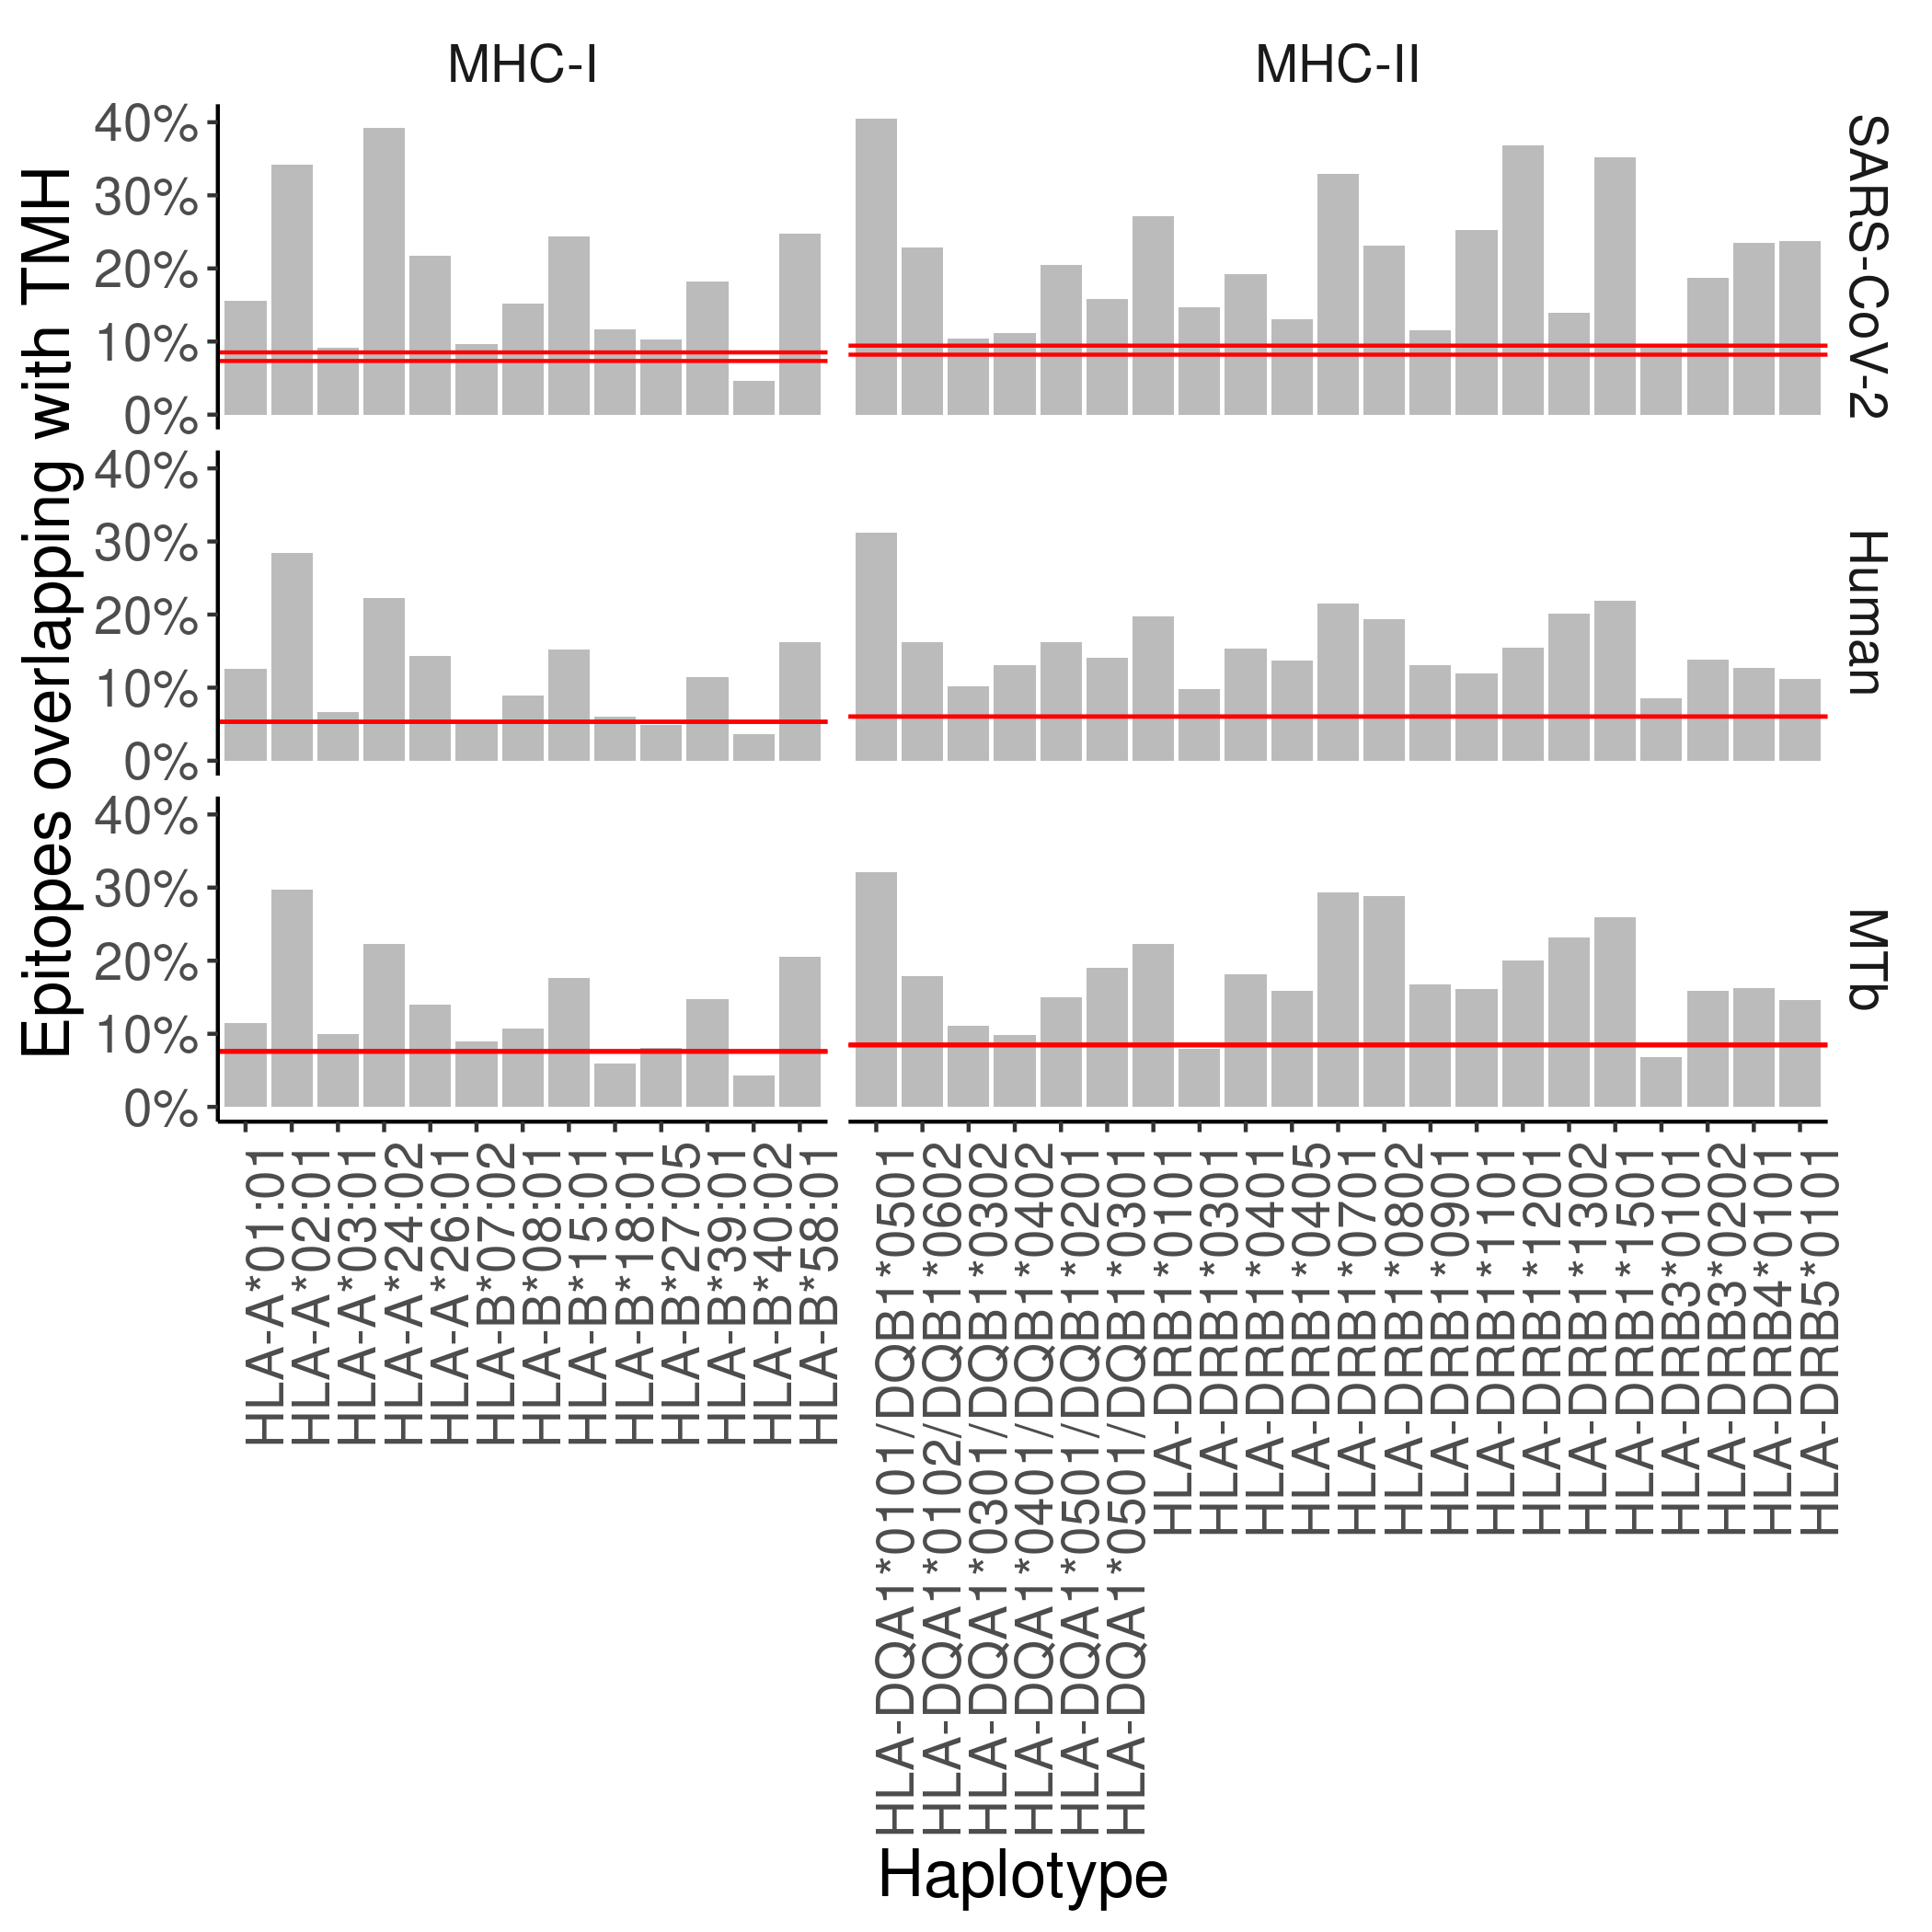
\includegraphics[width=0.95\textwidth]{bbbq_1_smart_results/fig_f_tmh_2_panel}
  \caption{
    TMH-derived peptides are predicted to be over-presented in general,
    which is for MHC-I (left column) and MHC-II (right column),
    as well as for the proteomes of SARS-CoV-2 (top row), human (middle 
    row) and \emph{M. tuberculosis} (bottom row).
    The bars show the percentage of epitopes predicted to be 
    overlapping with TMHs.
    The red lines indicate the percentage as expected by chance.
    See supplementary tables \ref{tab:tmh_binders_mhc1} and \ref{tab:tmh_binders_mhc2}
    for the exact TMH and  epitope counts.
    \richel{Add panel with hydrophobicity}
  }
  \label{fig:bbbq_1_smart_results}
\end{figure}

%%%%%%%%%%%%%%%%%%%%%%%%%%%%%%%%%%%%%%%%%%%%%%%%%%%%%%%%%%%%%%%%%%%%%%%%%%%%%%
\subsection{TMH-derived peptides are predicted to be over-presented in MHC-II}
%%%%%%%%%%%%%%%%%%%%%%%%%%%%%%%%%%%%%%%%%%%%%%%%%%%%%%%%%%%%%%%%%%%%%%%%%%%%%%

We next wondered if the over-representation of TMH-derived peptides would also be present for MHC-II. 
Figure \ref{fig:bbbq_1_smart_results} shows the percentages of MHC-II epitopes predicted to be overlapping 
with TMHs for our human, viral and bacterial proteomes.
See supplementary table \ref{tab:tmh_binders_mhc2} 
for the TMH and epitope counts.
We predict that TMH-derived peptides are also over-presented in most MHC-II haplotypes, and this over-presentation seems even more pronounced than for MHC-I. 
\richel{
  Showing how general our finding is (as it is explained by hydrophobicity)
  is important. See \url{https://github.com/richelbilderbeek/bbbq_article/issues/192}
}
Similar to our previous results with MHC-I, we predicted that the extent to which TMH-derived
epitopes are presented by each MHC-II haplotype is similar for the human, bacterial and viral proteome.


Plotting the normalized values of presented TMH-derived epitopes (where
$1.0$ denotes that the percentage of presented TMH-derived epitopes
matches the values as expected by chance) in \ref{fig:rel_presentation}
shows that MHC-II has a higher relative over-presentation of TMH-derived
epitopes, when compared to MHC-I.
The MHC-I molecule presents epitopes of shorter length than MHC-II.
We expect this to be of no influence in the presentation level
of TMH-derived epitopes, for each of the three proteomes.
We verified this, by normalizing the percentage of TMH-derived epitopes found
to the percentage of TMH-derived epitopes expected, 
where a value of $1.0$ denotes that the percentage of TMH-derived epitopes found
matches the percentage as expected by chance.
\richel{explain only the results found. Elaborate. Draw a conclusion}
Additionally, we investigated if MHC-I and MHC-II are equally prone
to present TMH-derived epitopes. 
\richel{Add exact method}
See \ref{fig:rel_presentation} and \ref{fig:rel_presentation_per_haplotype}.

%%%%%%%%%%%%%%%%%%%%%%%%%%%%%%%%%%%%%%%%%%%%%%%%%%%%%%%%%%%%%%%%%%%%%%%%%%%%%%
\subsection{TMH-derived peptides are predicted to be presented in vivo}
%%%%%%%%%%%%%%%%%%%%%%%%%%%%%%%%%%%%%%%%%%%%%%%%%%%%%%%%%%%%%%%%%%%%%%%%%%%%%%

\begin{figure}[!htbp]
  \centering
  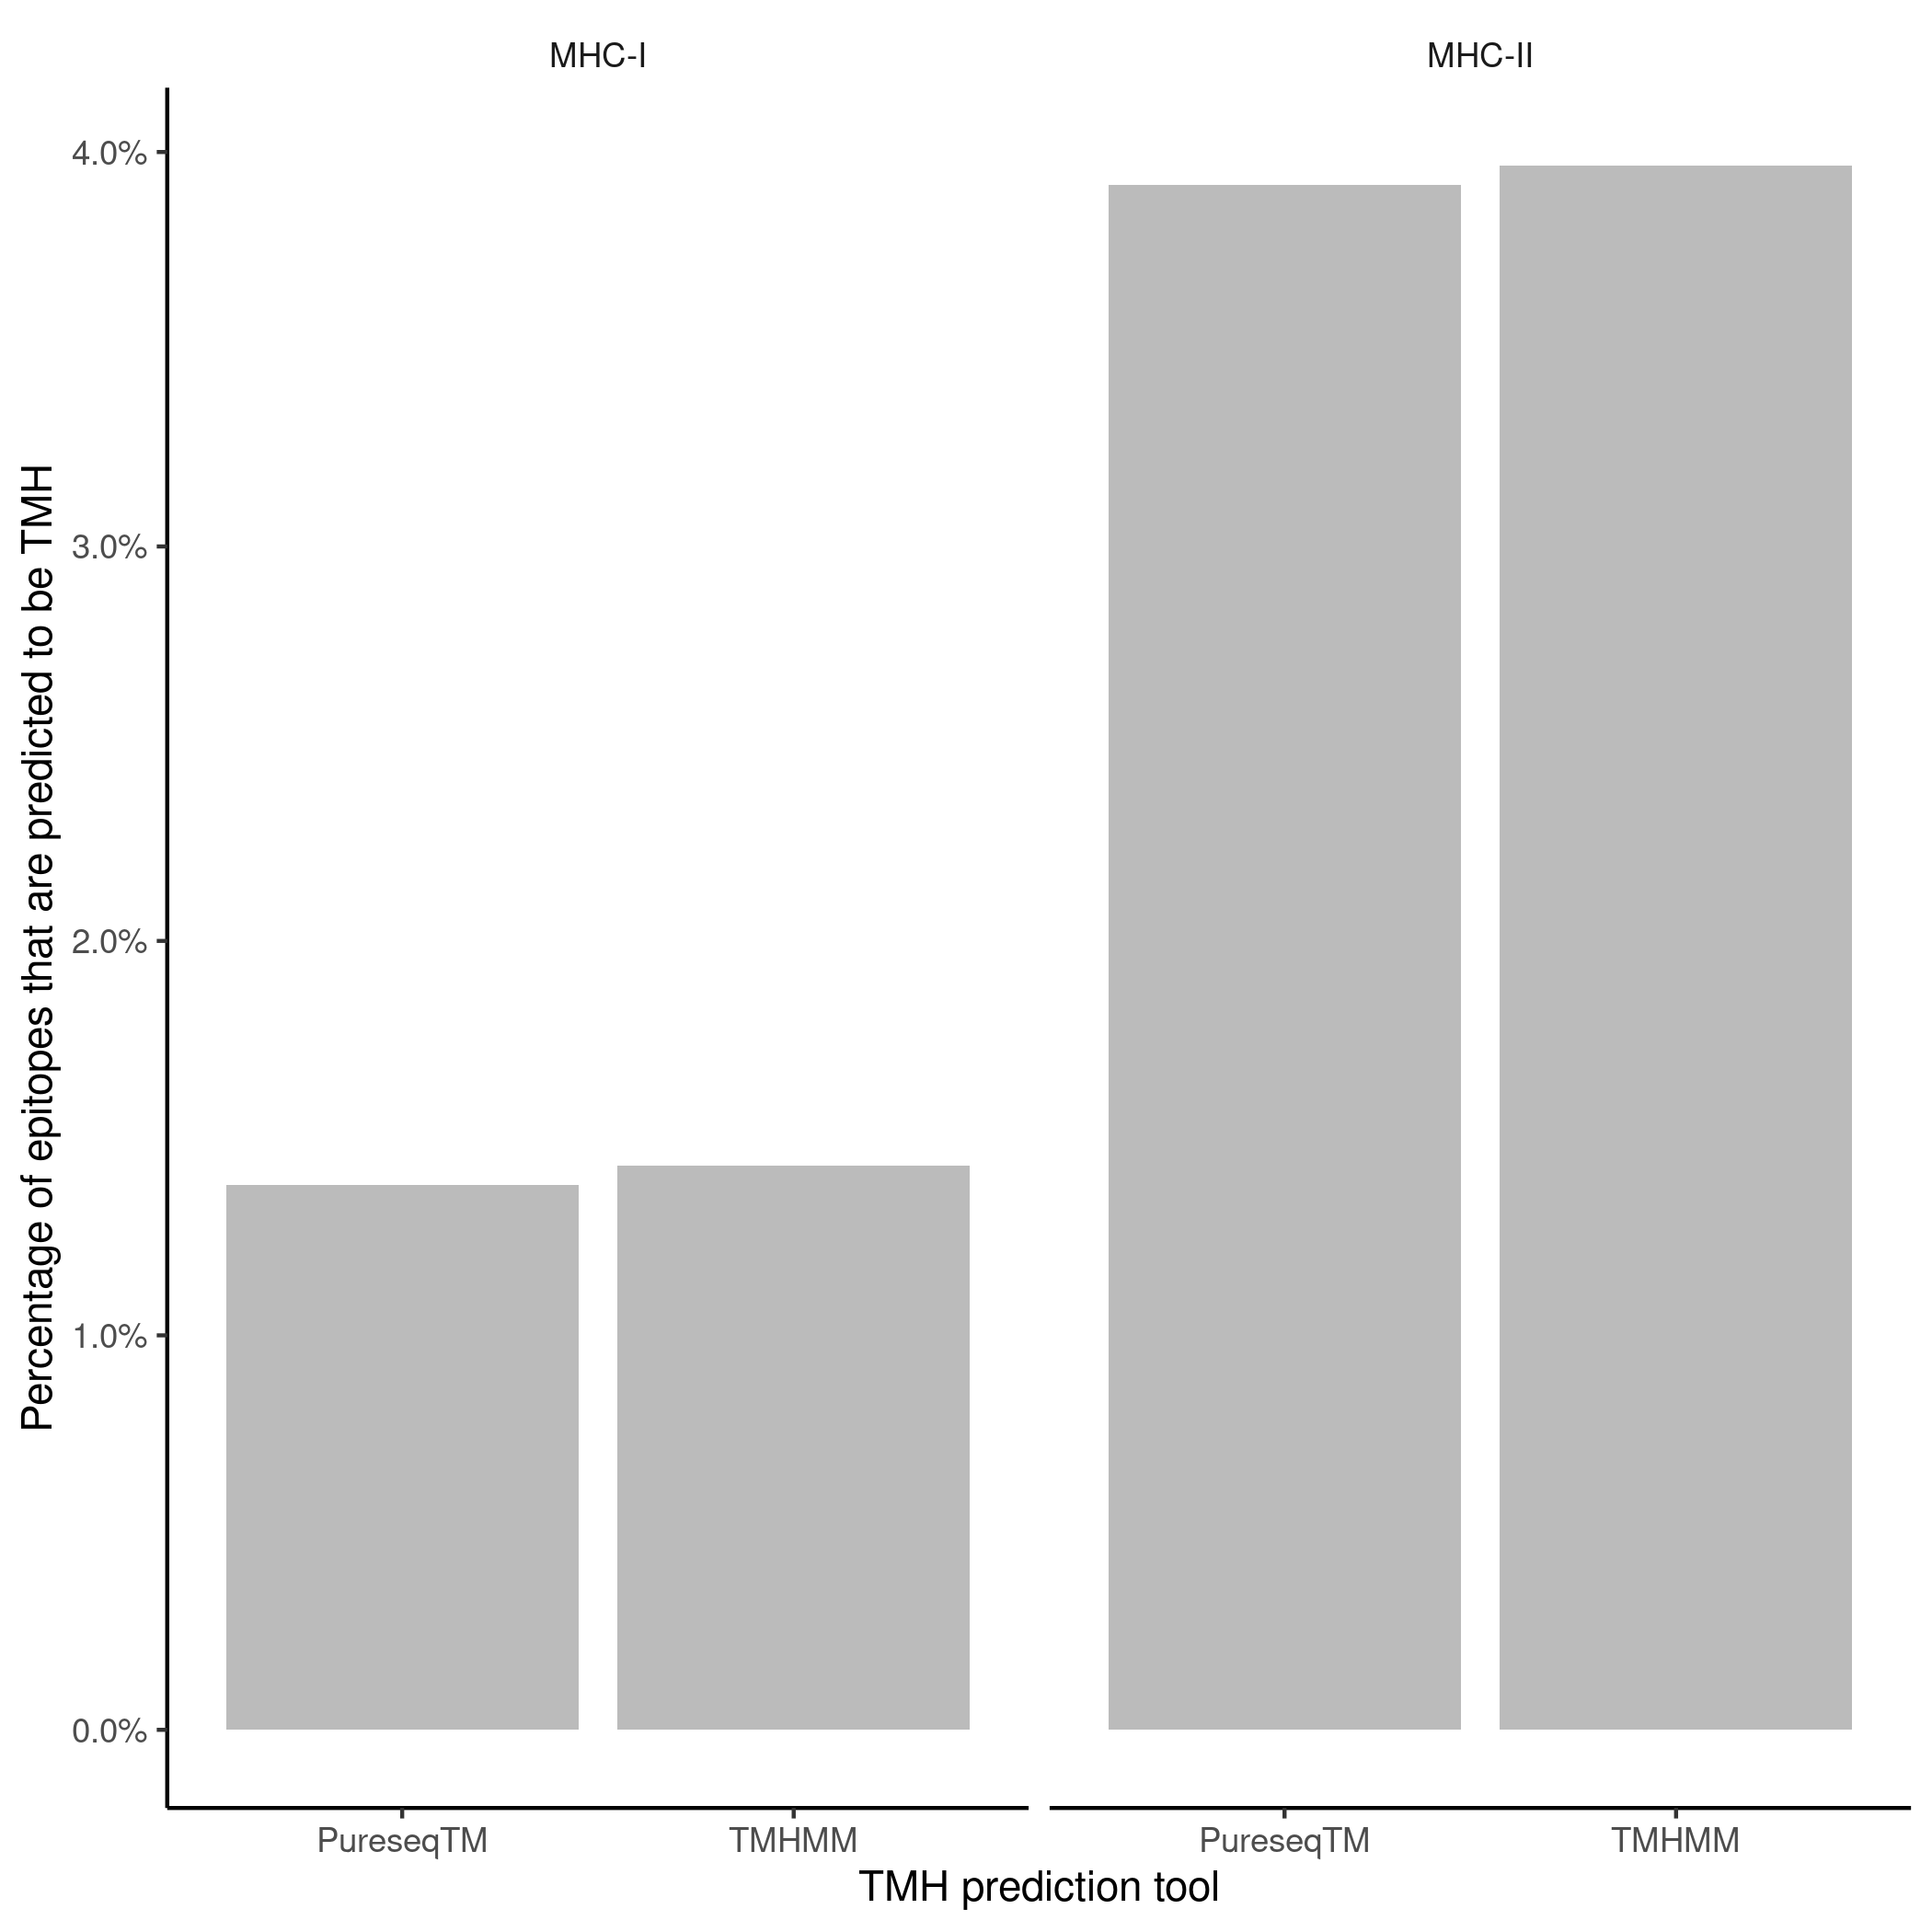
\includegraphics[width=0.5\textwidth]{bbbq_article_issue_157/results.png}
  \caption{
    TMH-derived epitopes are presented in vivo,
    for both MHC-I and MHC-II, for two topology prediction
    programs.
    See table \ref{tab:elution} for the exact values.
  }
  \label{fig:elution}
\end{figure}

To obtain experimental confirmation that peptides stemming from TMHs are presented in MHC-I and MHC-II,
peptide elution studies were reanalyzed.
Figure \ref{fig:elution} shows the percentages of epitopes derived 
from TMHs
found in the MHC-I (\cite{schellens2015comprehensive}) and MHC-II elution 
studies  (\cite{bergseng2015different}),
for the two topology prediction tools TMHMM (\cite{krogh2001predicting}) and PureseqTM (\cite{wang2019efficient}). 
Regardless of the prediction tool, 
at least 100 epitopes were predicted to be derived from a TMH for each condition. 
From these findings, it is robustly predicted that
epitopes derived from TMHs are presented in both MHC-I and MHC-II.

%%%%%%%%%%%%%%%%%%%%%%%%%%%%%%%%%%%%%%%%%%%%%%%%%%%%%%%%%%%%%%%%%%%%%%%%%%%%%%%%
\subsection{Human TMHs are evolutionarily conserved}
%%%%%%%%%%%%%%%%%%%%%%%%%%%%%%%%%%%%%%%%%%%%%%%%%%%%%%%%%%%%%%%%%%%%%%%%%%%%%%%%

\begin{figure}
  \centering
  \begin{subfigure}[t]{0.45\textwidth}
    \centering
    \caption{}
    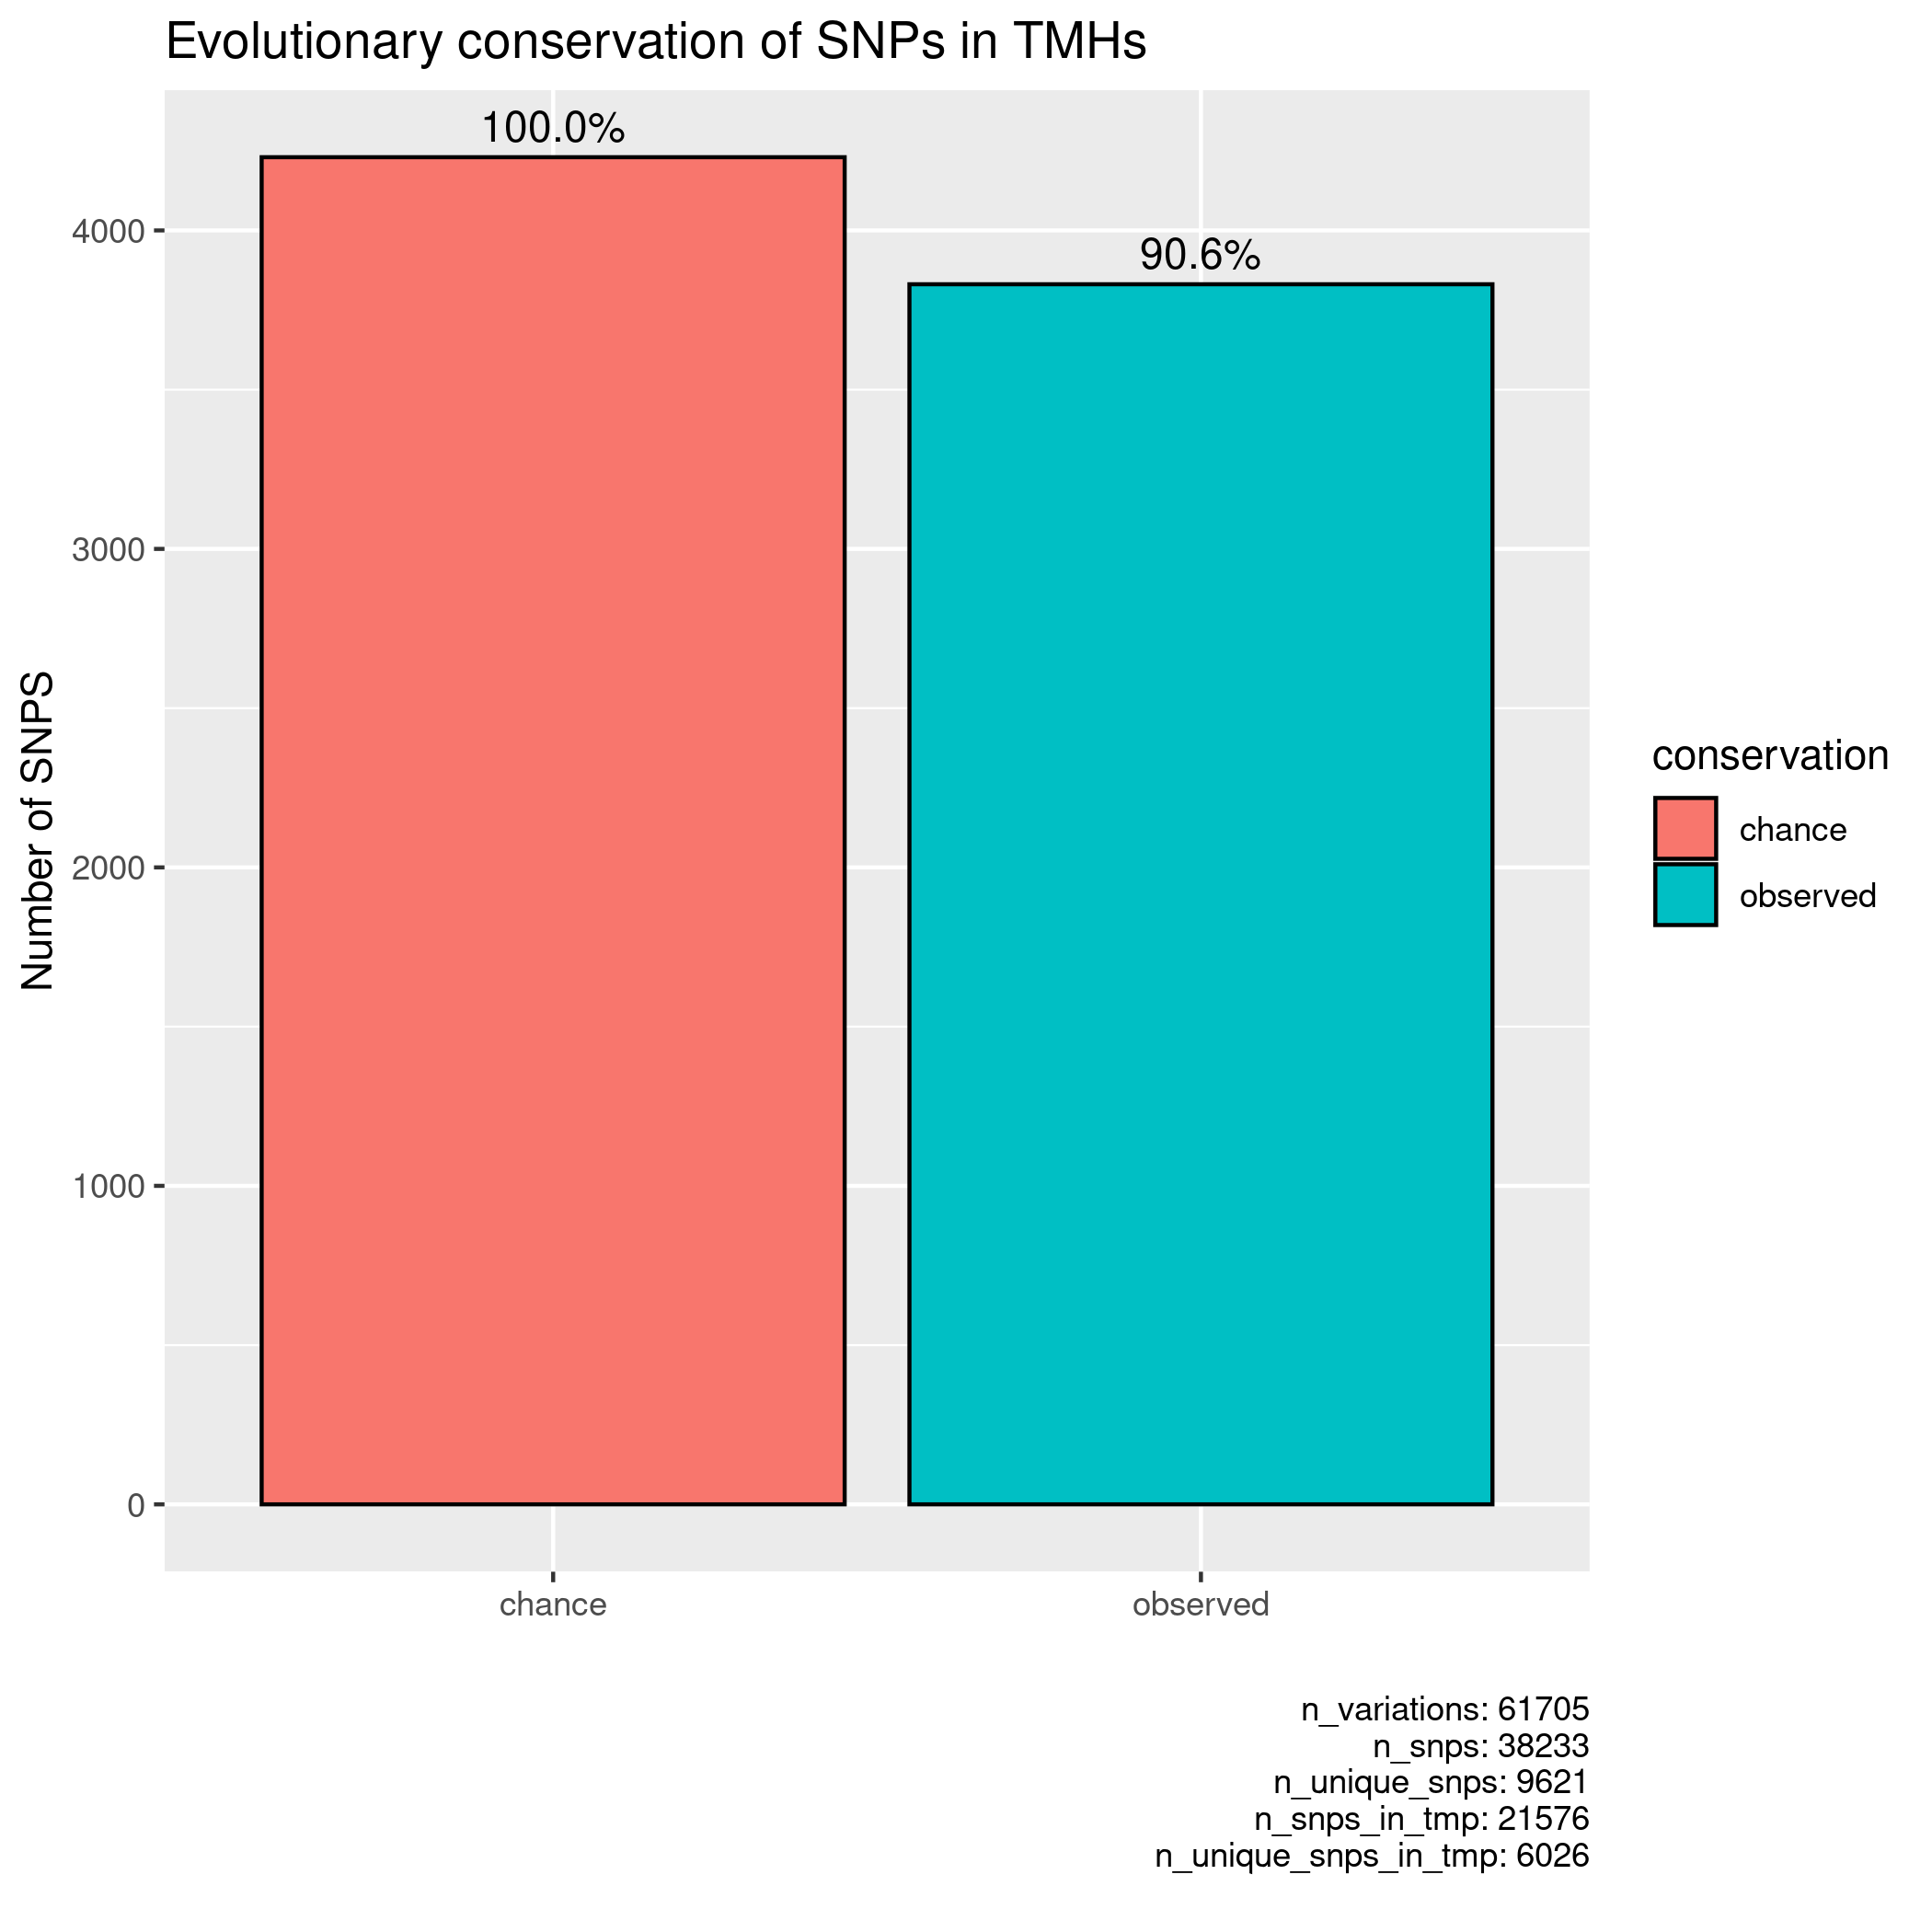
\includegraphics[width=\linewidth]{ncbi_peregrine_results/fig_conservation.png}
    \label{fig:conservation}
  \end{subfigure}
  \hfill
  \begin{subfigure}[t]{0.45\textwidth}
    \centering
    \caption{}
    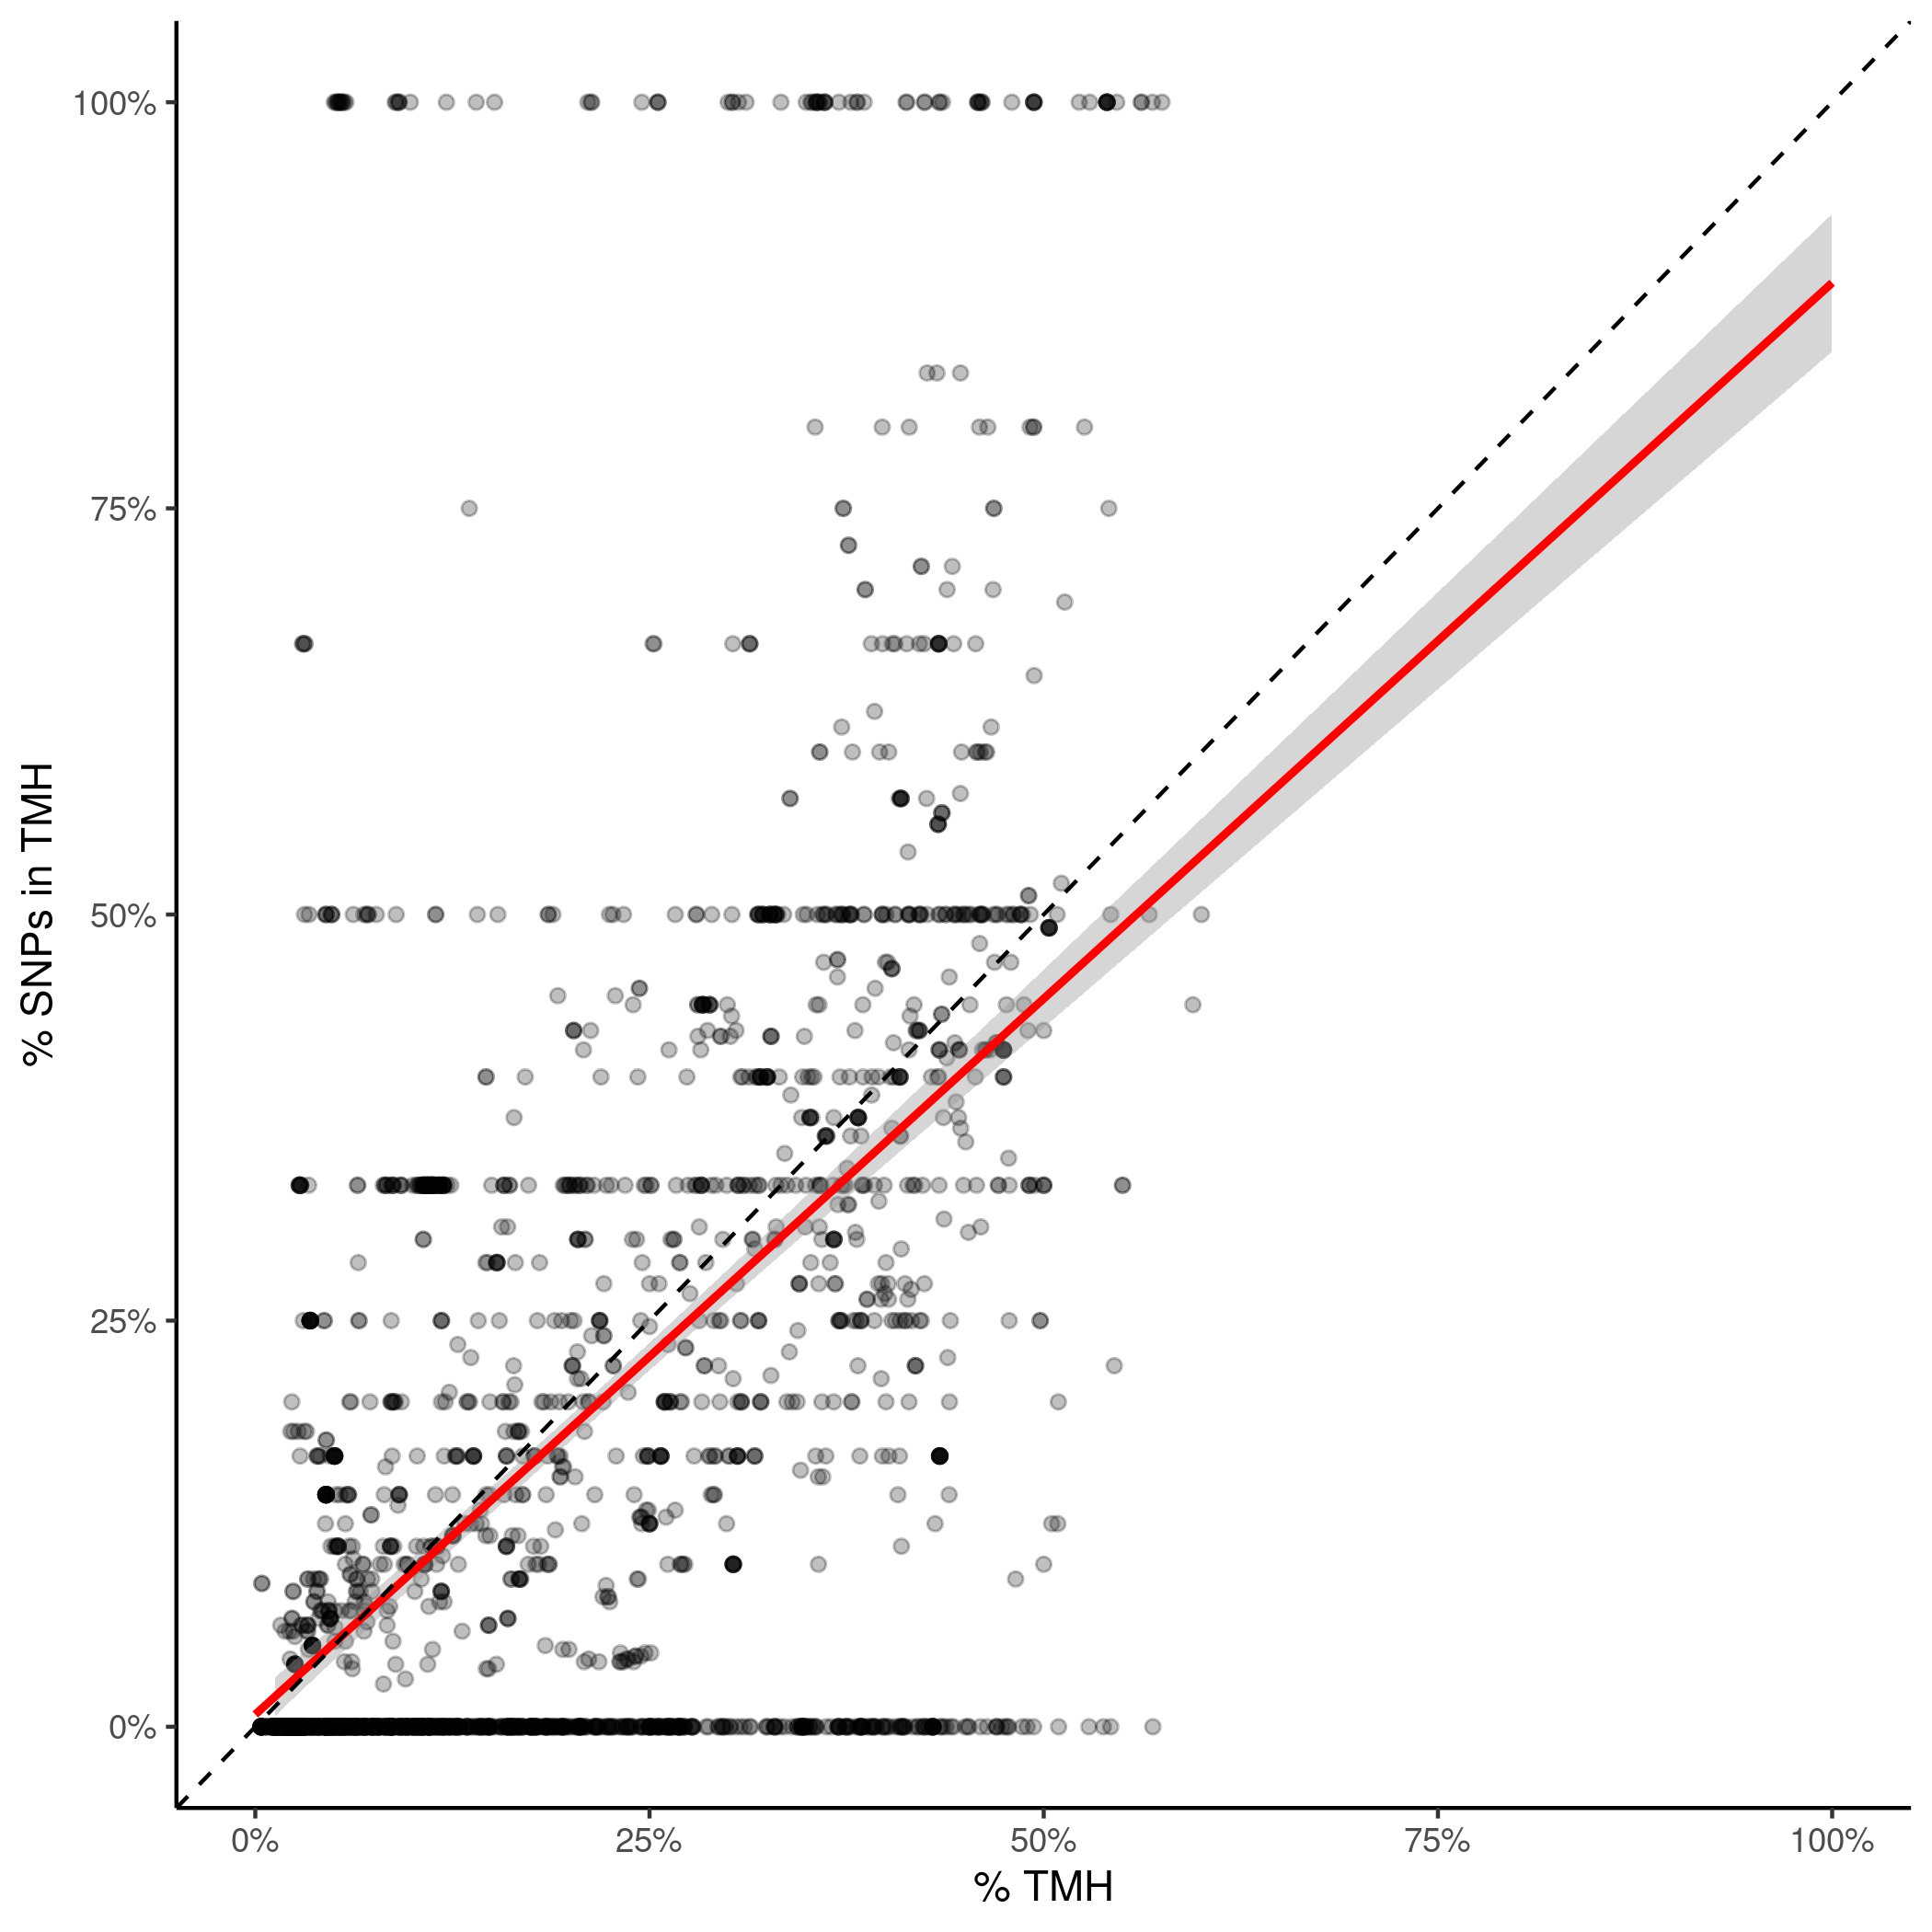
\includegraphics[width=\linewidth]{ncbi_peregrine_results/fig_f_snps_found_and_expected.png}
    \label{fig:f_snps_found_and_expected}
  \end{subfigure}
  
   \vfill

  \begin{subfigure}[t]{0.45\textwidth}
    \centering
    \caption{}
    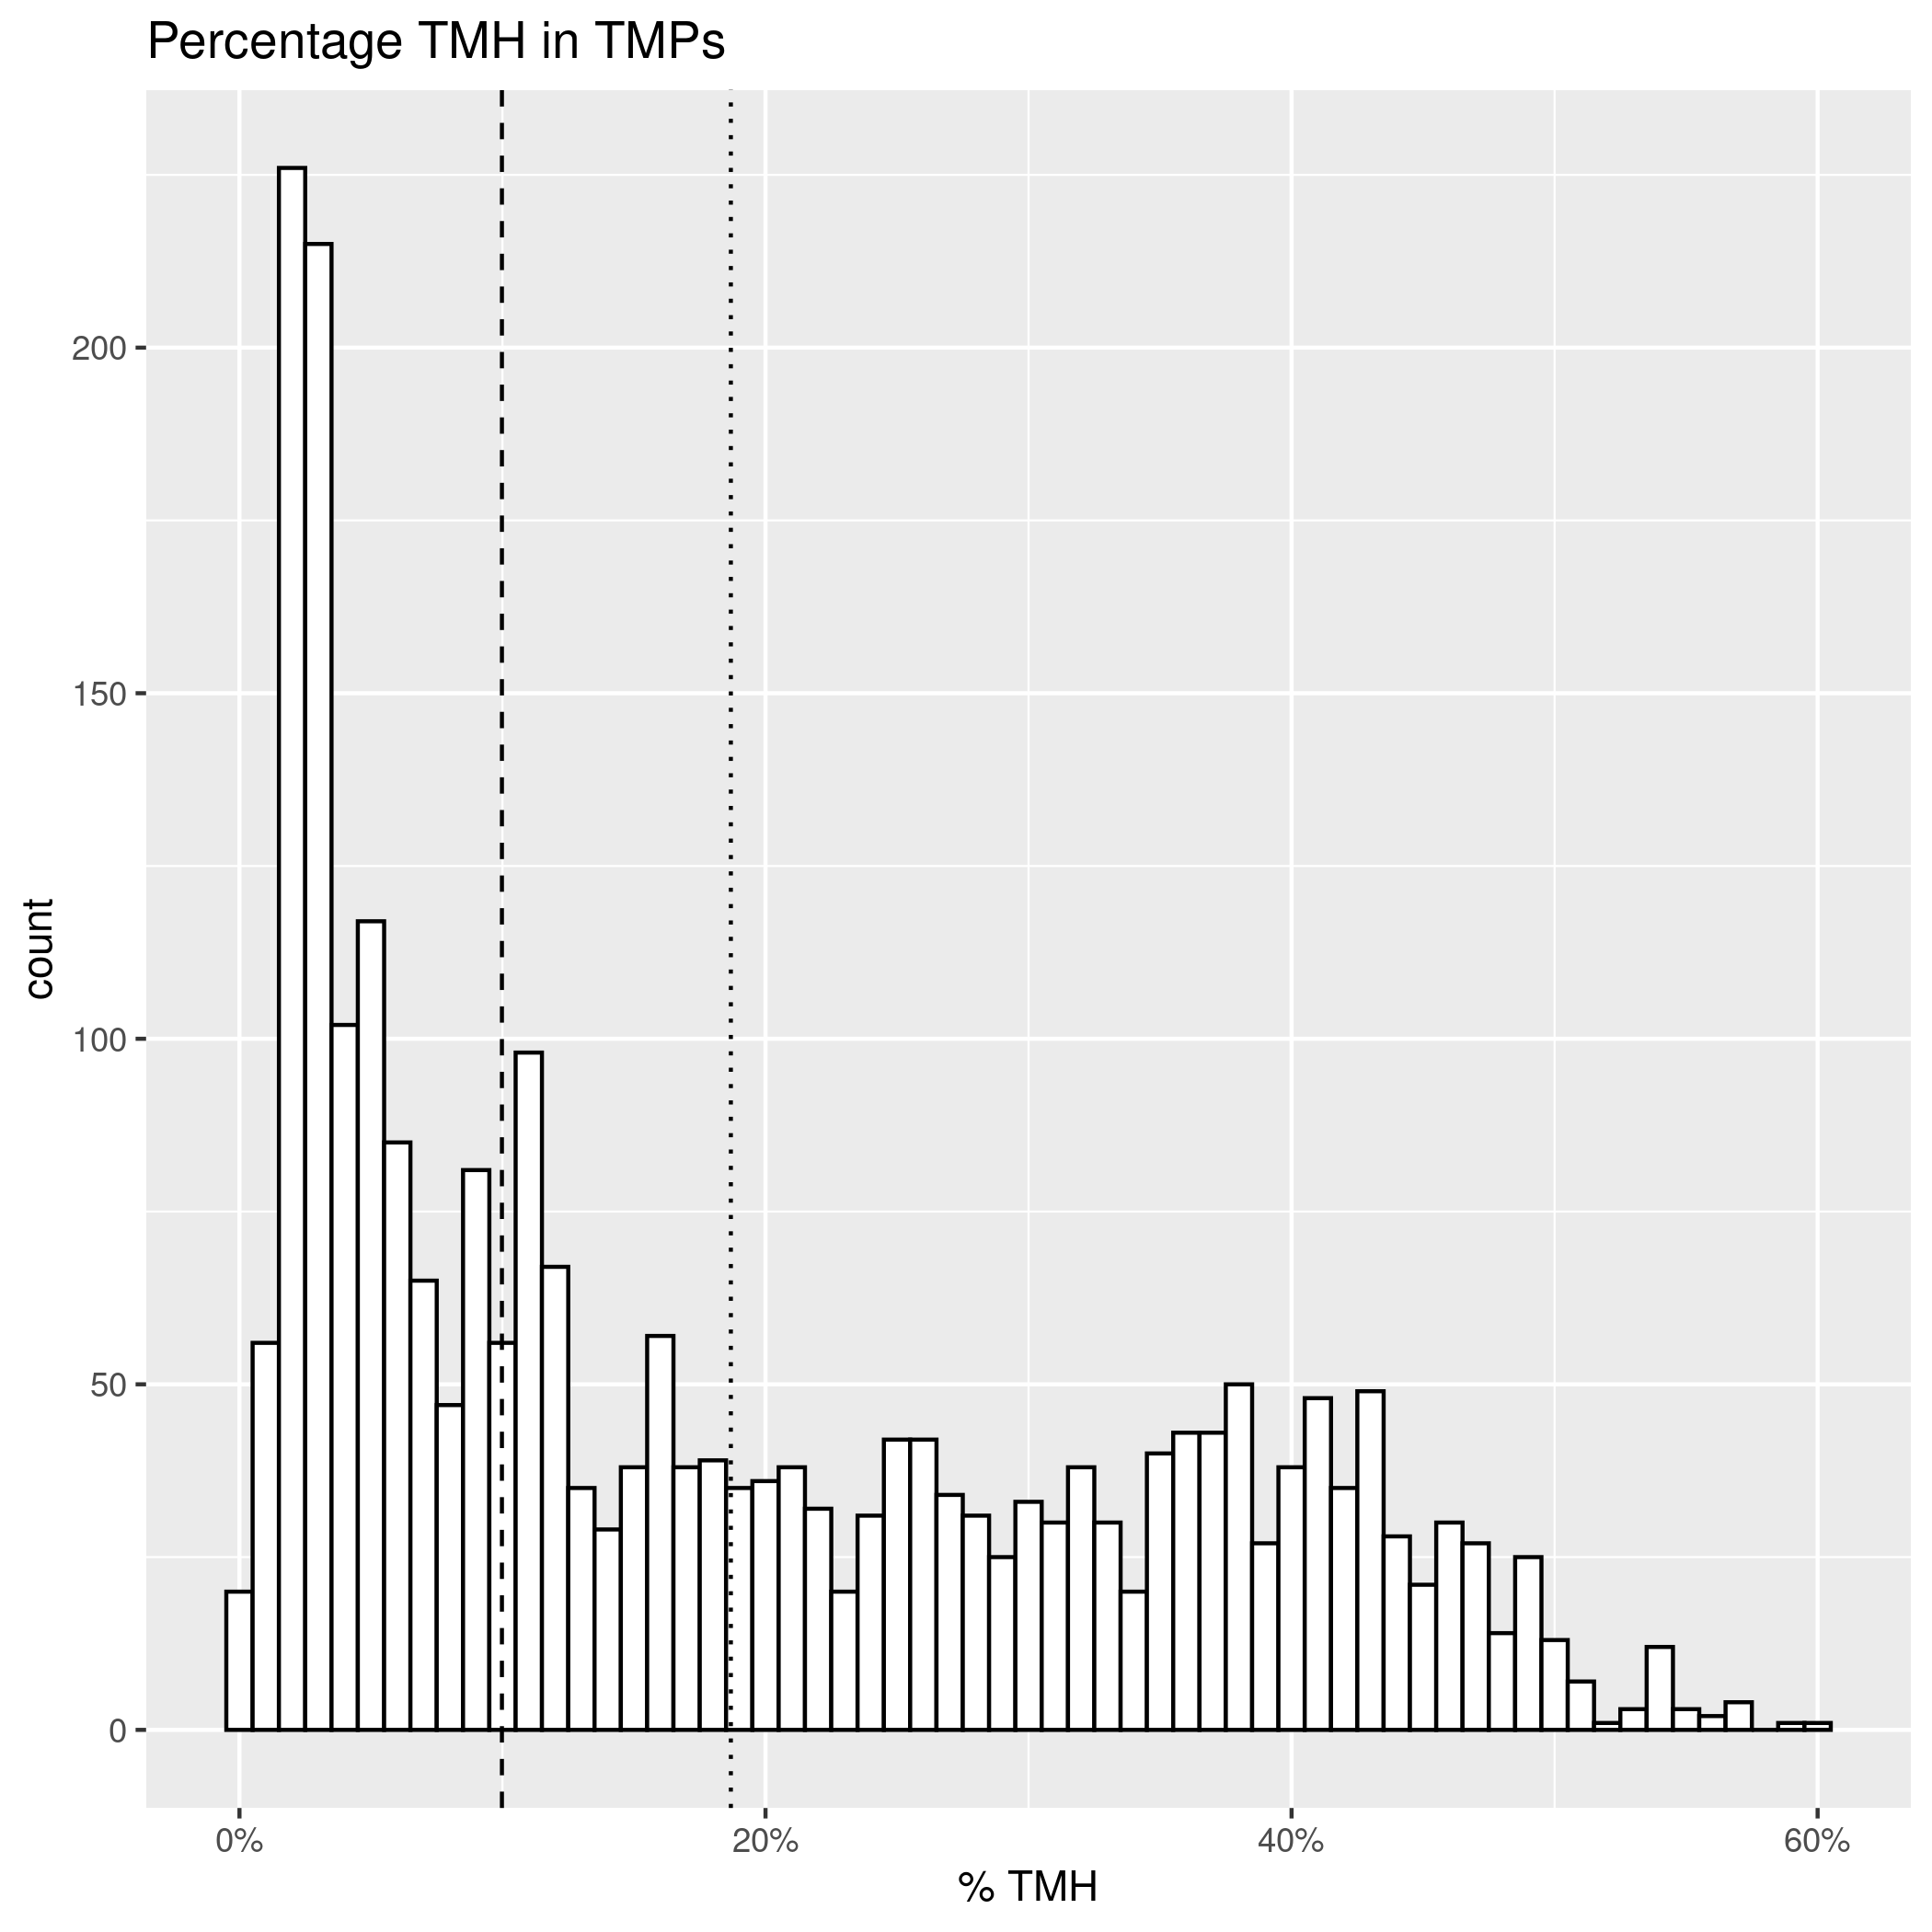
\includegraphics[width=\linewidth]{ncbi_peregrine_results/fig_f_tmh_ncbi.png}
    \label{fig:f_tmh_ncbi}
  \end{subfigure}  


  \caption{
    \textbf{(A)} 
    The number of SNPs in TMHs as expected by chance (left bar) 
    and found in the dbSNP database (right bar).
    Percentages are added to show the relative conservation
    of SNPs in TMHs found.
    \textbf{(B)}
    Percentage of SNPs found in TMHs.
    Each point shows the predicted percentage of
    TMH (x-axis) and the observed occurrence of SNPs being located
    within a TMH (y-axis) for a protein.
    The dashed diagonal line shows the line of equality (i.e.
    equal conservation of TMHs and soluble protein regions).
    The blue line is a linear trend line that includes only the
    transmembrane proteins.
    \textbf{(C)}
    Distribution of the percentages of TMH of TMPs.
  }
\end{figure}

\begin{figure}
  \centering
  \begin{subfigure}[t]{0.45\textwidth}
    \centering
    \caption{}
    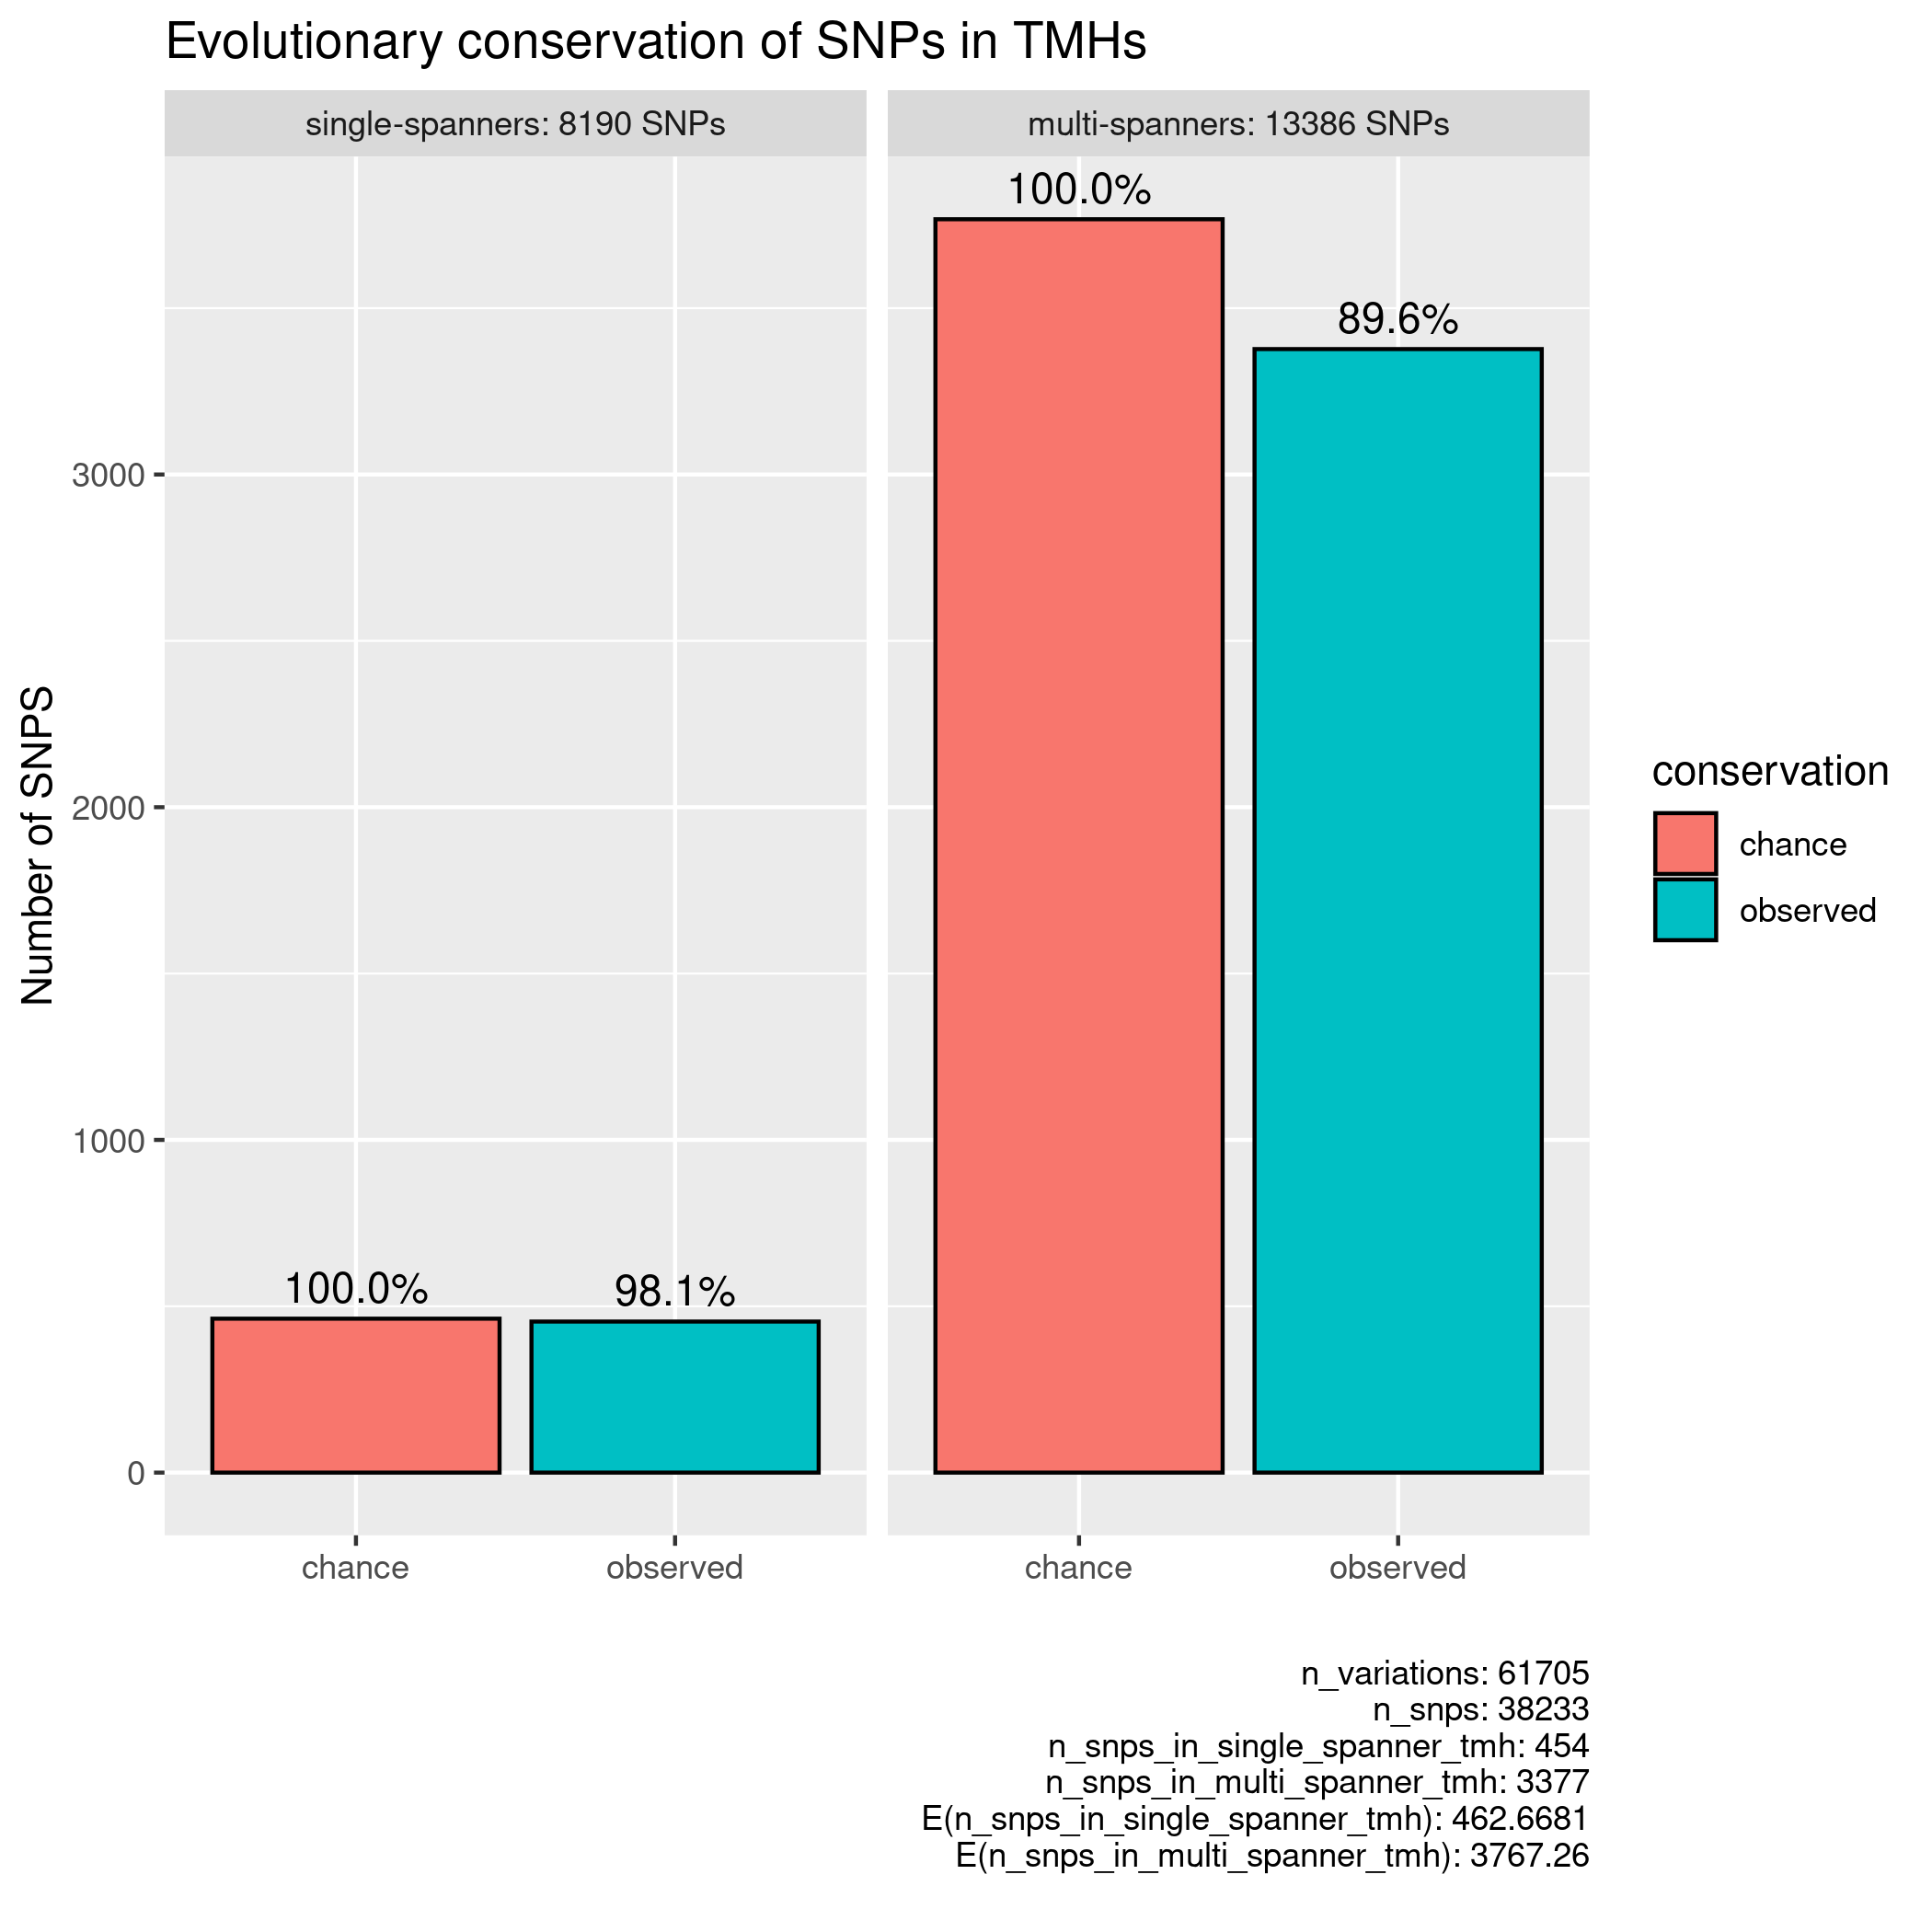
\includegraphics[width=\linewidth]{ncbi_peregrine_results/fig_conservation_per_spanner.png}
    \label{fig:conservation_per_spanner}
  \end{subfigure}
  \hfill
  \begin{subfigure}[t]{0.45\textwidth}
    \centering
    \caption{}
    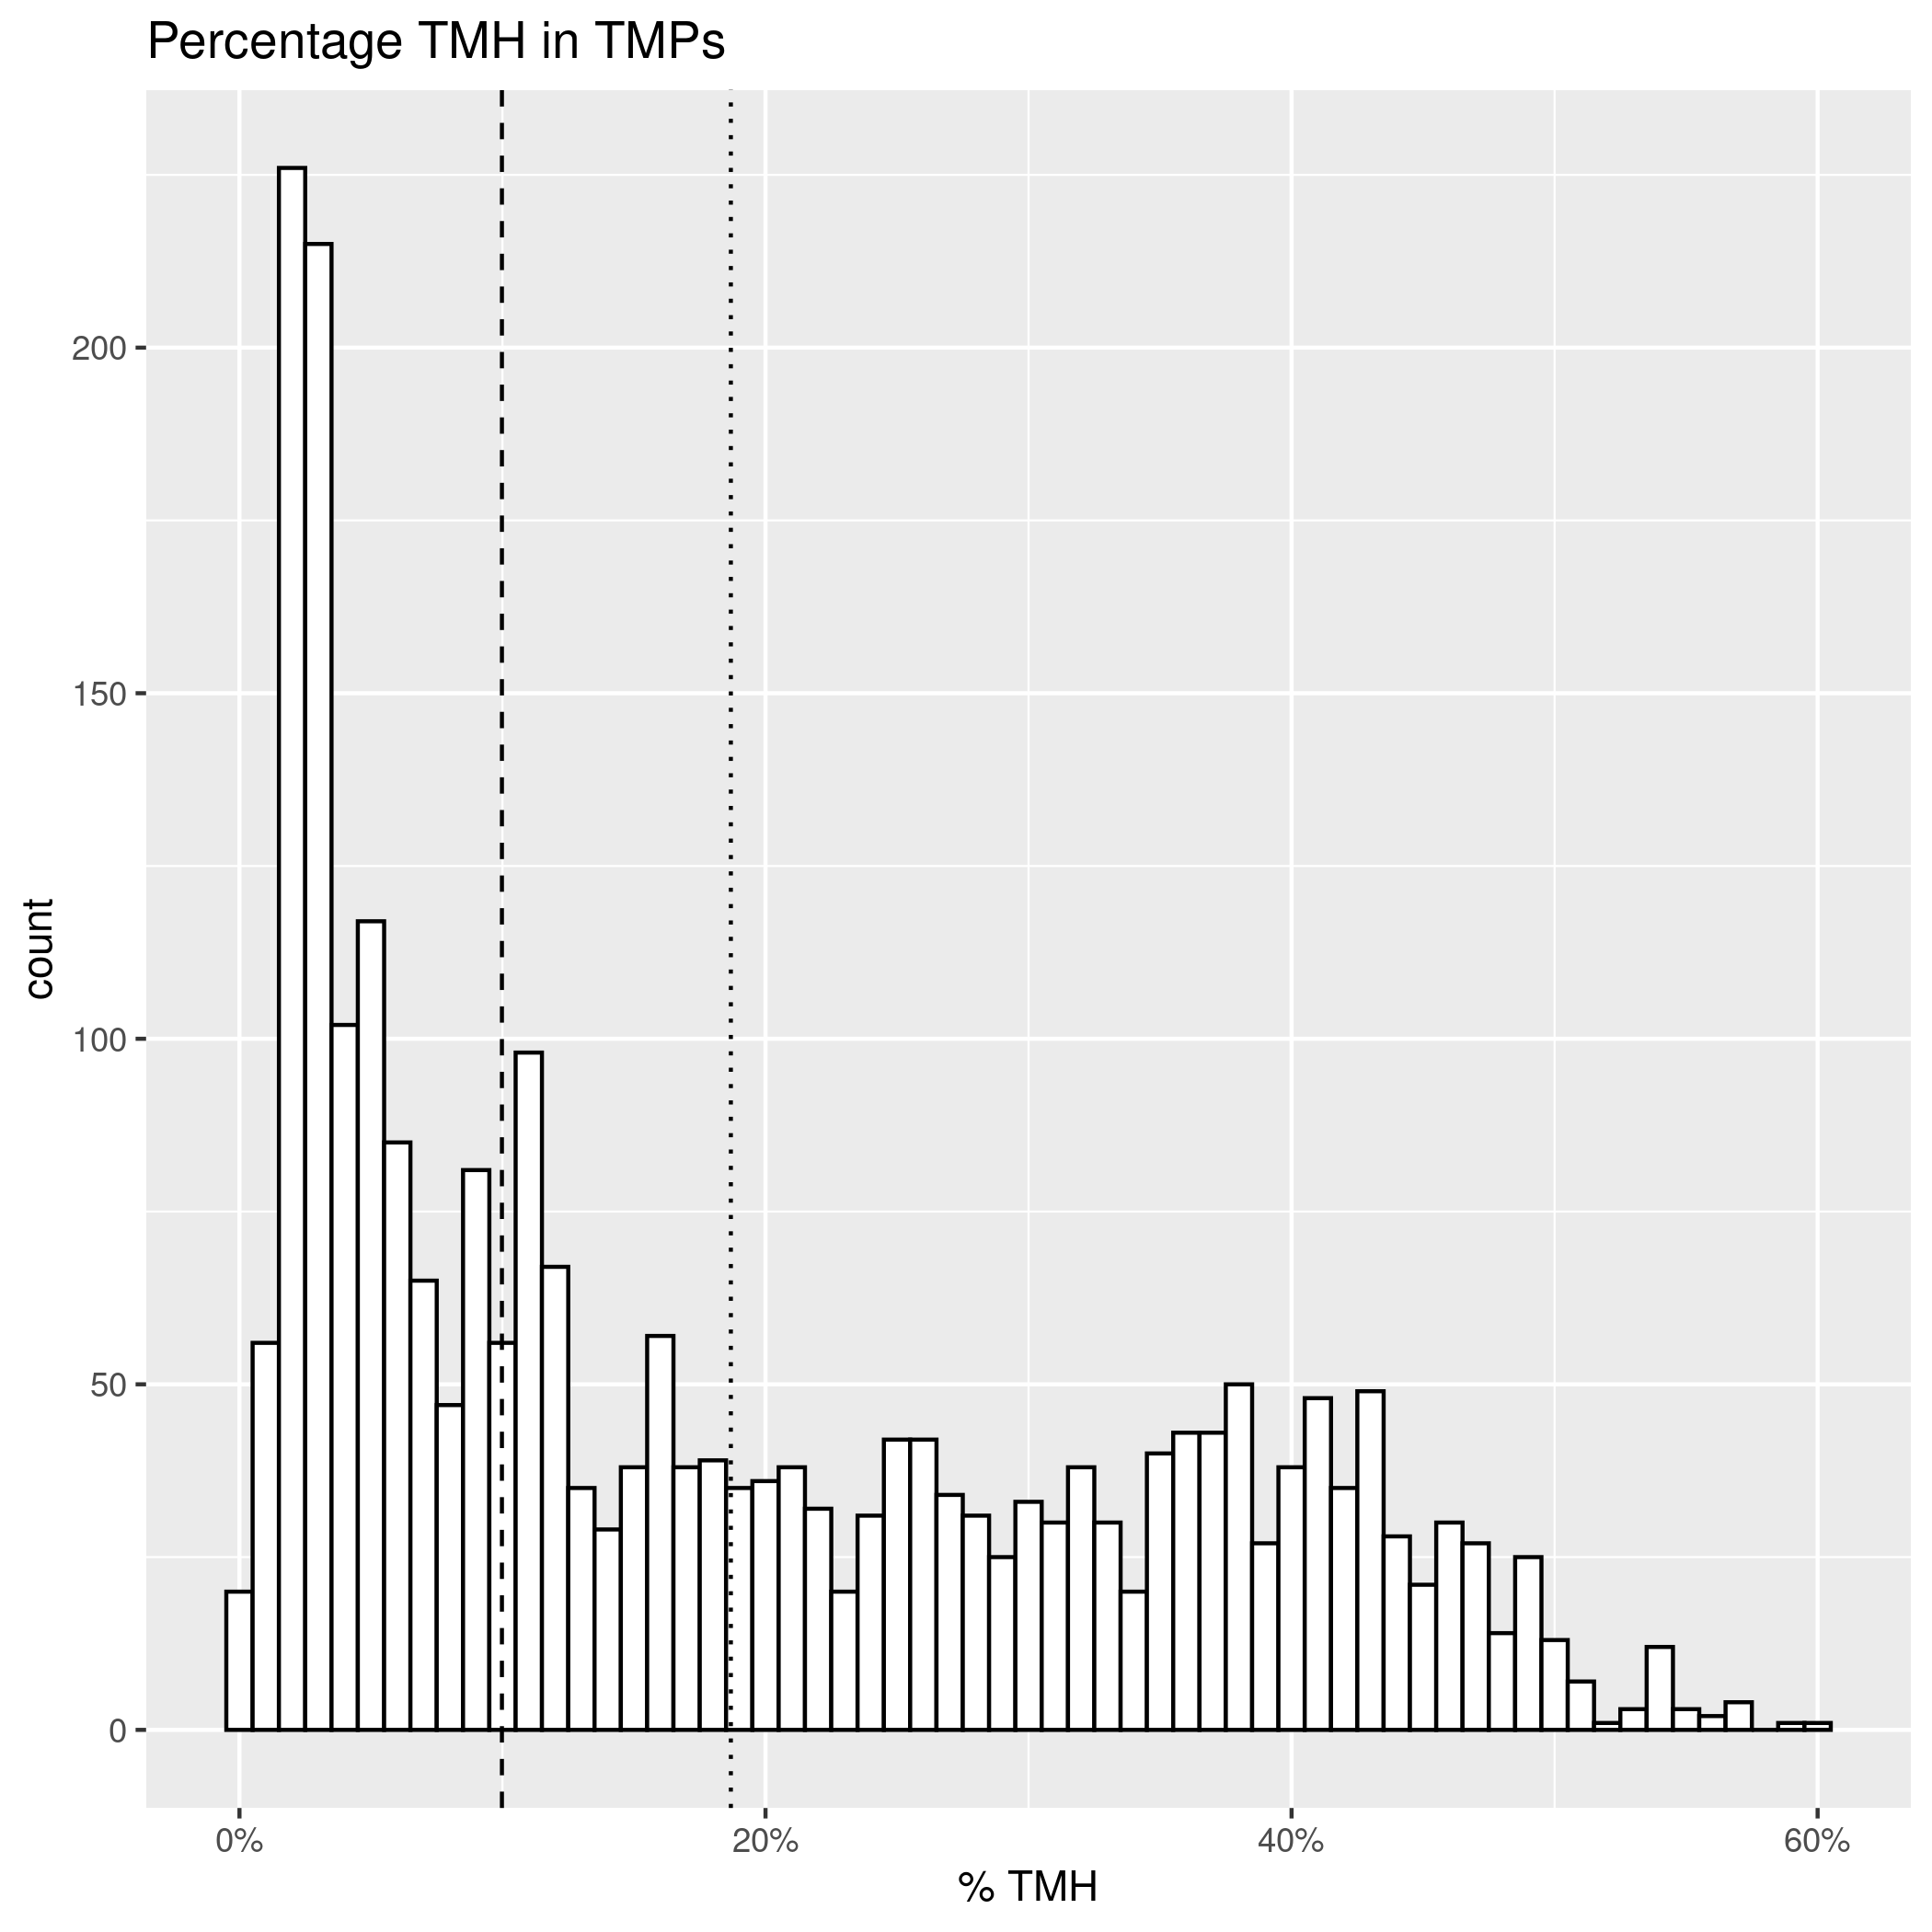
\includegraphics[width=\linewidth]{ncbi_peregrine_results/fig_f_tmh_ncbi.png}
    \label{fig:f_tmh_ncbi_per_spanner}
  \end{subfigure}  

  \vfill
  
  \begin{subfigure}[t]{\textwidth}
    \centering
    \caption{}
    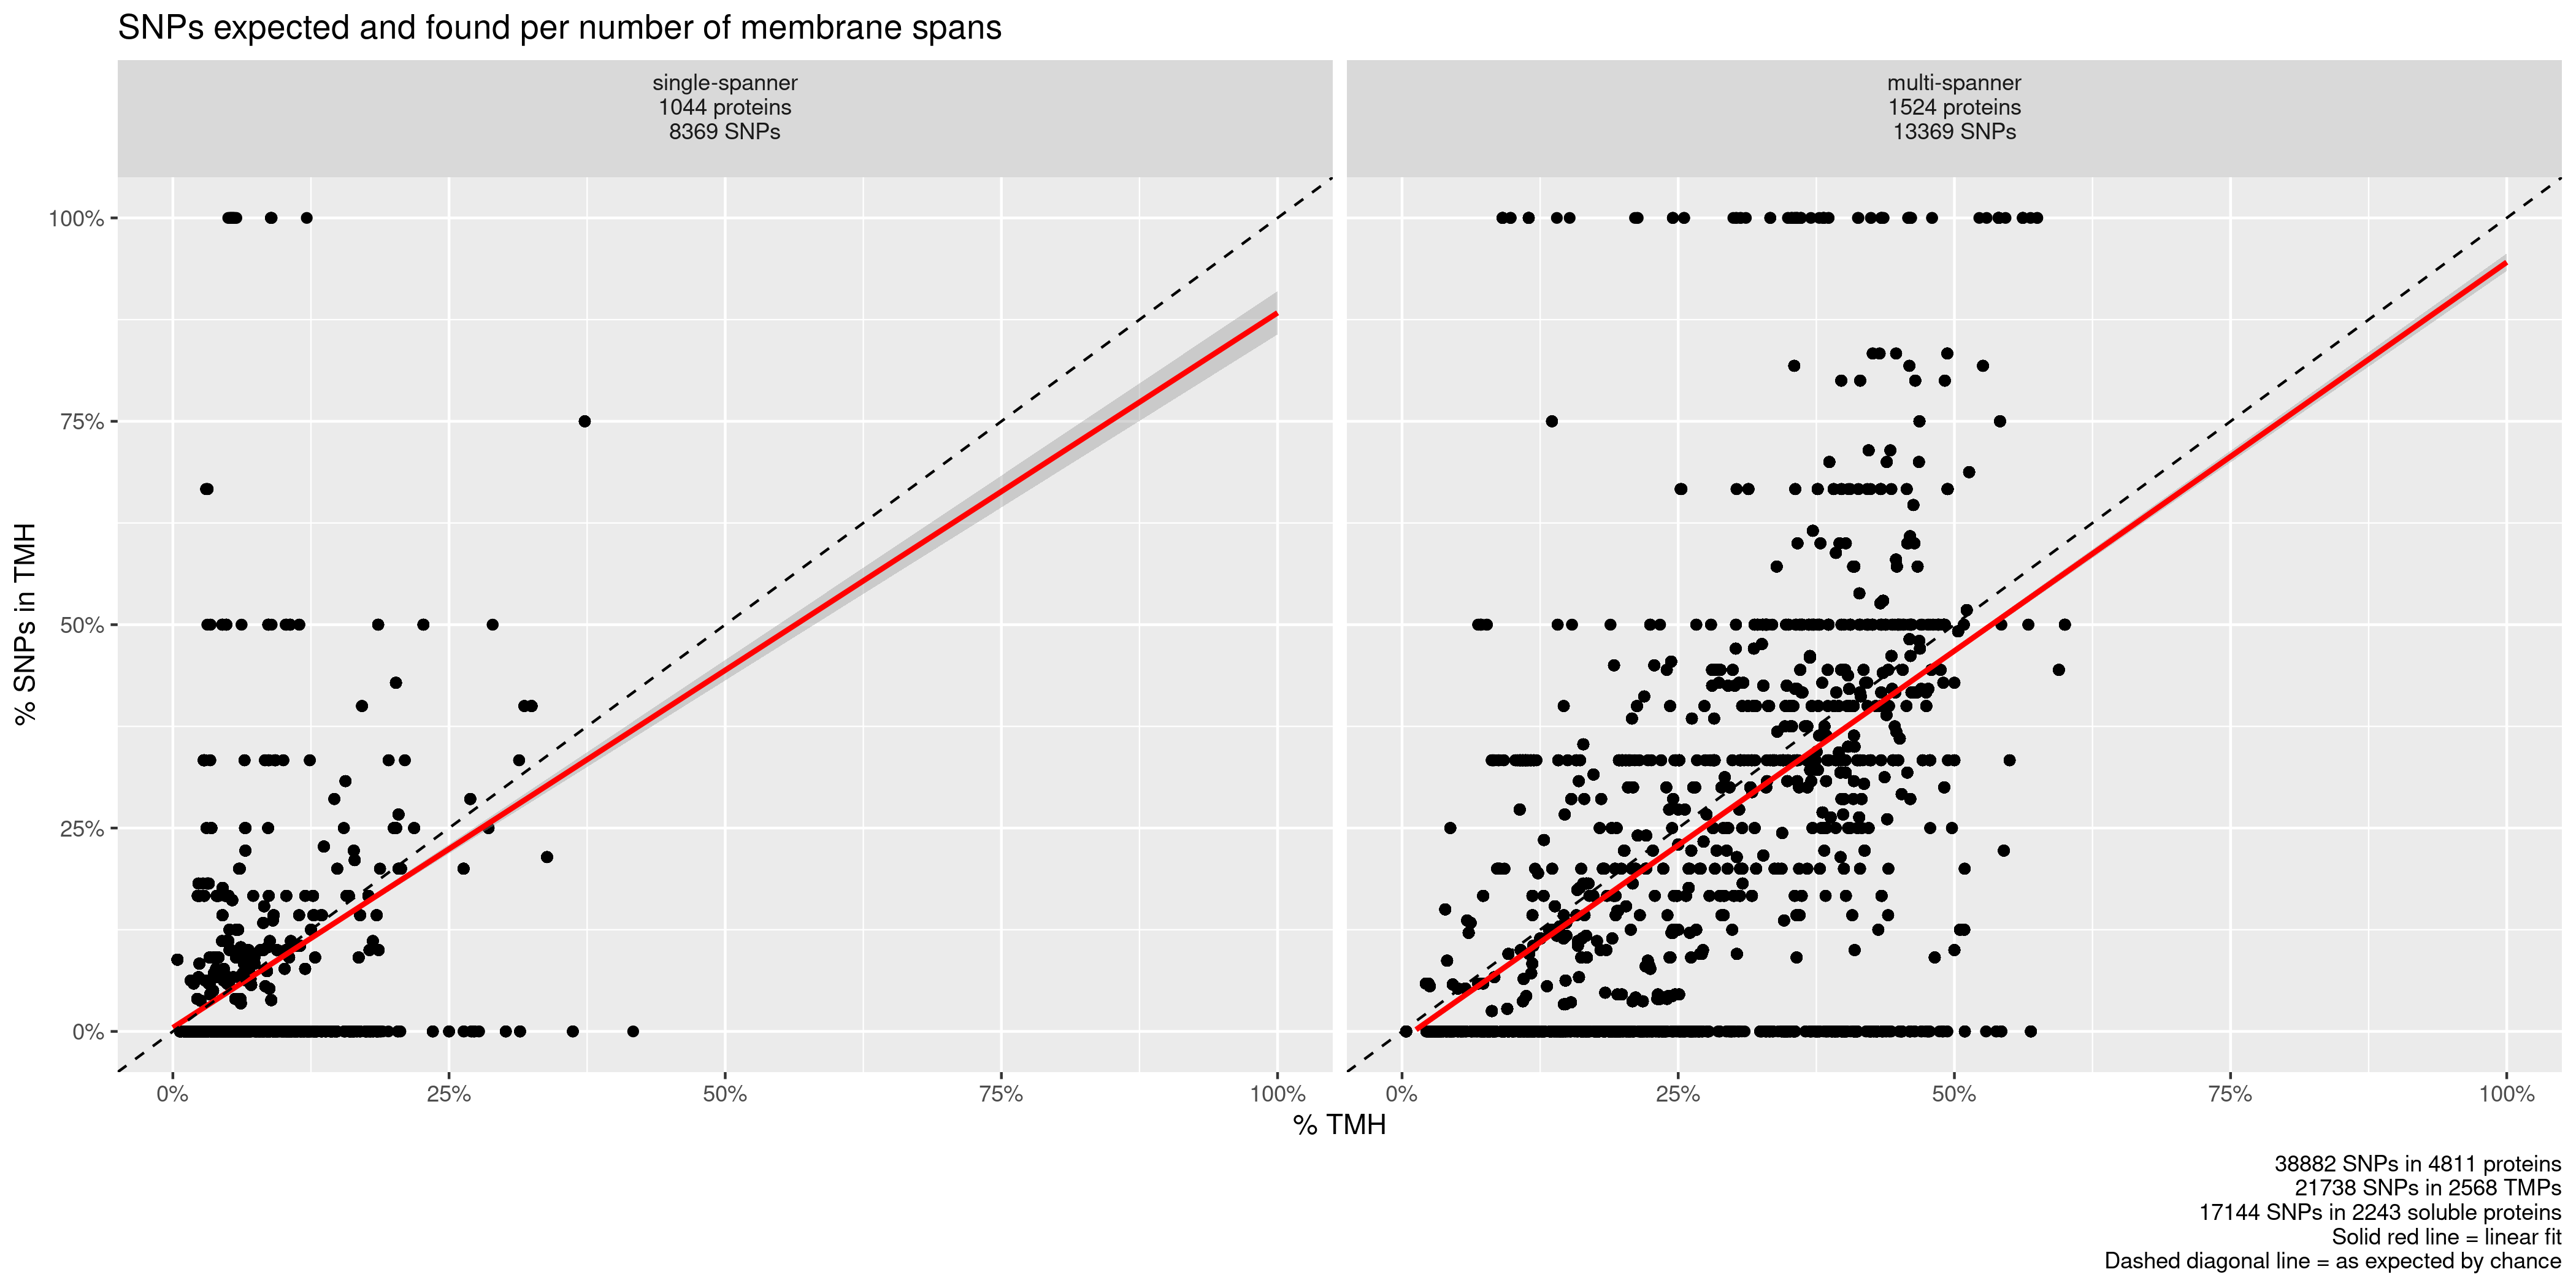
\includegraphics[width=\linewidth]{ncbi_peregrine_results/fig_f_snps_found_and_expected_per_spanner.png}
    \label{fig:f_snps_found_and_expected_per_spanner}
  \end{subfigure}
  \caption{
      \textbf{(A)} 
      The number of SNPs in TMHs as expected by chance (red bars) 
      and found in the dbSNP database (right bars), 
      after splitting the data into single- and multi-spanners.
      Percentages are added to show the relative conservation
      of SNPs in TMHs found.
      \textbf{(B)} 
      \richel{THIS IS A PLACEHOLDER}
      Distribution of the proportion of amino acids residing
      in the plasma membrane.
      \textbf{(C)} 
      Percentage of SNPs found in TMPs predicted to have only a single
      (left) or multiple (right) TMHs.
      The dashed diagonal lines show the expected line of equality 
      (i.e., equal conservation of TMHs and solvent-exposed 
      protein regions).
  }
\end{figure}

We addressed the question whether there is an evolutionary advantage in presenting TMHs. We determined the conservation of TMHs by comparing the occurrences of SNPs located in TMHs or solvent-exposed protein regions for the genes coding for membrane proteins.
We obtained $>$1,000 gene names associated with the phrase 'membrane protein',
which are genes for both membrane-associated proteins (MAPs, no TMH) and 
transmembrane proteins (TMPs, at least one TMH).
These genes are linked to 4,780 protein isoforms, 
of which 2,553 are predicted to be TMPs and 
2,237 proteins are predicted to be MAPs.
We obtained 37,630 SNPs that resulted in an
amino acids substitution, of which 21,024 were located 
in predicted TMPs.
See tables \ref{tab:ncbi_counts_1} and \ref{tab:ncbi_counts_2} 
for the detailed numbers and distributions of SNPs.

Per protein, we calculated two percentages: 
(1) the percentage of the total protein predicted to be TMHs, 
and (2) the percentage of SNPs located within these predicted TMHs.
Each percentage pair was plotted in figure \ref{fig:f_snps_found_and_expected}.
Most our TMPs had less than half their residues located in the 
plasma membrane.
The proportion of SNPs found in TMHs varied from 
none (i.e. all SNPs were in
soluble regions) to all.
To determine if it is likelier to find SNPs within either TMHs or
soluble-facing domains, we performed a linear regression analysis,
and added a 95\% confidence interval on this regression.
This linear fit nearly goes through the origin and has a slope
below the line of equality,
which shows that less SNPs are found in TMHs than expected by chance.

We determined the probability to find the observed amount
of SNPs in TMHs by chance, i.e. when assuming SNPs occur 
just as likely in soluble domains as in TMHs.
We used a binomial Poisson distribution, 
where the number of trails ($n$) equals the number of SNPs, 
which is 21,208. 
The probability of success for the $i$th TMP ($p\_i$), 
is the percentage of residues within a TMH per TMP. 
These probabilities are shown as a histogram 
in figure \ref{fig:f_tmh_ncbi}). 
The expected number of SNPs expected to be found in 
TMHs by chance equals $\sum{p} \approx 4,141$.
As we observed 3,903 SNPs in TMHs, 
we calculated the probability of having that amount or less successes.
We used the type I error cut-off value of $\alpha = 2.5\%$.
The chance to find, within TMHs, this amount or less SNPs 
equals $6.8208 \cdot 10^{-11}$.
We determined the relevance of this finding, by
calculating how much less SNPs are found in TMHs,
when compared to soluble regions, which is the
ratio between the number of SNPs found in TMHs
versus the number of SNPs as expected by chance.
In effect, per 1000 SNPs found in soluble protein domains, 
one finds 918 SNPs in TMHs,
as depicted in figure \ref{fig:conservation}. 

We split this analysis based on the number of TMHs
of each TMP. 
We hypothesized that single-membrane spanners (i.e., proteins
with a single predicted TMH) are less conserved than multi-membrane spanners (with $>$1 TMH),
because multi-membrane spanners
might have protein-protein interactions between their TMHs, 
for example to accommodate active sites, and 
thus might have additional structural constraints.
From the split data, we did the same analysis:
figure \ref{fig:f_snps_found_and_expected_per_spanner} 
shows, the percentage a protein resides in the membrane versus the
percentage of SNPs found in those TMH regions, per spanner.
In both cases, a linear regression shows that less
SNPs are found in TMHs, than expected by chance.

Also per spanner, we determined the probability to find the 
observed amount of SNPs in TMHs by chance.
For single-spanners, we found 452 SNPs in TMH, where
$\approx462$ were expected by chance. 
The chance to observe this or a lower number by chance is 
$0.319$. As this chance was higher than our $\alpha = 0.025$
and we considered this no significant effect.
For the single-spanners, we found 3,351 SNPs in TMH, where
$\approx3678$ were expected by chance. 
The chance to observe this or a lower number by chance is 
$8.315841 \cdot 10^{-12}$, 
which means we attribute the lower number of SNPs found
to an effect, instead of luck. 

Also, per spanner type, 
we determined the relevance of this finding, by
calculating how much less SNPs are found in TMHs,
when compared to soluble regions,
as depicted in figure \ref{fig:conservation_per_spanner}.
In effect, per 1000 SNPs found in soluble protein domains, 
one finds 978 SNPs in TMHs 
in single spanners (although this is not significant)
and 911 SNPs in TMHs in multi-spanners.

%%%%%%%%%%%%%%%%%%%%%%%%%%%%%%%%%%%%%%%%%%%%%%%%%%%%%%%%%%%%%%%%%%%%%%%%%%%
\section{Discussion}
%%%%%%%%%%%%%%%%%%%%%%%%%%%%%%%%%%%%%%%%%%%%%%%%%%%%%%%%%%%%%%%%%%%%%%%%%%%

% \paragraph{General}

Epitope prediction is 
important to understand the immune system and for the design of vaccines. In this study, we provide evidence that epitopes
derived from TMHs are a major but overlooked source of MHC epitopes. Both our bioinformatics predictions and reanalysis of peptide elution studies show that TMH-derived epitopes are 
presented more often than expected by chance, regardless of the organism. Moreover, our SNP analysis shows  
that TMHs are evolutionary more conserved than solvent-exposed protein regions.

%%%%%%%%%%%%%%%%%%%%%%%%%%%%%%%%%%%%%%%%%%%%%%%%%%%%%%%%%%%%%%%%%%%%%%%%%%%
\subsection{TMH-derived epitopes are predicted to be presented in vivo}
%%%%%%%%%%%%%%%%%%%%%%%%%%%%%%%%%%%%%%%%%%%%%%%%%%%%%%%%%%%%%%%%%%%%%%%%%%%

% \paragraph{Over-presentation in vivo in MHC-I and MHC-II is robust
We show that 1.4\% of epitopes that are naturally presented on MHC-I 
can be mapped to stem from a TMH. We also find that MHC-II presents epitopes derived from TMHs in vivo, as we find that 3.9-4.0\% of sequenced epitopes
can be uniquely traced onto a human reference 
proteome (also shown in table \ref{tab:elution}).

% \paragraph{TMH presentation in vivo}

Although elution studies and in silico predictions both suggest that TMH-derived epitopes are presented in MHC-I and MHC-II, the molecular mechanisms of how integral membrane proteins are processed for MHC presentation are largely unknown (\cite{bianchi2017}). Most prominently, the fundamental principles of how TMHs are extracted from the  hydrophobic lipid environment into the aqueous vacuolar lumen, and their prior or subsequent proteolytic processing are unresolved.
\geert{
  beetje kort. Suggesties? Experimental approaches? Hoeft niet super
  origineel, bijvoorbeeld suggereren dat lipases een rol kunnen spelen. Frans kan vast helpen met mooie zin
}

% \paragraph{False positives}

An important caveat of the elution studies is that we assume that 
the found epitopes are derived from their completely 
translated predecessor proteins.
However, there are multiple cellular processes 
that may result in peptide fragments that did not originate 
from the mature proteins.
One such process is the production of defective ribosomal 
products (DRiPs) (\cite{yewdell1996defective}),
in which the ribosome terminates its translation prematurely,
intrudes a point mutation, 
or cause a frame shift, at low frequencies (\cite{yewdell2011drips}).
Another process that results in peptide fragments absent in the
proteome is peptide fusion, 
in which peptides form covalent bonds with other peptides,
as is for example found in mice (\cite{delong2016pathogenic}).
Due to these processes, we may incorrectly attribute an
epitope to a specific proteome locations, 
where in reality, it was created de novo.
This may lead to false positives, as we incorrectly deduce
epitopes to be derived from a TMH, instead of from one of
these processes. Both processes, however, are thought to
occur at low frequencies (\cite{yewdell2011drips,delong2016pathogenic}).

Another caveat is that the TMH prediction tools are imperfect.
This imperfection, however, appears to be of limited importance,
as our data show that two different topology prediction software algorithms give similar results.
Additionally, this 
prediction is robust, as it holds for two TMH prediction tools, 
as shown by table \ref{tab:elution}).

A final caveat in the elution studies is that there is methodological bias caused by mass spectronomy,
as hydrophobic fragments are detected less 
by mass spectronomy (\cite{bianchi2017}). This means that the number of TMH-derived epitopes
might be underestimated.

%%%%%%%%%%%%%%%%%%%%%%%%%%%%%%%%%%%%%%%%%%%%%%%%%%%%%%%%%%%%%%%%%%%%%%%%%%%
\subsection{TMH-derived epitopes are presented more often than expected by chance}
%%%%%%%%%%%%%%%%%%%%%%%%%%%%%%%%%%%%%%%%%%%%%%%%%%%%%%%%%%%%%%%%%%%%%%%%%%%

% \paragraph{Over-presentation in silico}

Not only do we predict that MHC-I and MHC-II TMH-derived epitopes 
are presented, we conclude that these are additionally
presented more often than expected by chance 
alone (figure \ref{fig:bbbq_1_smart_results}).
This in silico finding is a general pattern 
that persists in both MHC-I and MHC-II, 
for humans, bacteria and viruses. 

% \paragraph{MHC-II is expected to present TMHs}
The results from this study support our hypothesis 
that TMH-derived epitopes are over-presented
in MHC-II, similarly to we previously showed for MHC-I (\cite{bianchi2017}). 
The over-presentation of TMHs for most MHC-II haplotypes 
appears to follow a similar pattern as MHC-I haplotypes,
although MHC-II presents slightly more TMH-derived
epitopes (see Supplementary Materials, figure \ref{fig:rel_presentation}
for a direct comparison). 
Unlike MHC-I, the human proteome over-presents TMH-derived
epitopes for all MHC-II haplotypes that we have investigated.
Possible there are MHC-II haplotypes that present less TMH-derived
epitopes than expected by chance.
The haplotype \verb;HLA-DQA1*0101/DQB1*0501; had the highest
over-presentation of TMH-derived epitopes,
which we suggest is the haplotype of choice 
to investigate the intracellular mechanism of TMH-derived
antigen presentation.

Our study also suggests that T cells will largely recognize 
different protein regions than B cells. 
Presentation of antigens by MHC-II is important 
for the activation of naive B cells by helper T cells. 
For this activation, 
B cells first ingest antigen that is bound to their B cell receptor, 
and subsequently present peptides derived from this antigen in MHC-II 
to helper T cells. 
Following their activation by the T cells, 
B cells mature into plasma cells 
and release antibodies which recognize the same part of the antigen 
as the original B cell receptor. 
B cell receptors and antibodies will thus recognize solvent-exposed regions 
of antigens that are accessible for binding to the B cell receptor. 
However, the results from our study predict that most MHC-II haplotypes 
present relatively hydrophobic peptides, 
which are less likely to be solvent exposed. 
It is unknown why B and T cells seem to predominantly recognize 
different protein regions, but one possibility might be that 
this lowers the chance of B cell mediated autoimmune diseases, 
because auto-reactive B and T cells recognizing different part 
of the same antigen would need to be present for breakage of B cell tolerance. 

%%%%%%%%%%%%%%%%%%%%%%%%%%%%%%%%%%%%%%%%%%%%%%%%%%%%%%%%%%%%%%%%%%%%%%%%%%%
\subsection{Less SNPs in TMHs found, hinting at evolutionary conservation}
%%%%%%%%%%%%%%%%%%%%%%%%%%%%%%%%%%%%%%%%%%%%%%%%%%%%%%%%%%%%%%%%%%%%%%%%%%%

We find that mutations are more likely to occur
in soluble regions of proteins, than in TMHs.
When selecting SNPs at random, per 1000 SNPs found in a soluble domain, 
one finds on average 918 SNPs in TMHs.
This effect is more pronounced in multi spanners likely as these TMHs more often serve additional functions, besides spanning the lipid bilayer. 

% \paragraph{Selection undetectable in whole proteome}
 
In general, one would hope that evolutionary selection results in
an immune system that as most attentive for protein regions that are
essential for the survival, proliferation and/or virulence or pathogenic microbes, as these will be most conserved.
In SARS-CoV-2, for example, there is preliminary evidence that the strongest
selection pressure is upon residues that change its 
virulence (\cite{velazquez2020positive}).
These regions, however, only account for a small part of a pathogen's proteome.
Additionally, these essential parts might differ widely between different pathogenic proteins.
Because of this scarcity and variance in targets, 
one can imagine that it will be mostly unfeasible to provide innate immune responses against such essential protein regions, 
as hinted upon by a study on influenza (\cite{han2019individual}),
where it was found that the selection pressure
exerted by the immune system was either weak or absent.
 
% \paragraph{Selection may be detectable in TMHs}

Evolutionary selection of pathogens by a host's immune system,
however, is likelier to occur for proteomic patterns that are general,
over patterns that are rare.
Where essential catalytic sites in a pathogenic proteome
are rare, TMHs are common and thus a more feasible 
target for evolution to respond to.
We have found the signature of evolution when both factors,
that is, TMHs and catalytic sites are likely to co-occur,
which is in proteins that span the membrane at least twice.
This may be explained additionally that multi-spanners
are not only likelier to have a catalytic active site,
also there are interactions between the TMHs.
For single-spanners, we found no evolutionary conservation.
We speculate that the human immune system is more attentive 
towards TMHs in multi-spanners, as these are evolutionarily conserved.

There have been more efforts to look at the conservation of TMHs,
using different methodologies.
One such example is \cite{stevens2001substitution}, 
in which aligned protein sequence data was used.
Also this study found that TMHs are evolutionarily more conserved,
as the mean amino acid substitution rate in TMHs is about ten
percent lower,
which is the same value as this study found.
Another example is a study that estimates the conservation
scores for TMH and soluble regions based on 
evolutionary related protein alignments,
and found that TMHs are more conserved, 
with a conservation score that was 17\% higher in 
TMHs (\cite{oberai2009structural}).
Note that the last study also used human SNPs
and found that mutations in TMH are likelier to cause
a disease, again underlining the importance of TMHs.

%%%%%%%%%%%%%%%%%%%%%%%%%%%%%%%%%%%%%%%%%%%%%%%%%%%%%%%%%%%%%%%%%%%%%%%%%%%
\section{Conclusion}
%%%%%%%%%%%%%%%%%%%%%%%%%%%%%%%%%%%%%%%%%%%%%%%%%%%%%%%%%%%%%%%%%%%%%%%%%%%

% \paragraph{General pattern in epitope presentation}

From this study, two important conclusions can be drawn. 
First, the MHC over-presentation of TMHs is likely a general feature 
and predicted to occur for most haplotypes of both MHC-I and -II 
and for humans as well as bacterial and viral pathogens. 
Second, TMHs are more evolutionary conserved than solvent-exposed protein motifs, 
at least in the human proteome. 

%%%%%%%%%%%%%%%%%%%%%%%%%%%%%%%%%%%%%%%%%%%%%%%%%%%%%%%%%%%%%%%%%%%%%%%%%%%
\section{Acknowledgments}
%%%%%%%%%%%%%%%%%%%%%%%%%%%%%%%%%%%%%%%%%%%%%%%%%%%%%%%%%%%%%%%%%%%%%%%%%%%

We thank the Center for Information Technology of the University 
of Groningen for its support and for providing access to the Peregrine 
high performance computing cluster. GvdB is funded by a Young Investigator Grant from the Human Frontier Science Program (HFSP; RGY0080/2018), and a Vidi grant from the Netherlands Organization for Scientific Research (NWO-ALW VIDI 864.14.001). GvdB has received funding from the European Research Council (ERC) under the European Union’s Horizon 2020 research and innovation programme (grant agreement No. 862137. 

%%%%%%%%%%%%%%%%%%%%%%%%%%%%%%%%%%%%%%%%%%%%%%%%%%%%%%%%%%%%%%%%%%%%%%%%%%%%%%%%
\section{Data Accessibility}
%%%%%%%%%%%%%%%%%%%%%%%%%%%%%%%%%%%%%%%%%%%%%%%%%%%%%%%%%%%%%%%%%%%%%%%%%%%%%%%%

All code is archived at \url{http://github.com/richelbilderbeek/someplace},
with DOI \url{https://doi.org/12.3456/zenodo.1234567}.

%%%%%%%%%%%%%%%%%%%%%%%%%%%%%%%%%%%%%%%%%%%%%%%%%%%%%%%%%%%%%%%%%%%%%%%%%%%%%%%%
\section{Authors' contributions}
%%%%%%%%%%%%%%%%%%%%%%%%%%%%%%%%%%%%%%%%%%%%%%%%%%%%%%%%%%%%%%%%%%%%%%%%%%%%%%%%

RJCB and FB conceived the idea for this research. MVB helped with the proteome analysis of \emph{M. tuberculosis}.
RJCB wrote the code.
RJCB, FB and GvdB wrote the article.

%%%%%%%%%%%%%%%%%%%%%%%%%%%%%%%%%%%%%%%%%%%%%%%%%%%%%%%%%%%%%%%%%%%%%%%%%%%%%%%%
% Bibliography
%%%%%%%%%%%%%%%%%%%%%%%%%%%%%%%%%%%%%%%%%%%%%%%%%%%%%%%%%%%%%%%%%%%%%%%%%%%%%%%%
% MEE style
\bibliographystyle{mee}
\bibliography{bbbq_article}
%%%%%%%%%%%%%%%%%%%%%%%%%%%%%%%%%%%%%%%%%%%%%%%%%%%%%%%%%%%%%%%%%%%%%%%%%%%%%%%%


%%%%%%%%%%%%%%%%%%%%%%%%%%%%%%%%%%%%%%%%%%%%%%%%%%%%%%%%%%%%%%%%%%%%%%%%%%%%%
\appendix
\section{Supplementary materials}
%%%%%%%%%%%%%%%%%%%%%%%%%%%%%%%%%%%%%%%%%%%%%%%%%%%%%%%%%%%%%%%%%%%%%%%%%%%%%

%%%%%%%%%%%%%%%%%%%%%%%%%%%%%%%%%%%%%%%%%%%%%%%%%%%%%%%%%%%%%%%%%%%%%%%%%%%%%
\subsection{Differences with Bianchi et al., 2017}
%%%%%%%%%%%%%%%%%%%%%%%%%%%%%%%%%%%%%%%%%%%%%%%%%%%%%%%%%%%%%%%%%%%%%%%%%%%%%

A part of this study does the same analysis as Bianchi et al., 2017.
mainly concern the use of different
software and a different definition of what an MHC binder is.

% \paragraph{Definition of what a binder is}

The earlier study defined a peptide an MHC binder 
if \emph{within the protein} in which it was found, 
is was among the peptides with the 2\% lowest IC50 values.
This can be seen at \url{https://github.com/richelbilderbeek/bianchi_et_al_2017/blob/master/predict-binders.R},
where the binders are written to file.

However, in this study, an MHC binder is defined as a peptide within a \emph{proteome} in which it is found, that is among the peptides with the 2\% lowest IC50 values.
Subsection \ref{subsec:ic50s_per_haplotype} shows the IC50 values
for a binder per haplotype. We believe that our revised definition is more correct, as it overcomes bias from proteins with very low numbers of peptides and/or MHC-predicted binders.

% \paragraph{Selenoproteins}

Our previous study used the TMHMM web server
to predict TMHs.
The desktop version of TMHMM, however, gives an
error message on the 25 selenoproteins found in the human
reference proteome.
For the sake of reproducible research, we used the desktop version (as
we can call it from scripts) and, due to this, we removed the
selenoproteins from this analysis.

%%%%%%%%%%%%%%%%%%%%%%%%%%%%%%%%%%%%%%%%%%%%%%%%%%%%%%%%%%%%%%%%%%%%%%%%%%%%%%%%
\subsection{Prediction software used}
\label{subsec:prediction_software_used}
%%%%%%%%%%%%%%%%%%%%%%%%%%%%%%%%%%%%%%%%%%%%%%%%%%%%%%%%%%%%%%%%%%%%%%%%%%%%%%%%

\begin{table}[]
  \begin{tabular}{llll}
    Goal & Tool & Reference \\ 
    \hline
    Predict topology                  & TMHMM                     & \cite{krogh2001predicting} \\
    Predict topology                  & PureseqTM                 & \cite{wang2019efficient} \\
    Predict epitopes MHC-I            & \verb;epitope-prediction; & \cite{bianchi2017} \\
    Predict epitopes MHC-II           & NetMHCIIpan               & \cite{nielsen2008quantitative,karosiene2013netmhciipan} \\
    Call TMHMM from R                 & tmhmm                     & \cite{tmhmm} \\
    Call PureseqTM from R             & pureseqtmr                & \cite{pureseqtmr} \\
    Call NetMHCIIpan from R           & netmhc2pan                & \cite{netmhc2pan} \\
    Combine all                       & bbbq                      & \cite{bbbq}
  \end{tabular}
  \caption{
    Overview of all software used in this research.
  }
  \label{table:software_used}
\end{table}


For this research, we needed software to predict protein
topology, as well as the MHC-I and MHC-II binding affinities
of epitopes. We selected our software, by
searching the scientific literature 
to identify the most recent free and open source (FOSS) 
prediction software.
This was done by searching for papers that (1) cite older
prediction software, and (2) present a novel method to make predictions.
As a starting point, per type of prediction software,
a review paper was used (\cite{moller2001evaluation} for protein
topology, \cite{lundegaard2011prediction} for MHC-I
binding affinities and \cite{nielsen2003reliable} for MHC-II binding
affinities). 

% \paragraph{TMH prediction}

There are multiple computational tools developed to predict which
parts of a protein forms a TMH.
In 2001, multiple of such prediction tools have been compared (\cite{moller2001evaluation}),
of which TMHMM (\cite{krogh2001predicting}) turned out to be the most accurate, 
as is used in the previous study (\cite{bianchi2017}).
However, TMHMM has a restrictive software license and is nearly two
decades old.
Therefore, PureseqTM (\cite{wang2019efficient}),
was also used in this study, which has been more recently developed
and has a free software license.

% \paragraph{MHC-I epitope prediction}

For MHC-I, there are multiple computational tools developed 
to predict epitopes. 
According to \cite{lundegaard2011prediction}, at that time,
NetMHCcons (\cite{karosiene2012netmhccons}) gave the best predictions.
We used the same tool as used in our earlier study, \verb;epitope-prediction; (\cite{bianchi2017}),

% \paragraph{MHC-II epitope prediction}

Also for MHC-II, there are multiple computational tools developed 
to predict epitopes,
such as using a trained neural network (\cite{nielsen2003reliable})
or a Gibbs sampling approach (\cite{nielsen2004improved}).
According to \cite{lundegaard2011prediction}, in 2011,
from a set of multiple tools, 
NetMHCIIpan (\cite{nielsen2008quantitative,karosiene2013netmhciipan})
made the most accurate predictions.
The most recent FOSS tool available now appears
to be MHCnuggets (\cite{shao2020high}), which can do both MHC-I 
and MHC-II predictions. 
As we already use \verb;epitope-prediction; (\cite{bianchi2017}) 
for MHC-I predictions, we use MHCnuggets only for MHC-II predictions.

% \paragraph{NCBI data retrieval software}

To retrieve the data from the NCBI databases the
\verb;rentrez; R package (\cite{rentrez}) was used
that calls the NCBI website's API. To provide for a 
stable user experience for all users, 
this API limits the user to 3 calls per second.
Additionally, the API splits the result of a bigger
query into multiple pages, each of which needs one API call.
We wrote the \verb;sprentrez; package (\cite{sprentrez}) to provide for 
bigger queries of multiple (and delayed) API calls.

%%%%%%%%%%%%%%%%%%%%%%%%%%%%%%%%%%%%%%%%%%%%%%%%%%%%%%%%%%%%%%%%%%%%%%%%%%%%%%%%
\subsection{Prediction software written}
%%%%%%%%%%%%%%%%%%%%%%%%%%%%%%%%%%%%%%%%%%%%%%%%%%%%%%%%%%%%%%%%%%%%%%%%%%%%%%%%

The R programming language is used for the complete 
experiment, including the analysis.
The complete experiment is bundled in the 'bbbq' R package,
which is dependent on 'tmhmm', 'pureseqtmr', 
'epitope-prediction' and 'mhcnuggetsr'
as described below.

% \paragraph{tmhmm}

The R package 'tmhmm' was developed to do the similar topology
predictions as our earlier study (that used 'TMHMM'), yet in an automated way.
'TMHMM' has a restrictive software license (\cite{krogh2001predicting}) and allows a user
to download a pre-compiled executable after confirmation he/she
is in academia. The R package respects this restriction
and allows the user to install and use TMHMM from within R,
as done in this study.
'tmhmm' has been submitted to and is accepted by CRAN. \frans{wat is CRAN}

% \paragraph{pureseqtmr}

To be able to call, from R, the TMH prediction 
software 'PureseqTM' (\cite{wang2019efficient}),
which is written in C, the package 'pureseqtmr' has been developed. 
'pureseqtmr' allows to install 'PureseqTM' and use most of its features.
'pureseqtmr' has been submitted to and is accepted by CRAN.

% \paragraph{mhcnuggetsr}

MHCnuggets is a free and open-source Python package to predict 
epitope affinity for many MHC-I and MHC-II variants (\cite{shao2020high}).
The R package 'mhcnuggetsr' allows one to install and use MHCnuggets
from within R.
Also 'mhcnuggetsr' has been submitted to and is accepted by CRAN.

% \paragraph{bbbq}

To reproduce the full experiment presented in this paper,
the functions needed are bundled in the 'bbbq' R package.
This package is too specific to be submitted to CRAN.

%%%%%%%%%%%%%%%%%%%%%%%%%%%%%%%%%%%%%%%%%%%%%%%%%%%%%%%%%%%%%%%%%%%%%%%%%%%%%%%%
\subsection{Prediction of percentage of epitopes overlapping with a TMH}
%%%%%%%%%%%%%%%%%%%%%%%%%%%%%%%%%%%%%%%%%%%%%%%%%%%%%%%%%%%%%%%%%%%%%%%%%%%%%%%%

Table \ref{tab:f_tmh} shows an overview of the findings,
where a target specifies the source of the proteome,
where \verb;covid; denotes SARS-CoV-2 and \verb;myco; denotes
Mycobacterium tuberculosis. \verb;mhc_class; denotes the MHC
class, \verb;n_spots; the number of possible 9-mers (for MHC-I) 
or 14-mers (for MHC-II) possible. \verb;n_spots_tmh; the
number of epitopes that overlapped with a TMH that were binders. 
\verb;f_tmh; the percentage of peptides that had at least 1 residue
overlapping with a TMH.

% Label: tab:f_tmh
\input{bbbq_1_smart_results/table_f_tmh_2.latex}

%%%%%%%%%%%%%%%%%%%%%%%%%%%%%%%%%%%%%%%%%%%%%%%%%%%%%%%%%%%%%%%%%%%%%%%%%%%%%%%%
\subsection{Minor methods}
%%%%%%%%%%%%%%%%%%%%%%%%%%%%%%%%%%%%%%%%%%%%%%%%%%%%%%%%%%%%%%%%%%%%%%%%%%%%%%%%

These are details that are removed from the 'Methods' section.

PureseqTM does not predict the topology
of proteins that have less than three amino acids. 
The TRDD1 ('T cell receptor delta diversity 1') protein,
however, is two amino acids long. 
The R package \verb;pureseqtmr;, however, 
predicts that mono- and di-peptides are cytosolic. 

%%%%%%%%%%%%%%%%%%%%%%%%%%%%%%%%%%%%%%%%%%%%%%%%%%%%%%%%%%%%%%%%%%%%%%%%%%%%%%%%
\subsection{Minor discussion}
%%%%%%%%%%%%%%%%%%%%%%%%%%%%%%%%%%%%%%%%%%%%%%%%%%%%%%%%%%%%%%%%%%%%%%%%%%%%%%%%

These are details that are removed from the 'Discussion' section.

% \paragraph{Bacteria have a different cell membrane}

In this experiment we predicted epitopes that overlap with 
TMHs from a human, bacterial and viral proteome,
would these proteins be expressed in a human host.
Bacteria, however have different cell membranes and cell walls, 
hence different structural requirements for a TMH.
Both topology prediction tools were trained to recognize
human TMHs, thus we cannot be sure that
the transmembrane regions predicted in bacterial proteins
are actually part of a TMH.
For the purpose of this study, we assume the 
error in topology predictions to be unbiased way towards topology.
In other words: that a bacterial TMH is incorrectly
predicted to be absent just as often as it is incorrectly
predicted to be present elsewhere.

% \paragraph{False positives in SNPs}

Regarding the evolutionary conservation of TMHs using SNPs,
again, it is estimated that approximately ten percent
of SNPs is a false positive that result from the methods to determine
a SNP. One example is that sequence variations are incorrectly
detected due to highly similar duplicated sequences \cite{musumeci2010single}.
We assume that these duplications occur as often in TMHs as in
regions around these, hence we expect this not to affect our results.

% \paragraph{synonymous mutations}
%
In our evolutionary experiment, 
we removed variations that were synonymous mutations (i.e.
resulted in the same amino acid, from a different genetic code) 
from our analysis.
There is evidence, however, that these synonymous mutations
do have an effect and may even be evolutionary selected 
for (\cite{hunt2009silent}).
As the possible effect of synonymous mutations is ignored by our
topology prediction software, we do so as well.

%%%%%%%%%%%%%%%%%%%%%%%%%%%%%%%%%%%%%%%%%%%%%%%%%%%%%%%%%%%%%%%%%%%%%%%%%%%%
\subsection{Elution studies}
%%%%%%%%%%%%%%%%%%%%%%%%%%%%%%%%%%%%%%%%%%%%%%%%%%%%%%%%%%%%%%%%%%%%%%%%%%%%

% tab:elution
% latex table generated in R 4.1.1 by xtable 1.8-4 package
% Fri Oct 29 12:40:25 2021
\begin{table}[ht]
\centering
\begin{tabular}{llll}
  \hline
MHC class & Tool & Dataset & n \\ 
  \hline
I & PureseqTM & schellens & 1.38\% (109/7897) \\ 
  I & PureseqTM & iedb & 6.81\% (43/631) \\ 
  I & TMHMM & schellens & 1.43\% (113/7897) \\ 
  I & TMHMM & iedb & 7.13\% (45/631) \\ 
  II & PureseqTM & bergseng & 3.92\% (498/12712) \\ 
  II & PureseqTM & iedb & 0.29\% (4/1364) \\ 
  II & TMHMM & bergseng & 3.96\% (504/12712) \\ 
  II & TMHMM & iedb & 1.39\% (19/1364) \\ 
   \hline
\end{tabular}
\caption{Percentage of epitopes derived from a TMH found in the two elution studies, for the two different kind of topology prediction tools. The values between braces show the the number of epitopes that were predicted to overlapping with a TMH per all epitopes that could be uniquely mapped to the representative human reference proteome.} 
\label{tab:elution}
\end{table}


%%%%%%%%%%%%%%%%%%%%%%%%%%%%%%%%%%%%%%%%%%%%%%%%%%%%%%%%%%%%%%%%%%%%%%%%%%%%%%%%
\subsection{IC50 values of binders per haplotype}
\label{subsec:ic50s_per_haplotype}
%%%%%%%%%%%%%%%%%%%%%%%%%%%%%%%%%%%%%%%%%%%%%%%%%%%%%%%%%%%%%%%%%%%%%%%%%%%%%%%%

Per target proteome (i.e. human, SARS-CoV-2, Mycobacterium tuberculosis),
we collected all 9-mers (for MHC-I) and 14-mers (for MHC-II),
after removing the selenoproteins and proteins that are shorter
than the epitope length.
From these epitopes, per MHC haplotype,
we predicted the IC50 (in nM) using \verb;epitope-prediction; (for MHC-I)
and MHCnuggets (for MHC-II). 
Here, we show the IC50 value per haplotype that
is used to determine if a peptide binds to the haplotype's MHC
for MHC-I (see table \ref{tab:ic50_binders_mhc1}) and 
MHC-II (see table \ref{tab:ic50_binders_mhc2}).

% tab:ic50_binders_mhc1
\input{bbbq_1_smart_results/table_ic50_binders_mhc1_2.latex}

% tab:ic50_binders_mhc2
\input{bbbq_1_smart_results/table_ic50_binders_mhc2_2.latex}

%%%%%%%%%%%%%%%%%%%%%%%%%%%%%%%%%%%%%%%%%%%%%%%%%%%%%%%%%%%%%%%%%%%%%%%%%%%%%%%%
\subsection{Presentation of TMH-derived epitopes}
%%%%%%%%%%%%%%%%%%%%%%%%%%%%%%%%%%%%%%%%%%%%%%%%%%%%%%%%%%%%%%%%%%%%%%%%%%%%%%%%

Tables \ref{tab:tmh_binders_mhc1} and \ref{tab:tmh_binders_mhc2}
show the exact number of binders, binders that overlap with TMHs
and the percentage of binders that overlap with TMHs, as
visualized by figure \ref{fig:bbbq_1_smart_results}.

% Label: tab:tmh_binders_mhc1
\input{bbbq_1_smart_results/table_tmh_binders_mhc1_2.latex}

% Label: tab:tmh_binders_mhc2
\input{bbbq_1_smart_results/table_tmh_binders_mhc2_2.latex}

%%%%%%%%%%%%%%%%%%%%%%%%%%%%%%%%%%%%%%%%%%%%%%%%%%%%%%%%%%%%%%%%%%%%%%%%%%%%%%%%
\subsection{Relative presentation of TMH-derived epitopes}
%%%%%%%%%%%%%%%%%%%%%%%%%%%%%%%%%%%%%%%%%%%%%%%%%%%%%%%%%%%%%%%%%%%%%%%%%%%%%%%%

To compare the over-presentation of TMH-derived epitopes between the
different proteomes, we normalized this percentages in such a
way that 1.0 is the percentage of TMH-derived epitopes that would 
be expected by chance. 
Figure \ref{fig:f_tmh_mhc1_normalized} and \ref{fig:f_tmh_mhc2_normalized}
show these normalized values for the MHC-I and MHC-II haplotypes respectively.

\begin{figure}[!htbp]
  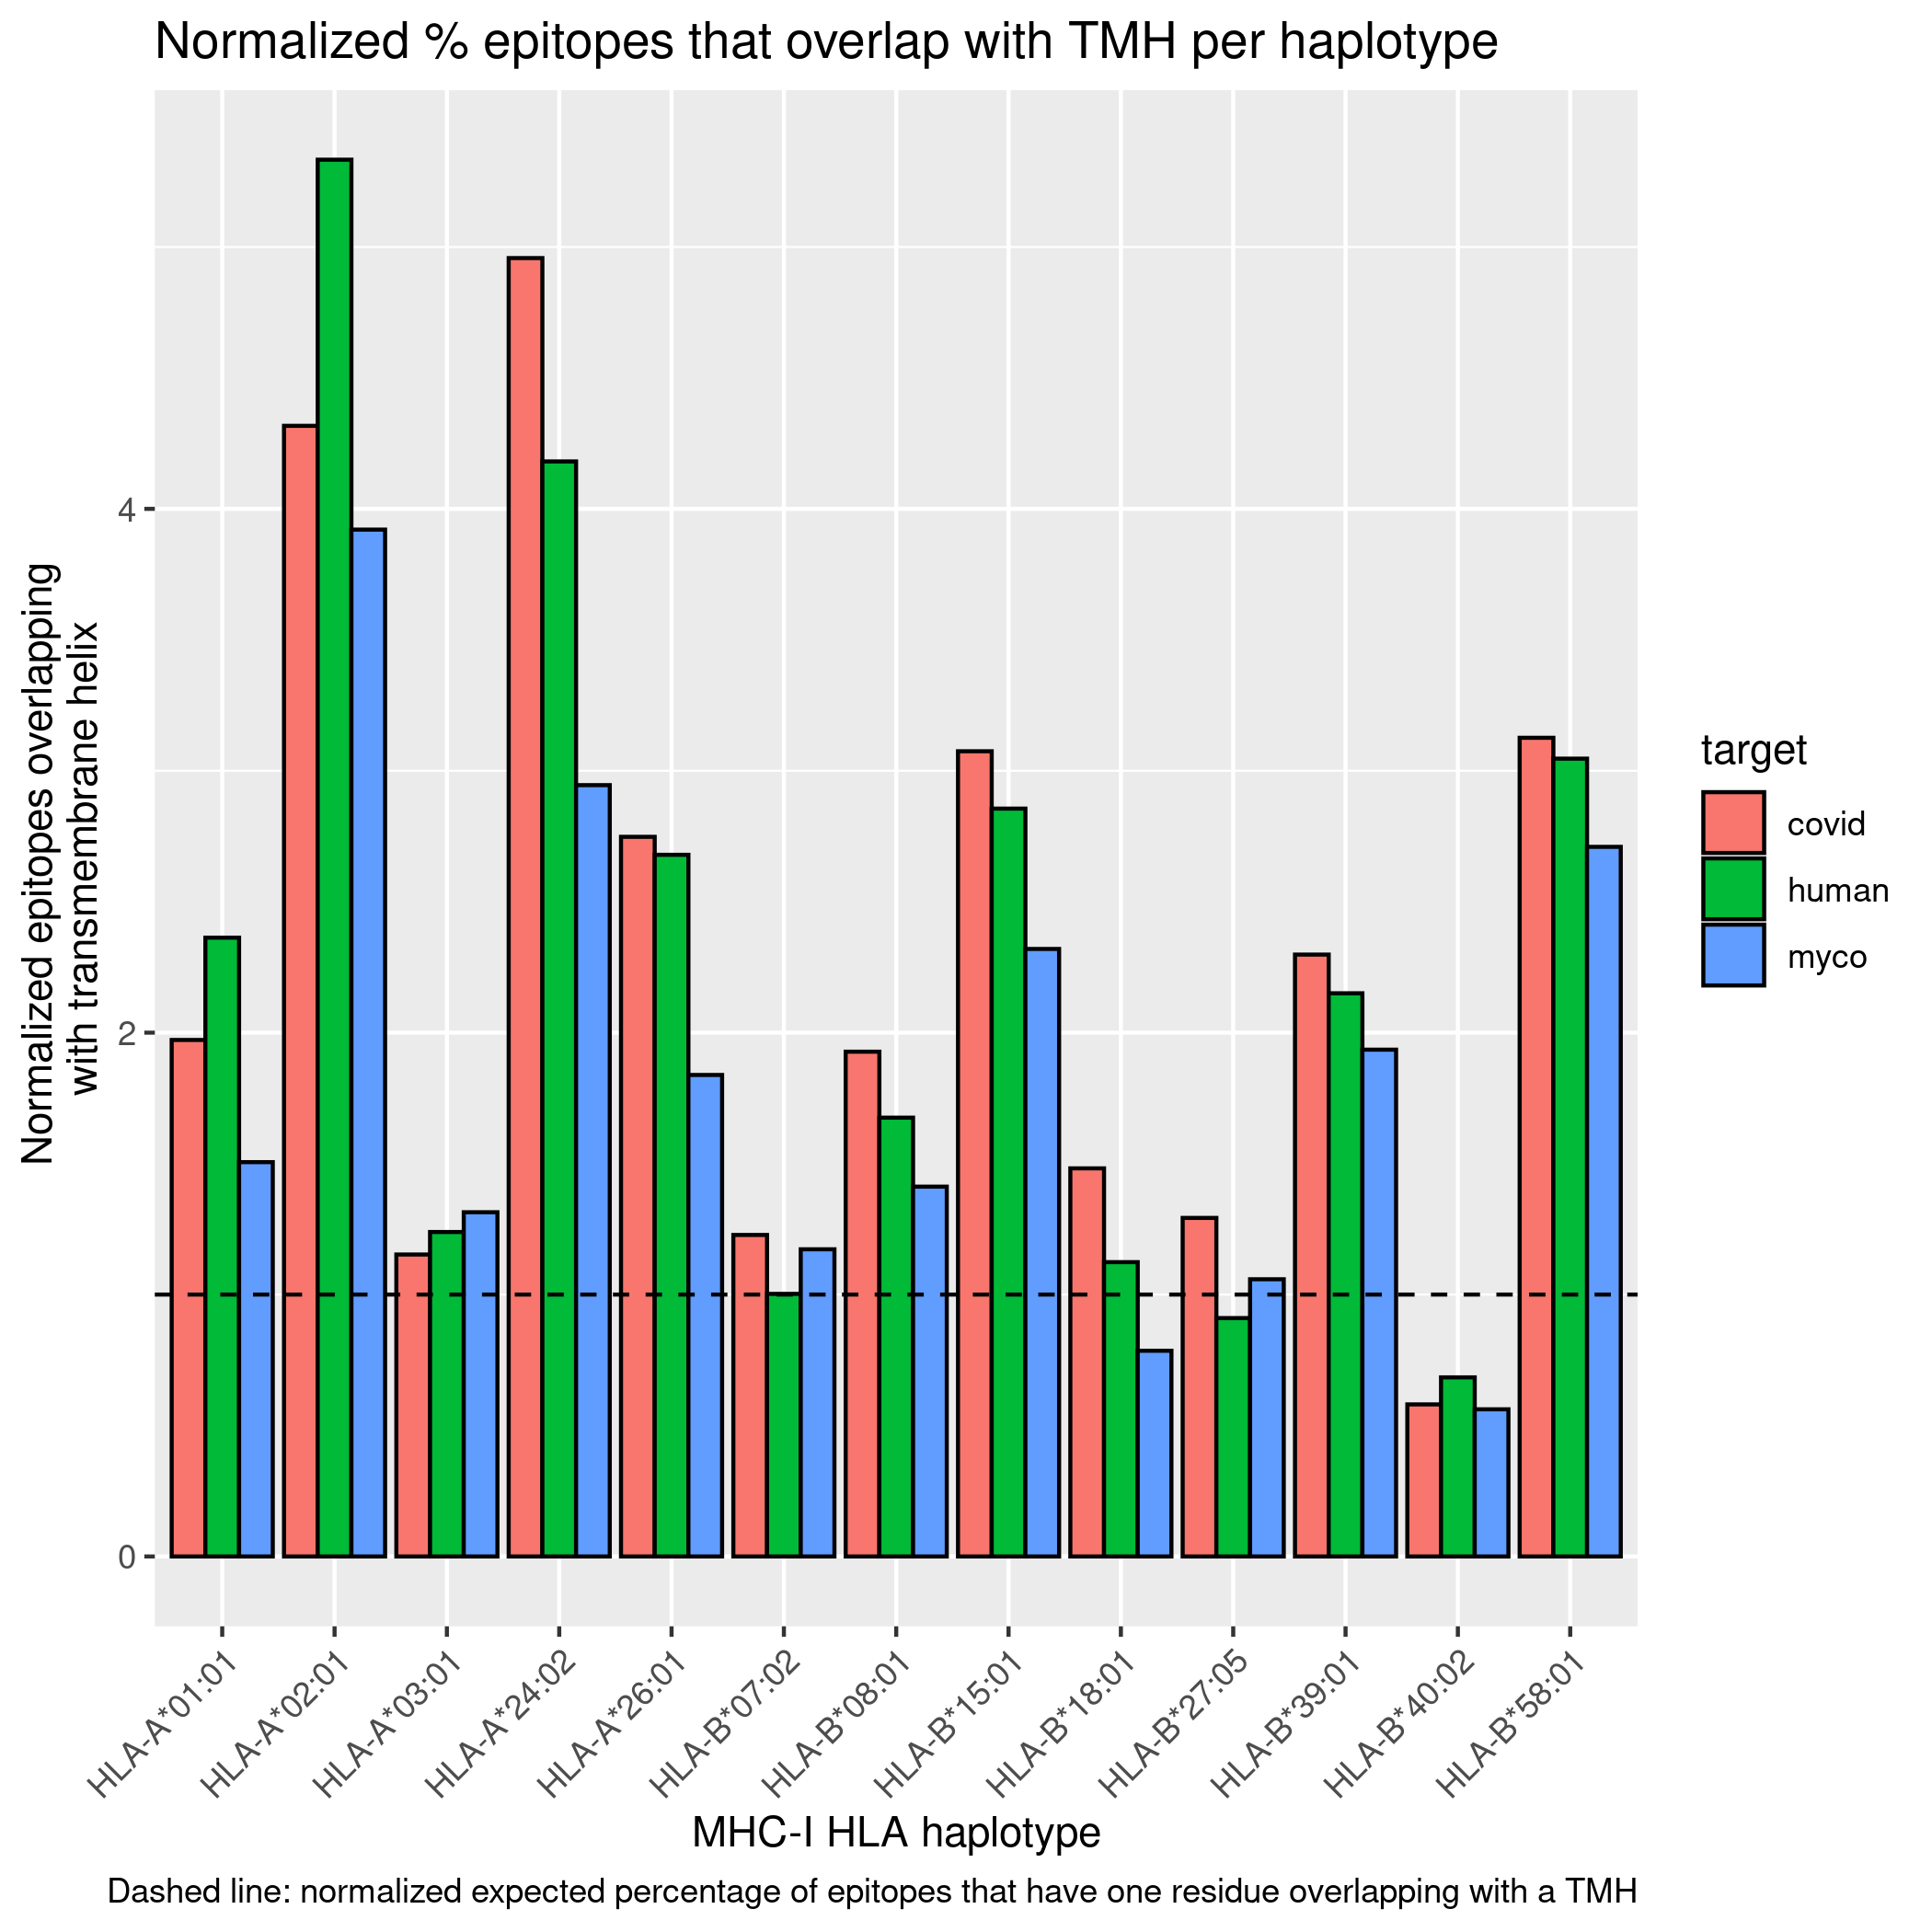
\includegraphics[width=\textwidth]{bbbq_1_smart_results/fig_f_tmh_mhc1_2_normalized.png}
  \caption{
    Normalized proportion of MHC-I epitopes overlapping with TMHs
    for human, viral and bacterial proteomes.
    Legend: covid = SARS-CoV-2,
    human = homo sapiens, myco = Mycobacterium tuberculosis
  }
  \label{fig:f_tmh_mhc1_normalized}
\end{figure}

\begin{figure}[!htbp]
  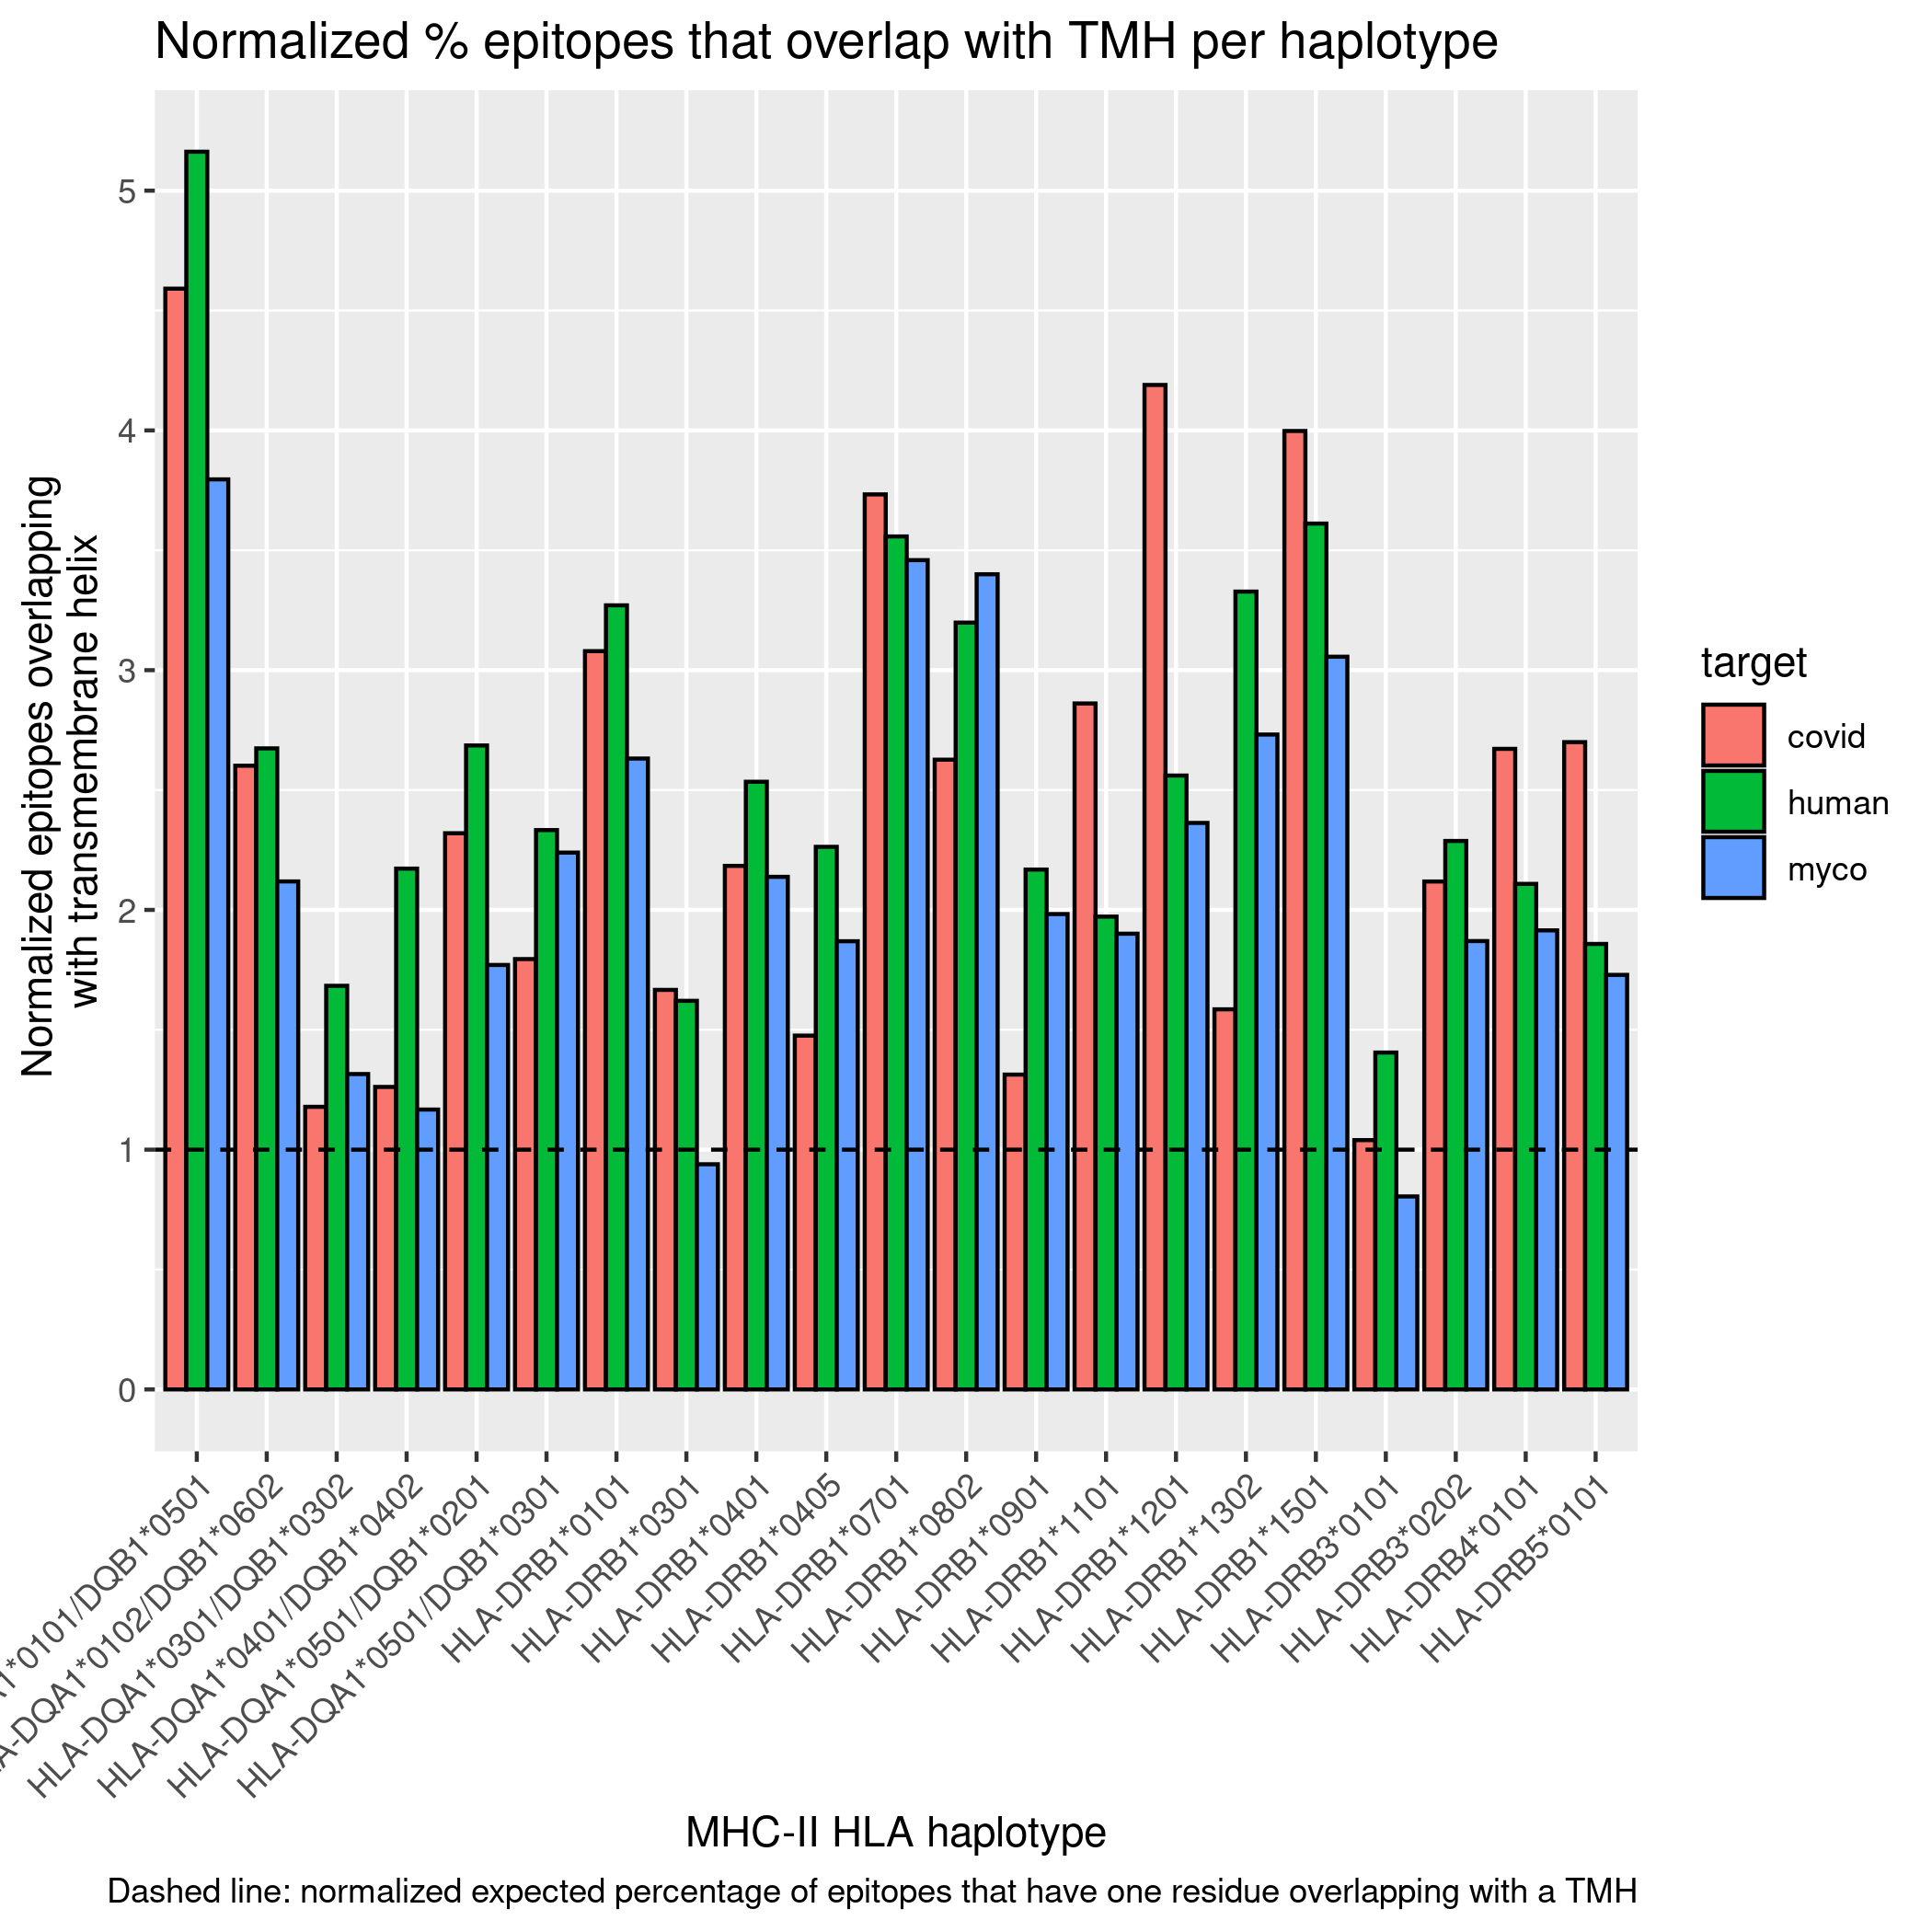
\includegraphics[width=\textwidth]{bbbq_1_smart_results/fig_f_tmh_mhc2_2_normalized.png}
  \caption{
    Normalized proportion of MHC-II epitopes overlapping with TMHs
    for human, viral and bacterial proteomes.
    Legend: covid = SARS-CoV-2,
    human = homo sapiens, myco = Mycobacterium tuberculosis
  }
  \label{fig:f_tmh_mhc2_normalized}
\end{figure}

To determine the additional over-presentation of TMH-derived epitopes 
in MHC-II (as compared to MHC-I), we used the same normalized percentages
and compared the averages between MHC-I and MHC-II.
Figure \ref{fig:rel_presentation_per_haplotype} shows the normalized
TMH-derived epitope presentation per haplotype.
To compare the TMH-derived over-presentation per MHC class, 
we plot the mean and standard error of the normalized values,
grouped per haplotype in figure \ref{fig:rel_presentation}.

\begin{figure}[!htbp]
  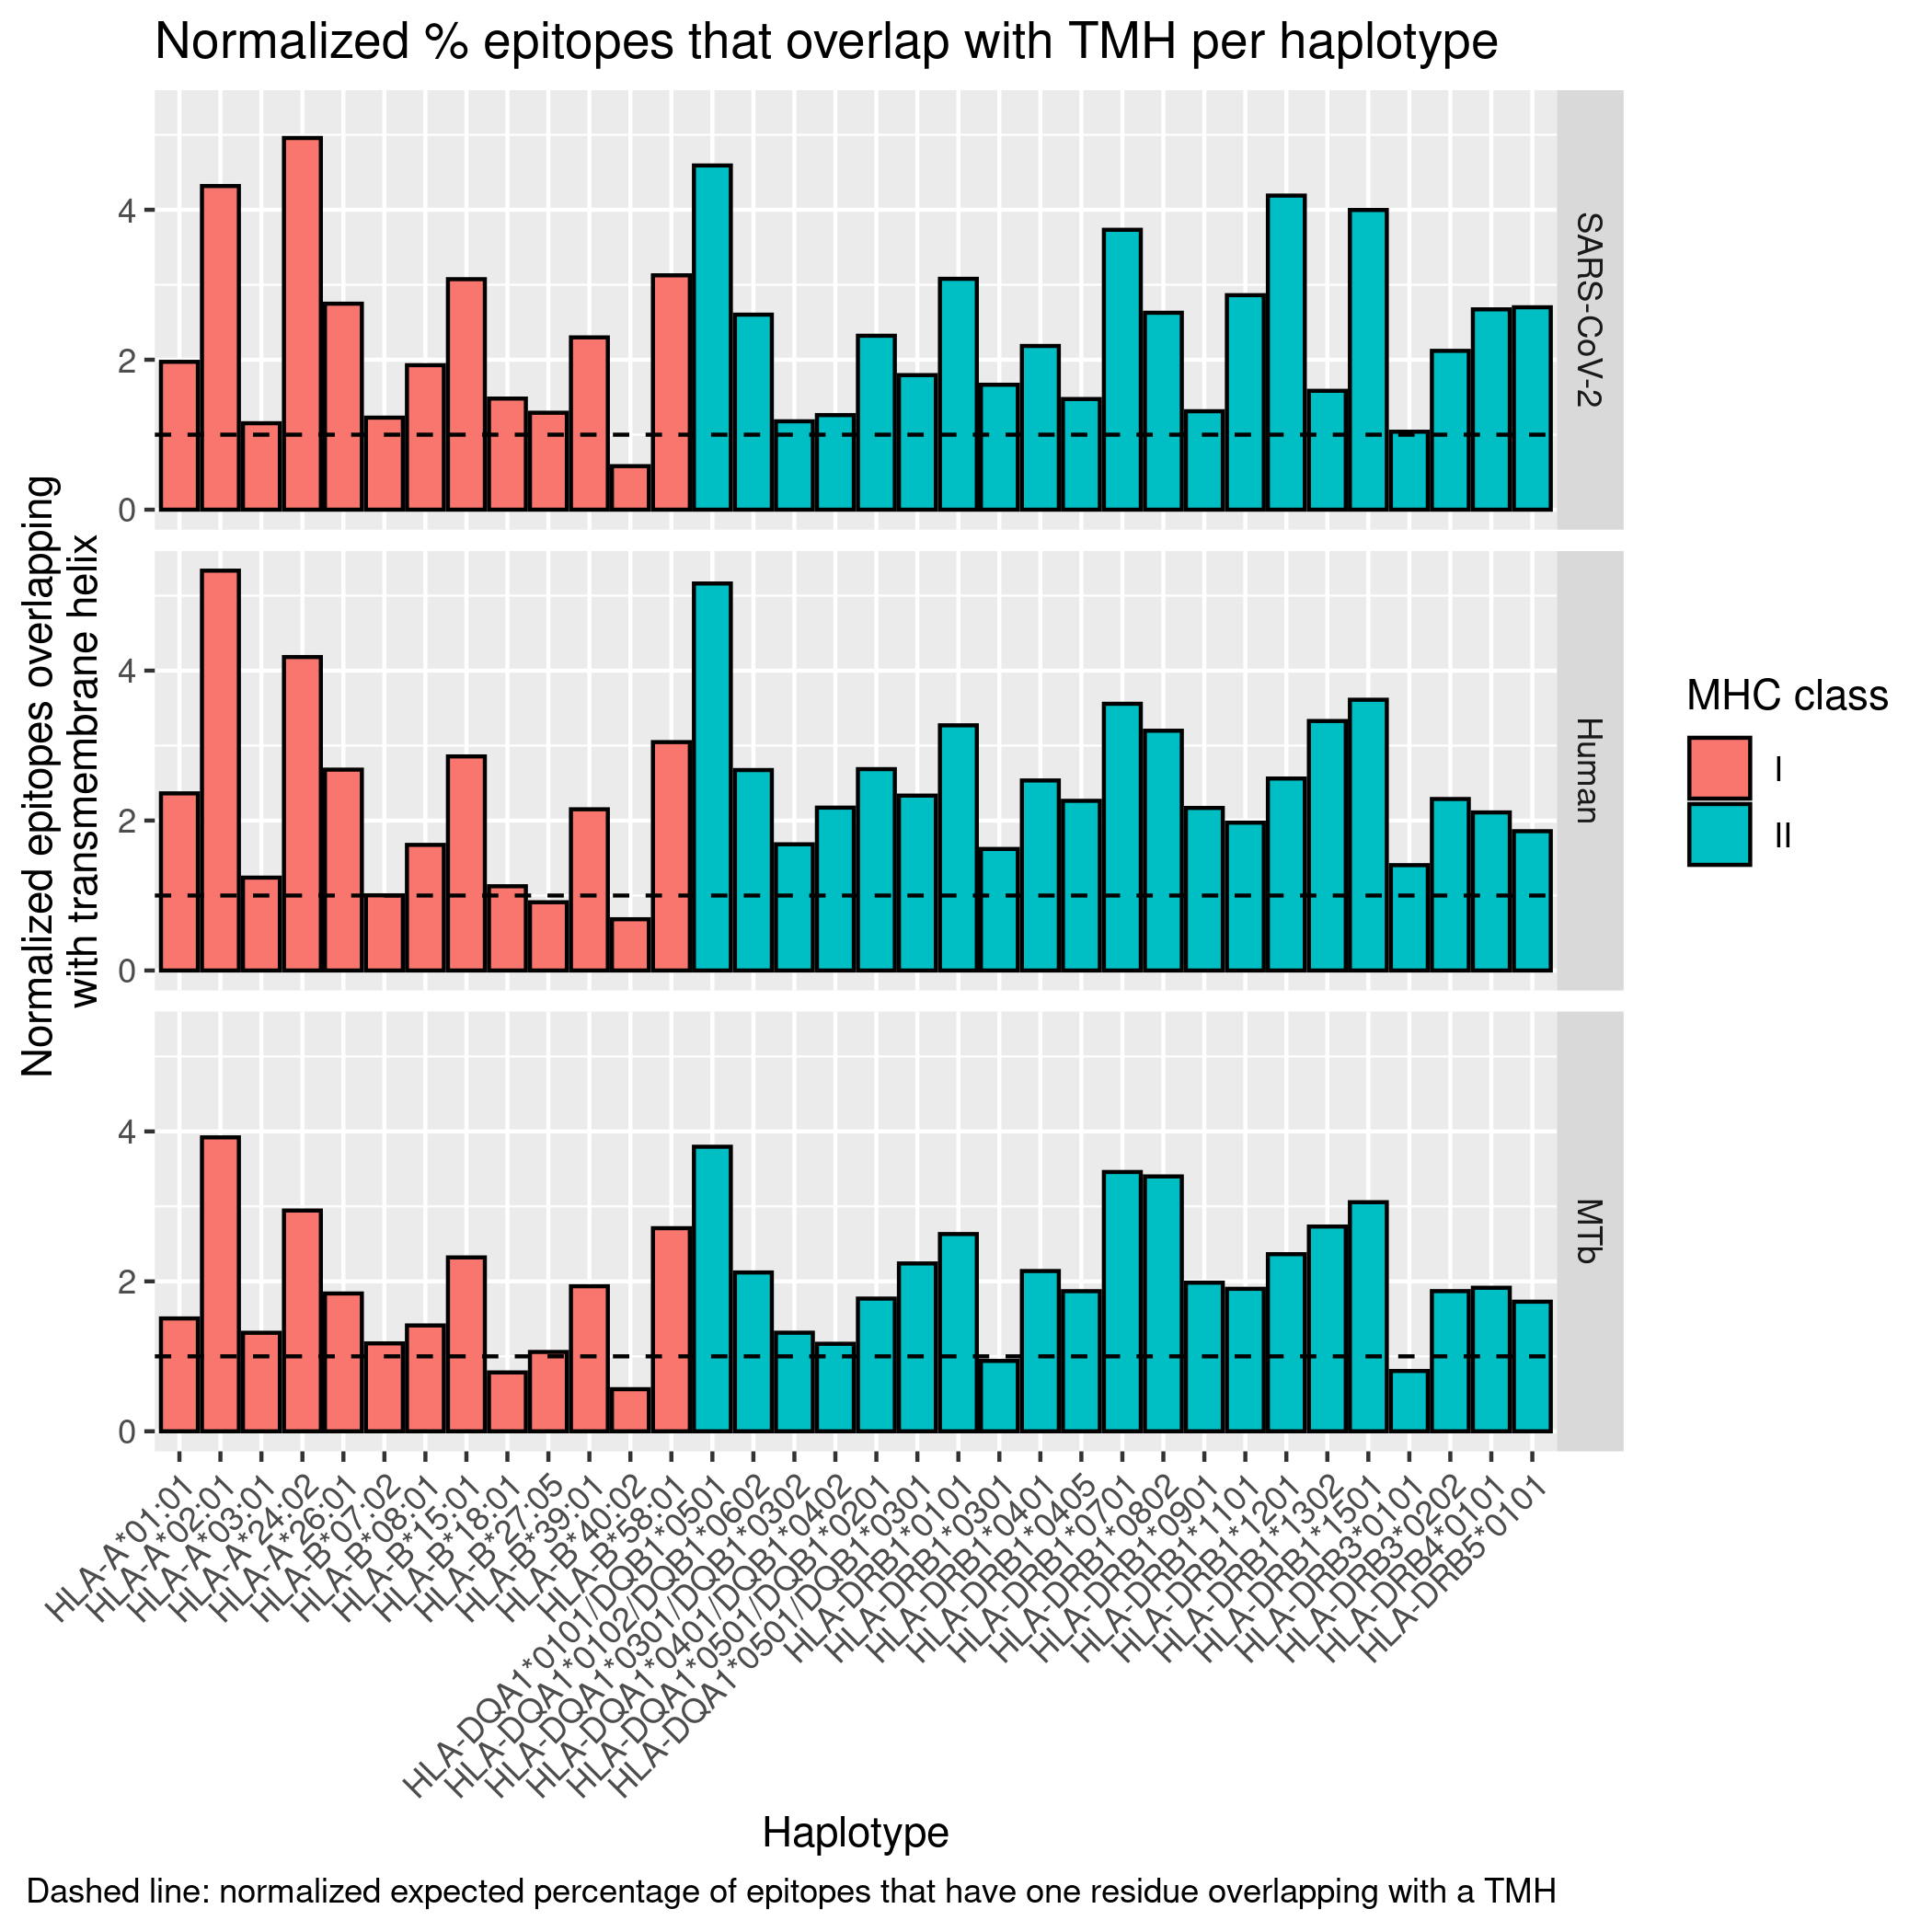
\includegraphics[width=\textwidth]{bbbq_1_smart_results/fig_rel_presentation_per_haplotype.png}
  \caption{
    Normalized proportion of MHC-I and MHC-II epitopes overlapping with TMHs,
    for the different haplotypes and proteomes
  }
  \label{fig:rel_presentation_per_haplotype}
\end{figure}

\begin{figure}[!htbp]
  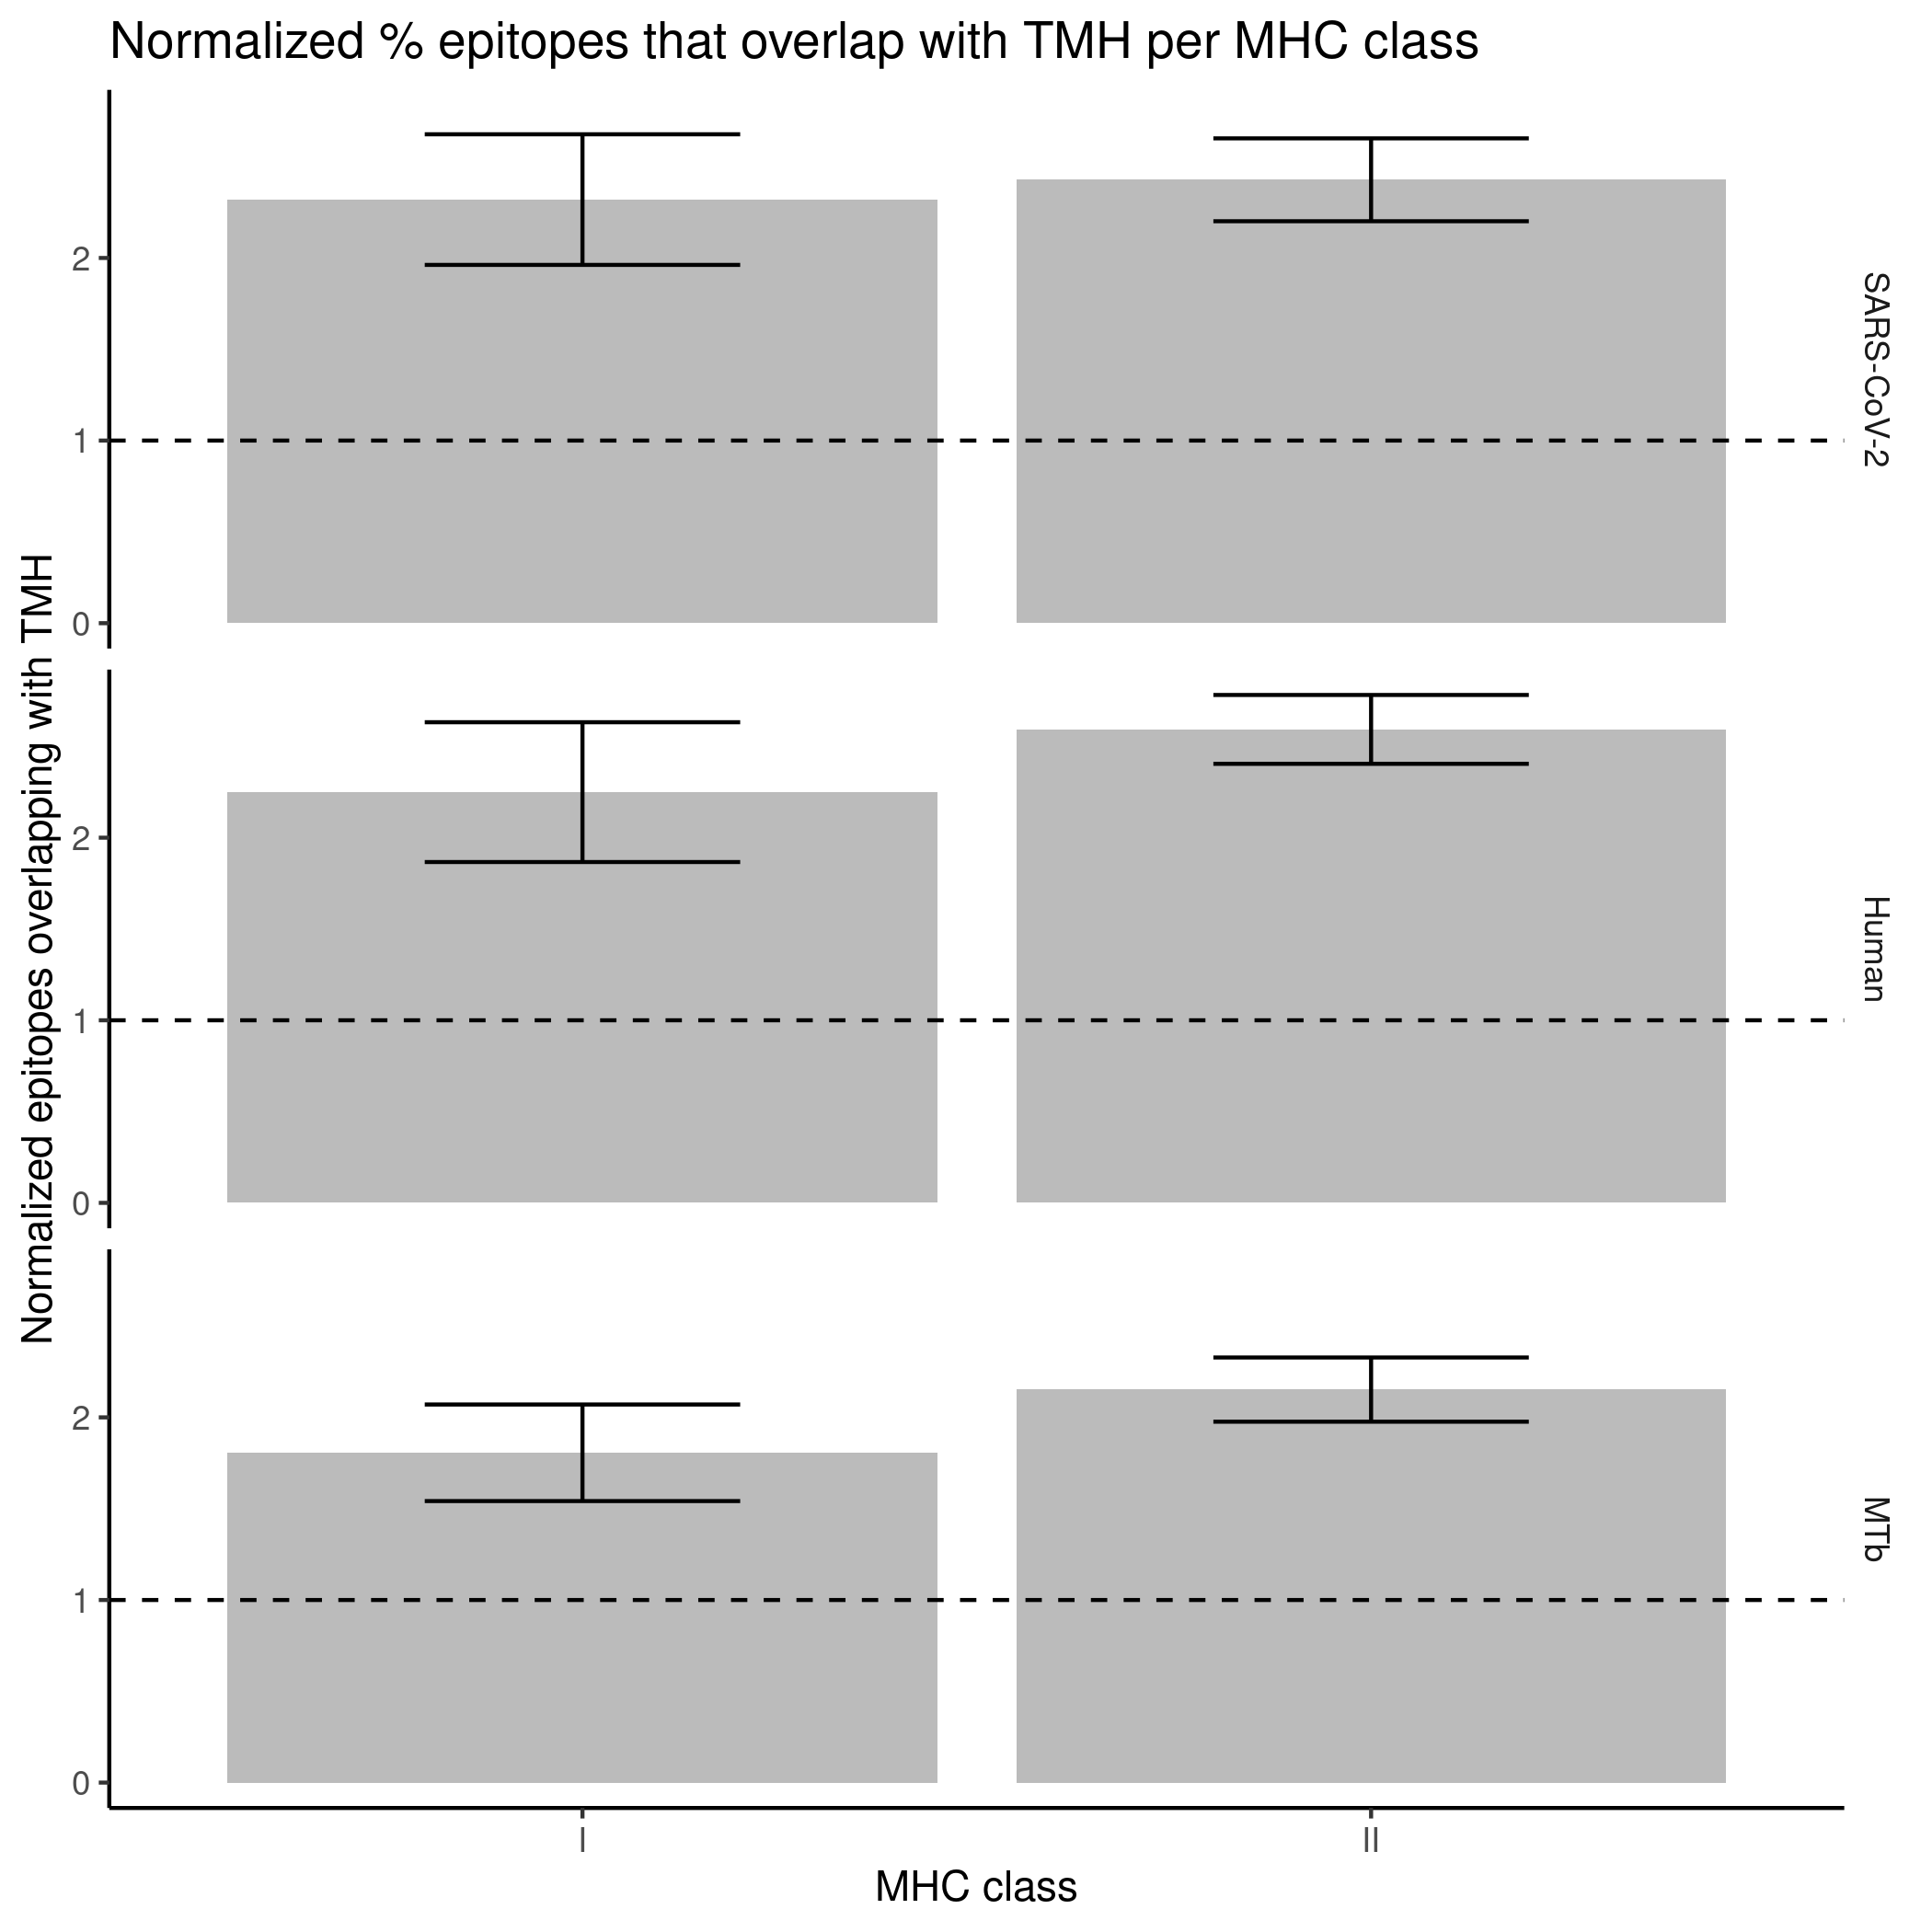
\includegraphics[width=\textwidth]{bbbq_1_smart_results/fig_rel_presentation.png}
  \caption{
    Normalized proportion of MHC-I and MHC-II epitopes overlapping with TMHs,
    for the different MHC classes and proteomes. Error bars denote the
    standard error.
  }
  \label{fig:rel_presentation}
\end{figure}

%%%%%%%%%%%%%%%%%%%%%%%%%%%%%%%%%%%%%%%%%%%%%%%%%%%%%%%%%%%%%%%%%%%%%%%%%%%%%%%%
\subsection{Evolutionary conservation}
%%%%%%%%%%%%%%%%%%%%%%%%%%%%%%%%%%%%%%%%%%%%%%%%%%%%%%%%%%%%%%%%%%%%%%%%%%%%%%%%

See tables \ref{tab:ncbi_counts_1} and tables \ref{tab:ncbi_counts_2}
for an overview of all amounts.
In table \ref{tab:ncbi_counts_1} one expects [RJCB: name these]
numbers to add up. 
The number of unique SNPs and unique gene names
does not add up for MAP and TMP,
as one SNP may work on multiple isoforms, some of which can be MAP
where others can be TMP.
The number of unique SNPs and unique gene names
does not add up for TMPs in TMH and TMP in soluble regions
as one SNP may work on multiple isoforms, some of which can be MAP
where others can be TMP, and some SNPs fall in a TMH, where others
are found in soluble regions
In table \ref{tab:ncbi_counts_2} one expects [RJCB: name these]
numbers to add up. 


% Label: tab:ncbi_counts_1
\begin{table}

\caption{\label{tab:ncbi_counts_1}Amounts. raw = all variations, including DNA variations. all\_proteins = all proteins. map = membrane associated protein. tmp = transmembrane protein. in\_tmh = in transmembrane helix of TMP. in\_sol = in soluble region of TMP. }
\centering
\begin{tabular}[t]{l|r|r|r|r|r|r}
\hline
what & raw & all\_proteins & map & tmp & in\_tmh & in\_sol\\
\hline
Number of variations & 60931 & 37831 & 16623 & 21208 & 3803 & 17405\\
\hline
Number of unique variations & 60544 & 37630 & 16606 & 21024 & 3789 & 17235\\
\hline
Number of unique SNPs & NA & 9621 & 4219 & 6026 & 1140 & 4936\\
\hline
Number of unique gene names & 953 & 911 & 457 & 605 & 325 & 590\\
\hline
Number of unique protein names & 5163 & 4780 & 2227 & 2553 & 1280 & 2467\\
\hline
Percentage TMH & NA & 10 & 0 & 19 & 26 & 18\\
\hline
\end{tabular}
\end{table}

% Label: tab:ncbi_counts_2
\begin{table}

\caption{\label{tab:ncbi_counts_2}Amounts. single\_in\_tmh = in transmembrane helix of single-spanner. single\_in\_sol = in soluble region of single-spanner. multi\_in\_tmh = in transmembrane helix of multi-spanner. multi\_in\_sol = in soluble region of multi-spanner. }
\centering
\begin{tabular}[t]{l|r|r|r|r}
\hline
what & single\_in\_tmh & single\_in\_sol & multi\_in\_tmh & multi\_in\_sol\\
\hline
Number of variations & 452 & 7734 & 3351 & 9671\\
\hline
Number of unique variations & 451 & 7733 & 3338 & 9502\\
\hline
Number of unique SNPs & 160 & 2393 & 994 & 2762\\
\hline
Number of unique gene names & 96 & 282 & 243 & 344\\
\hline
Number of unique protein names & 304 & 1032 & 976 & 1435\\
\hline
Percentage TMH & 11 & 5 & 35 & 26\\
\hline
\end{tabular}
\end{table}

Figure \ref{fig:snps_per_gene_name_ncbi} shows the distribution of the
number of SNPs per gene name, at 2020-12-14.

\begin{figure}[!htbp]
  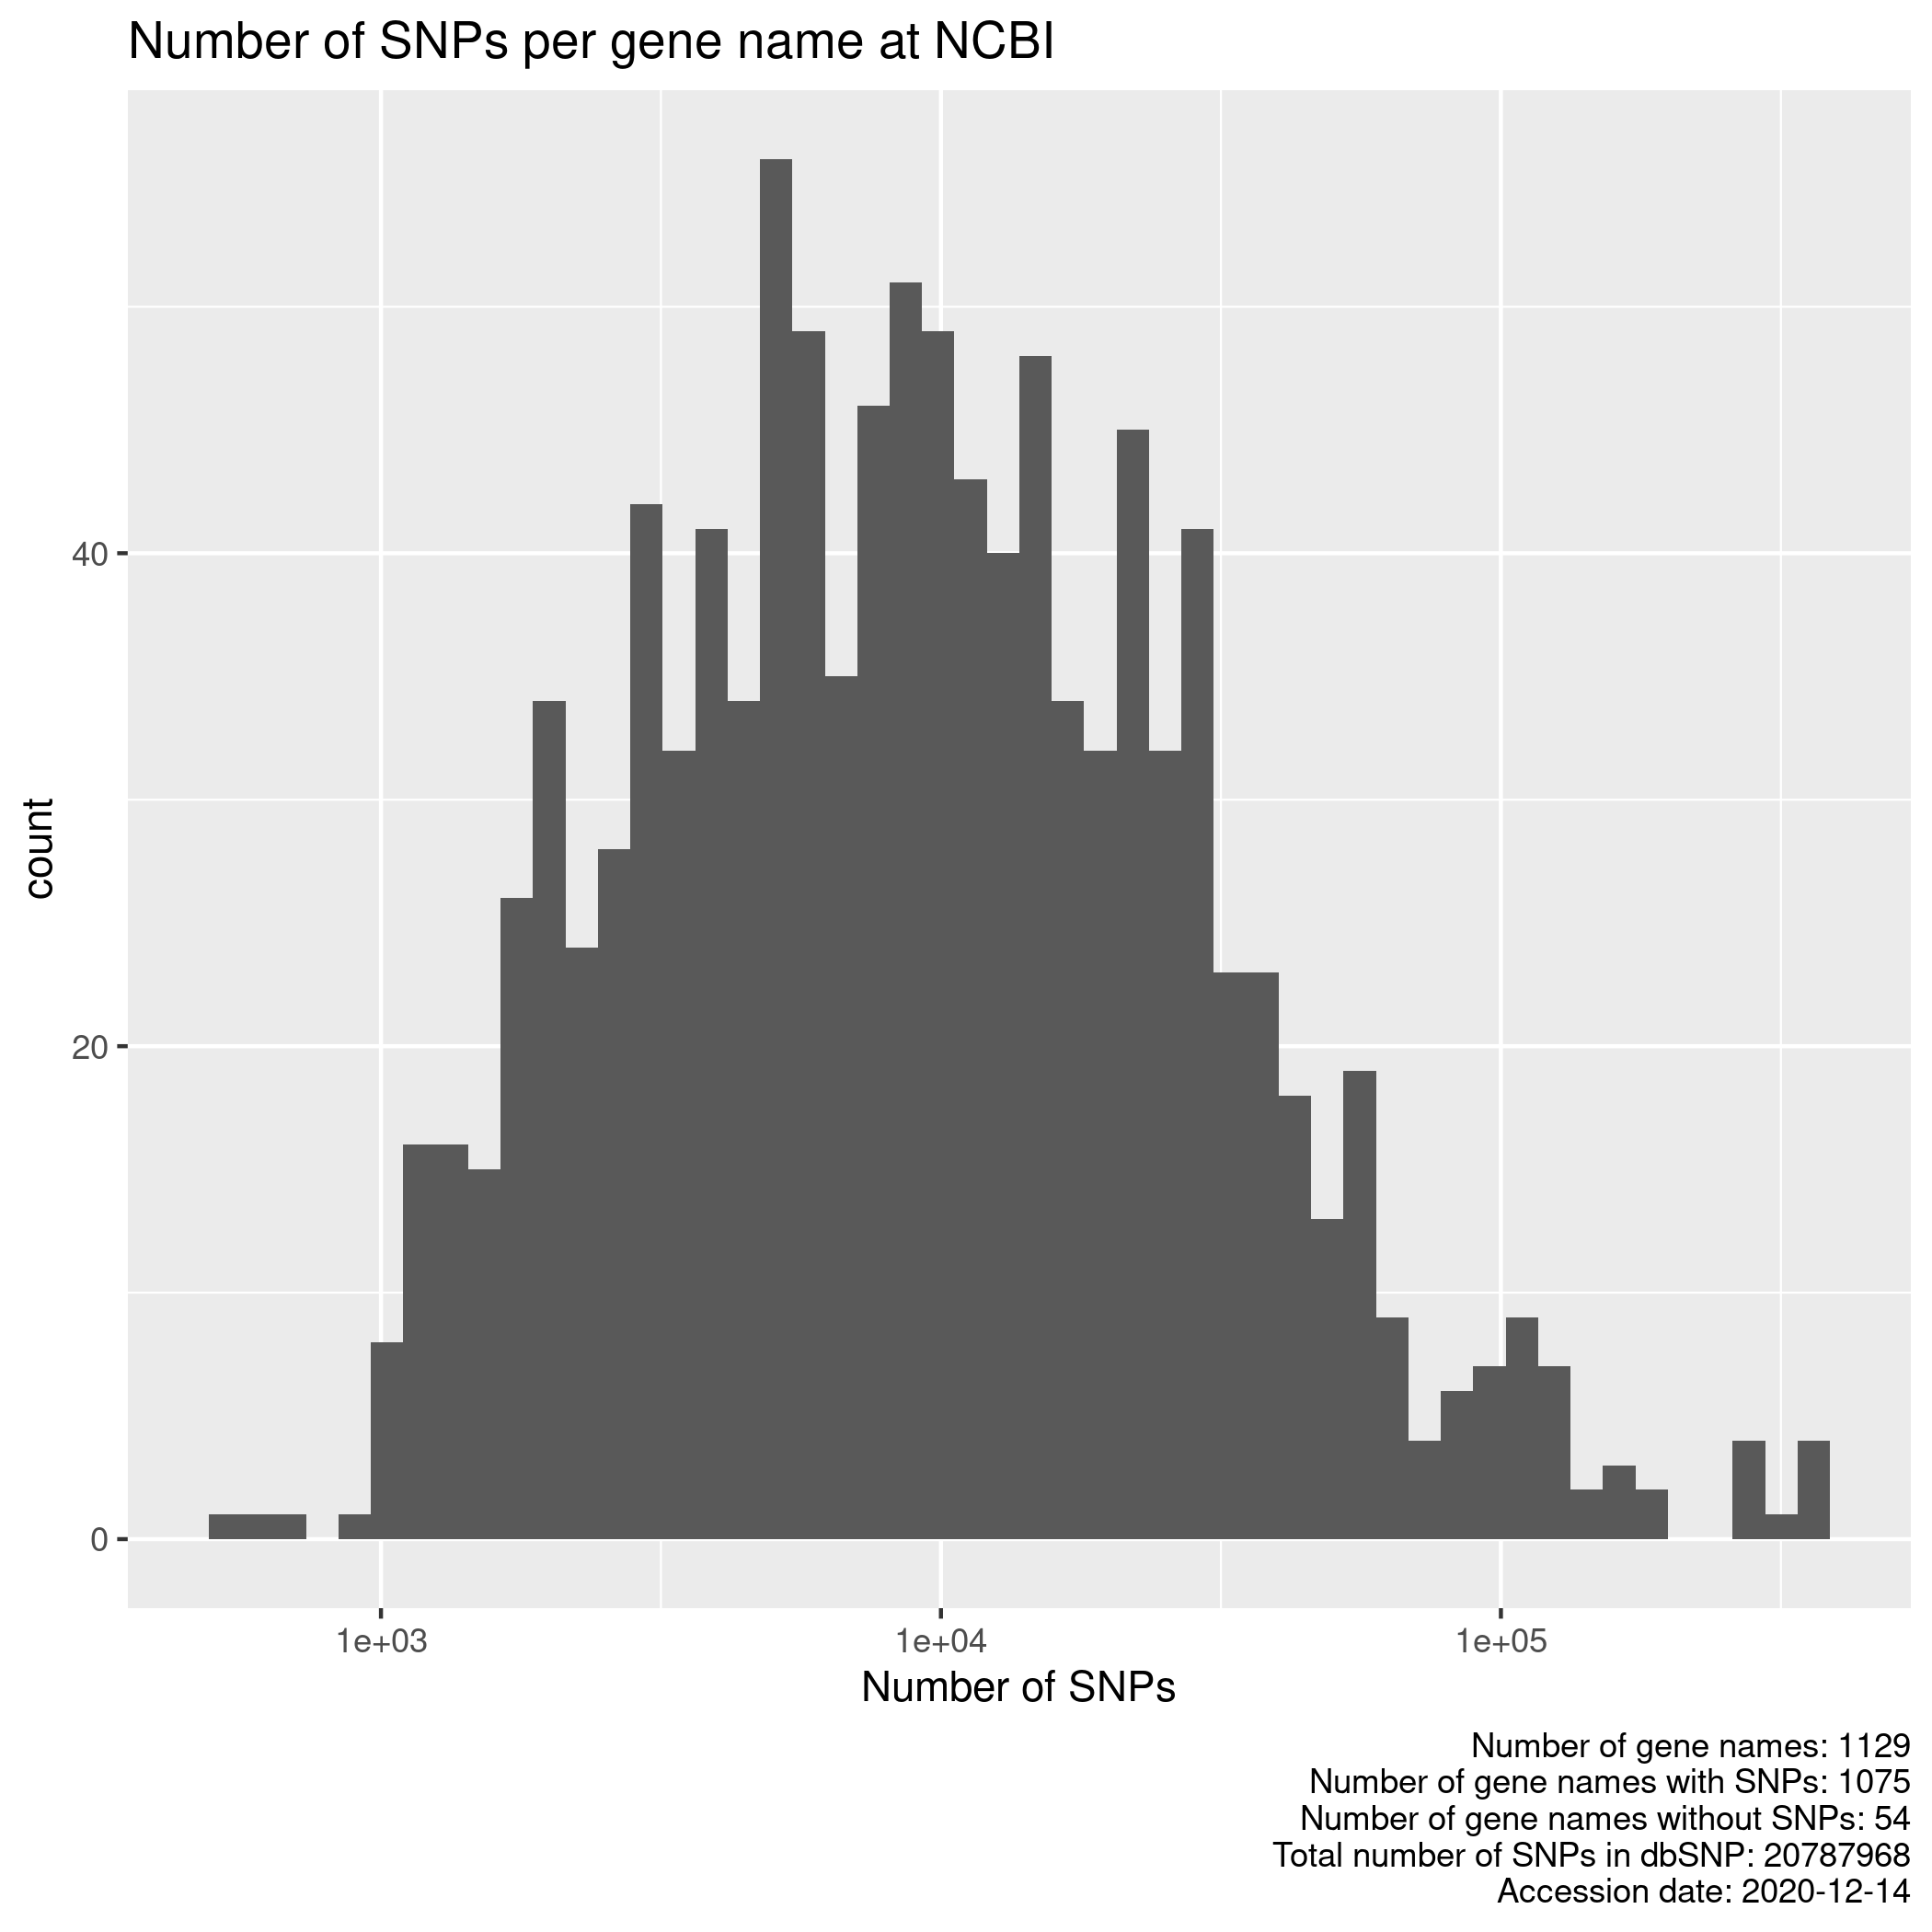
\includegraphics[width=\textwidth]{ncbi_peregrine_results/fig_snps_per_gene_name_ncbi.png}
  \caption{
    Distribution of the number of SNPs per gene name in the NCBI database.
  }
  \label{fig:snps_per_gene_name_ncbi}
\end{figure}

\begin{figure}[!htbp]
  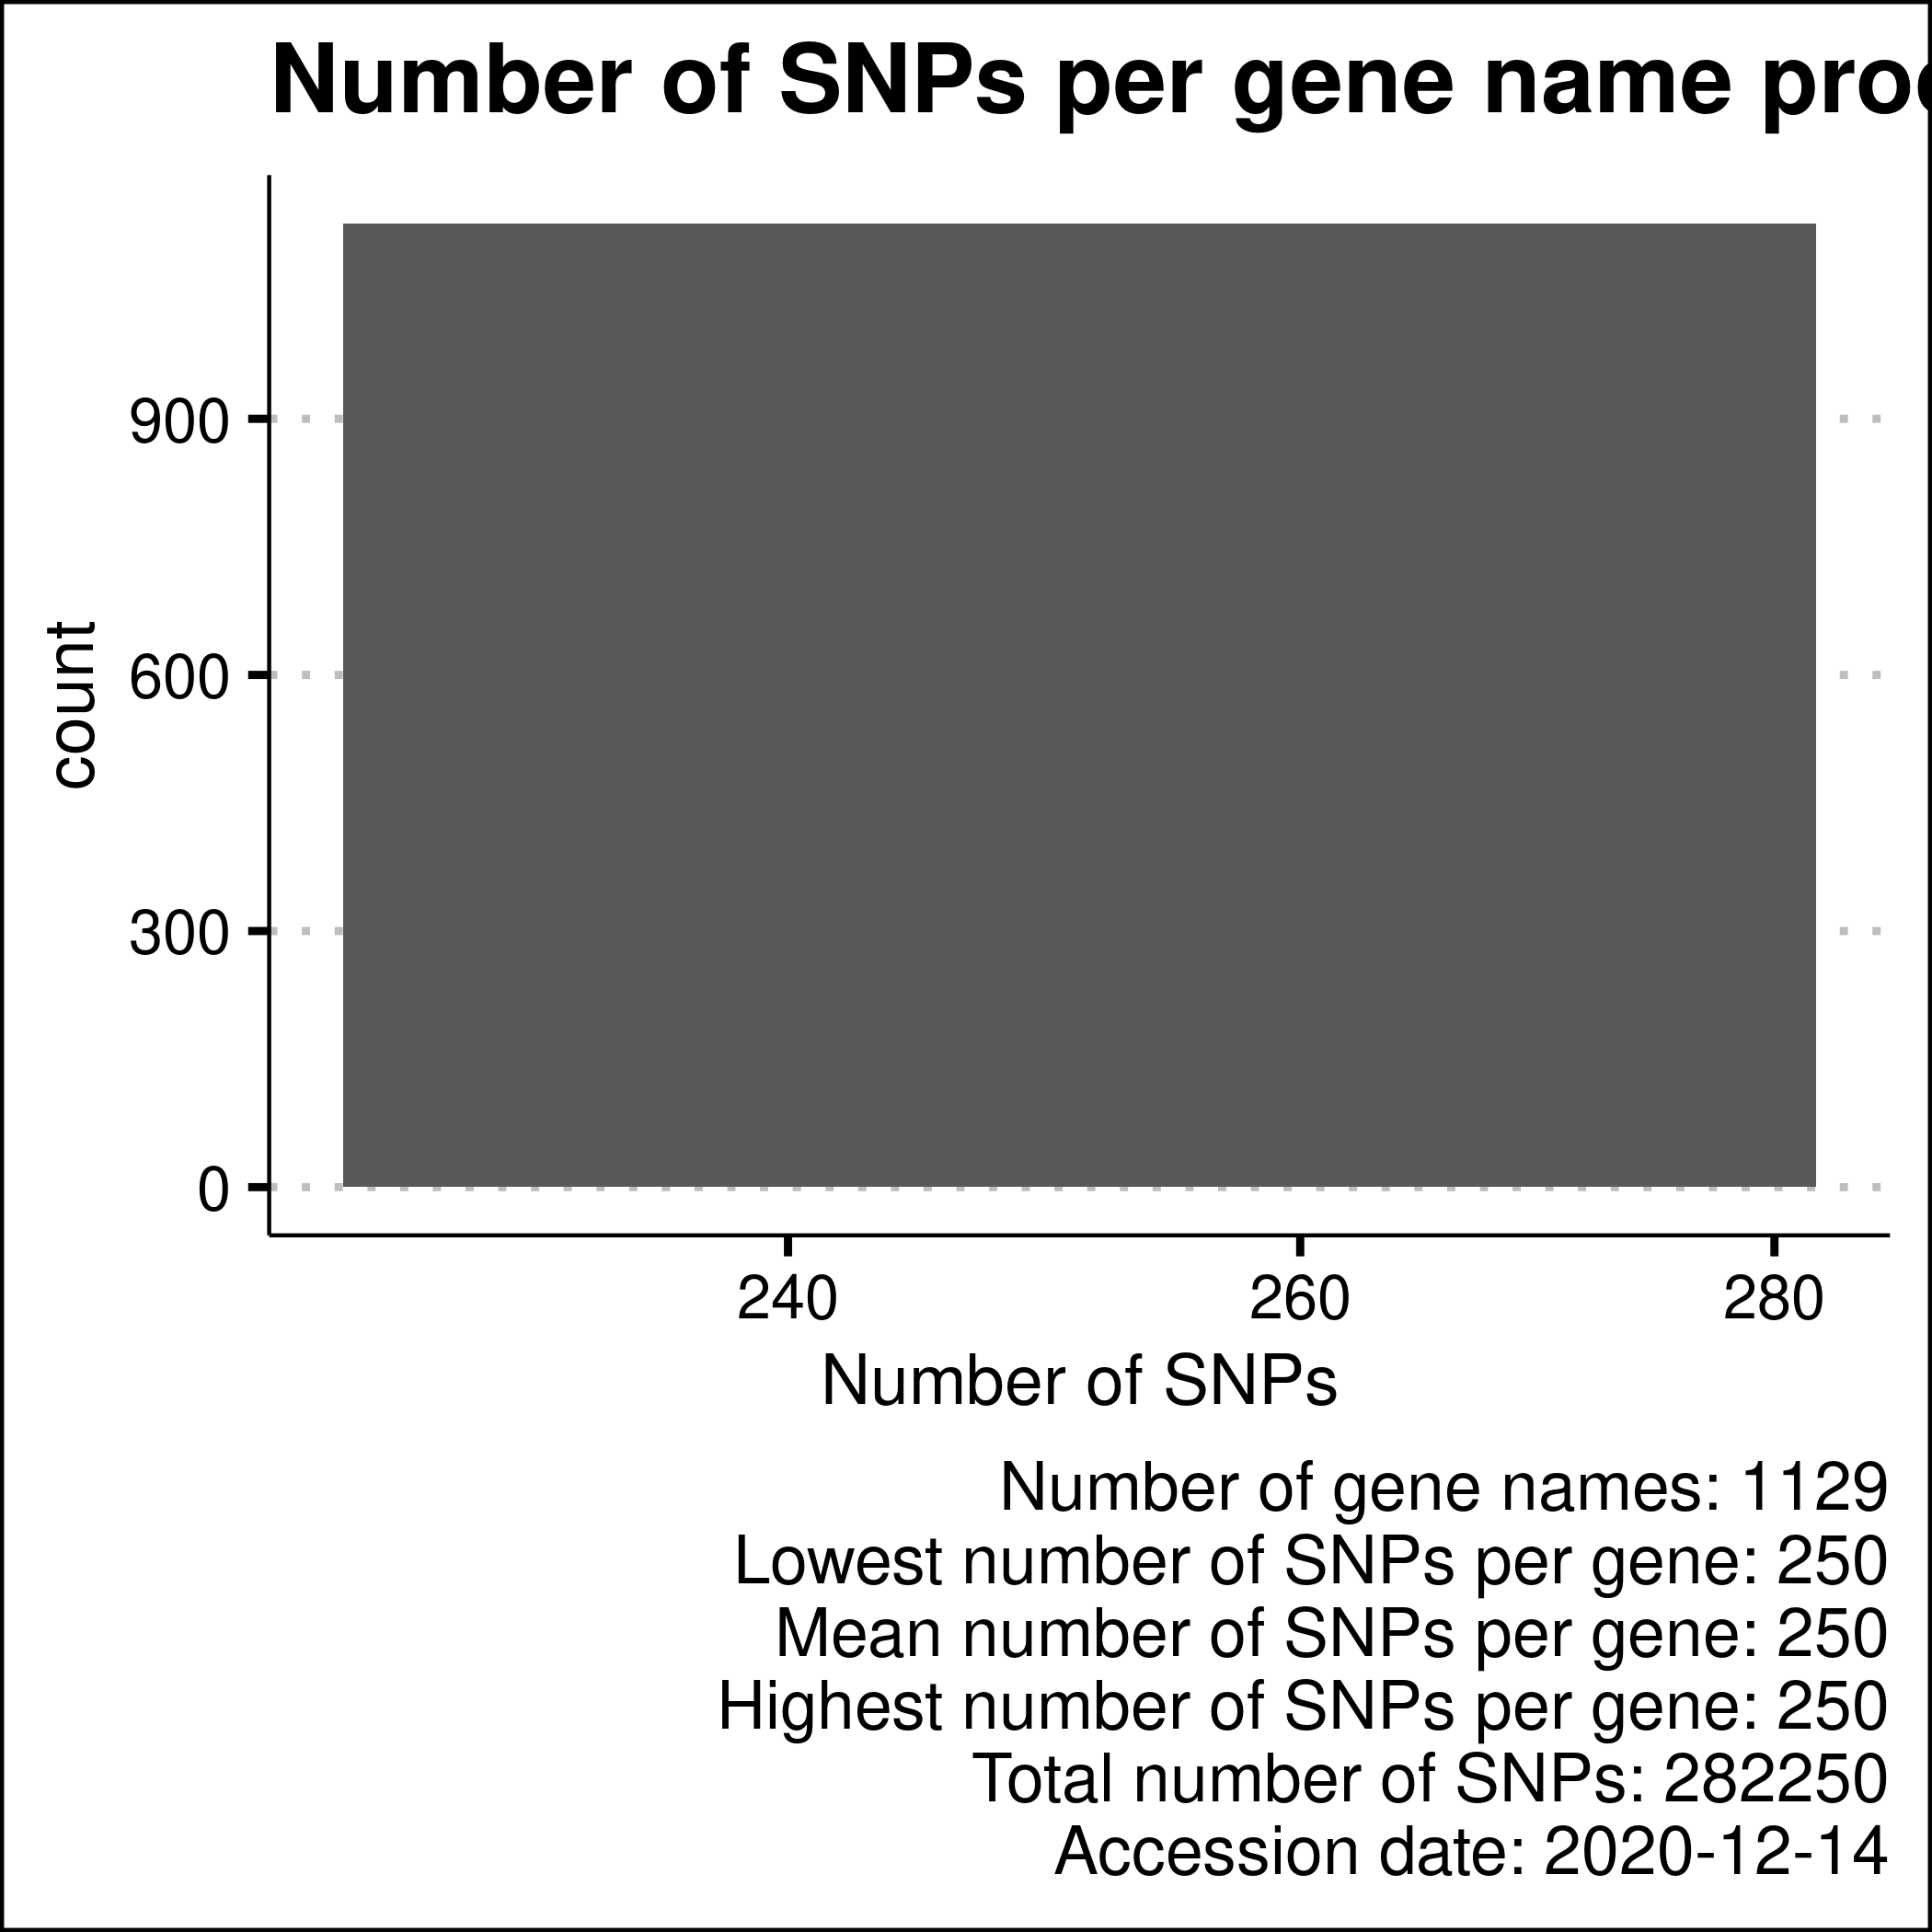
\includegraphics[width=\textwidth]{ncbi_peregrine_results/fig_snps_per_gene_name_processed.png}
  \caption{
    Distribution of the number of protein variations and SNPs per gene name processed.
  }
  \label{fig:snps_per_gene_name_processed}
\end{figure}

%Figure \ref{fig:f_tmh_ncbi} shows the distribution 
%of the percentages of TMH of transmembrane proteins.
%
%\begin{figure}[!htbp]
%  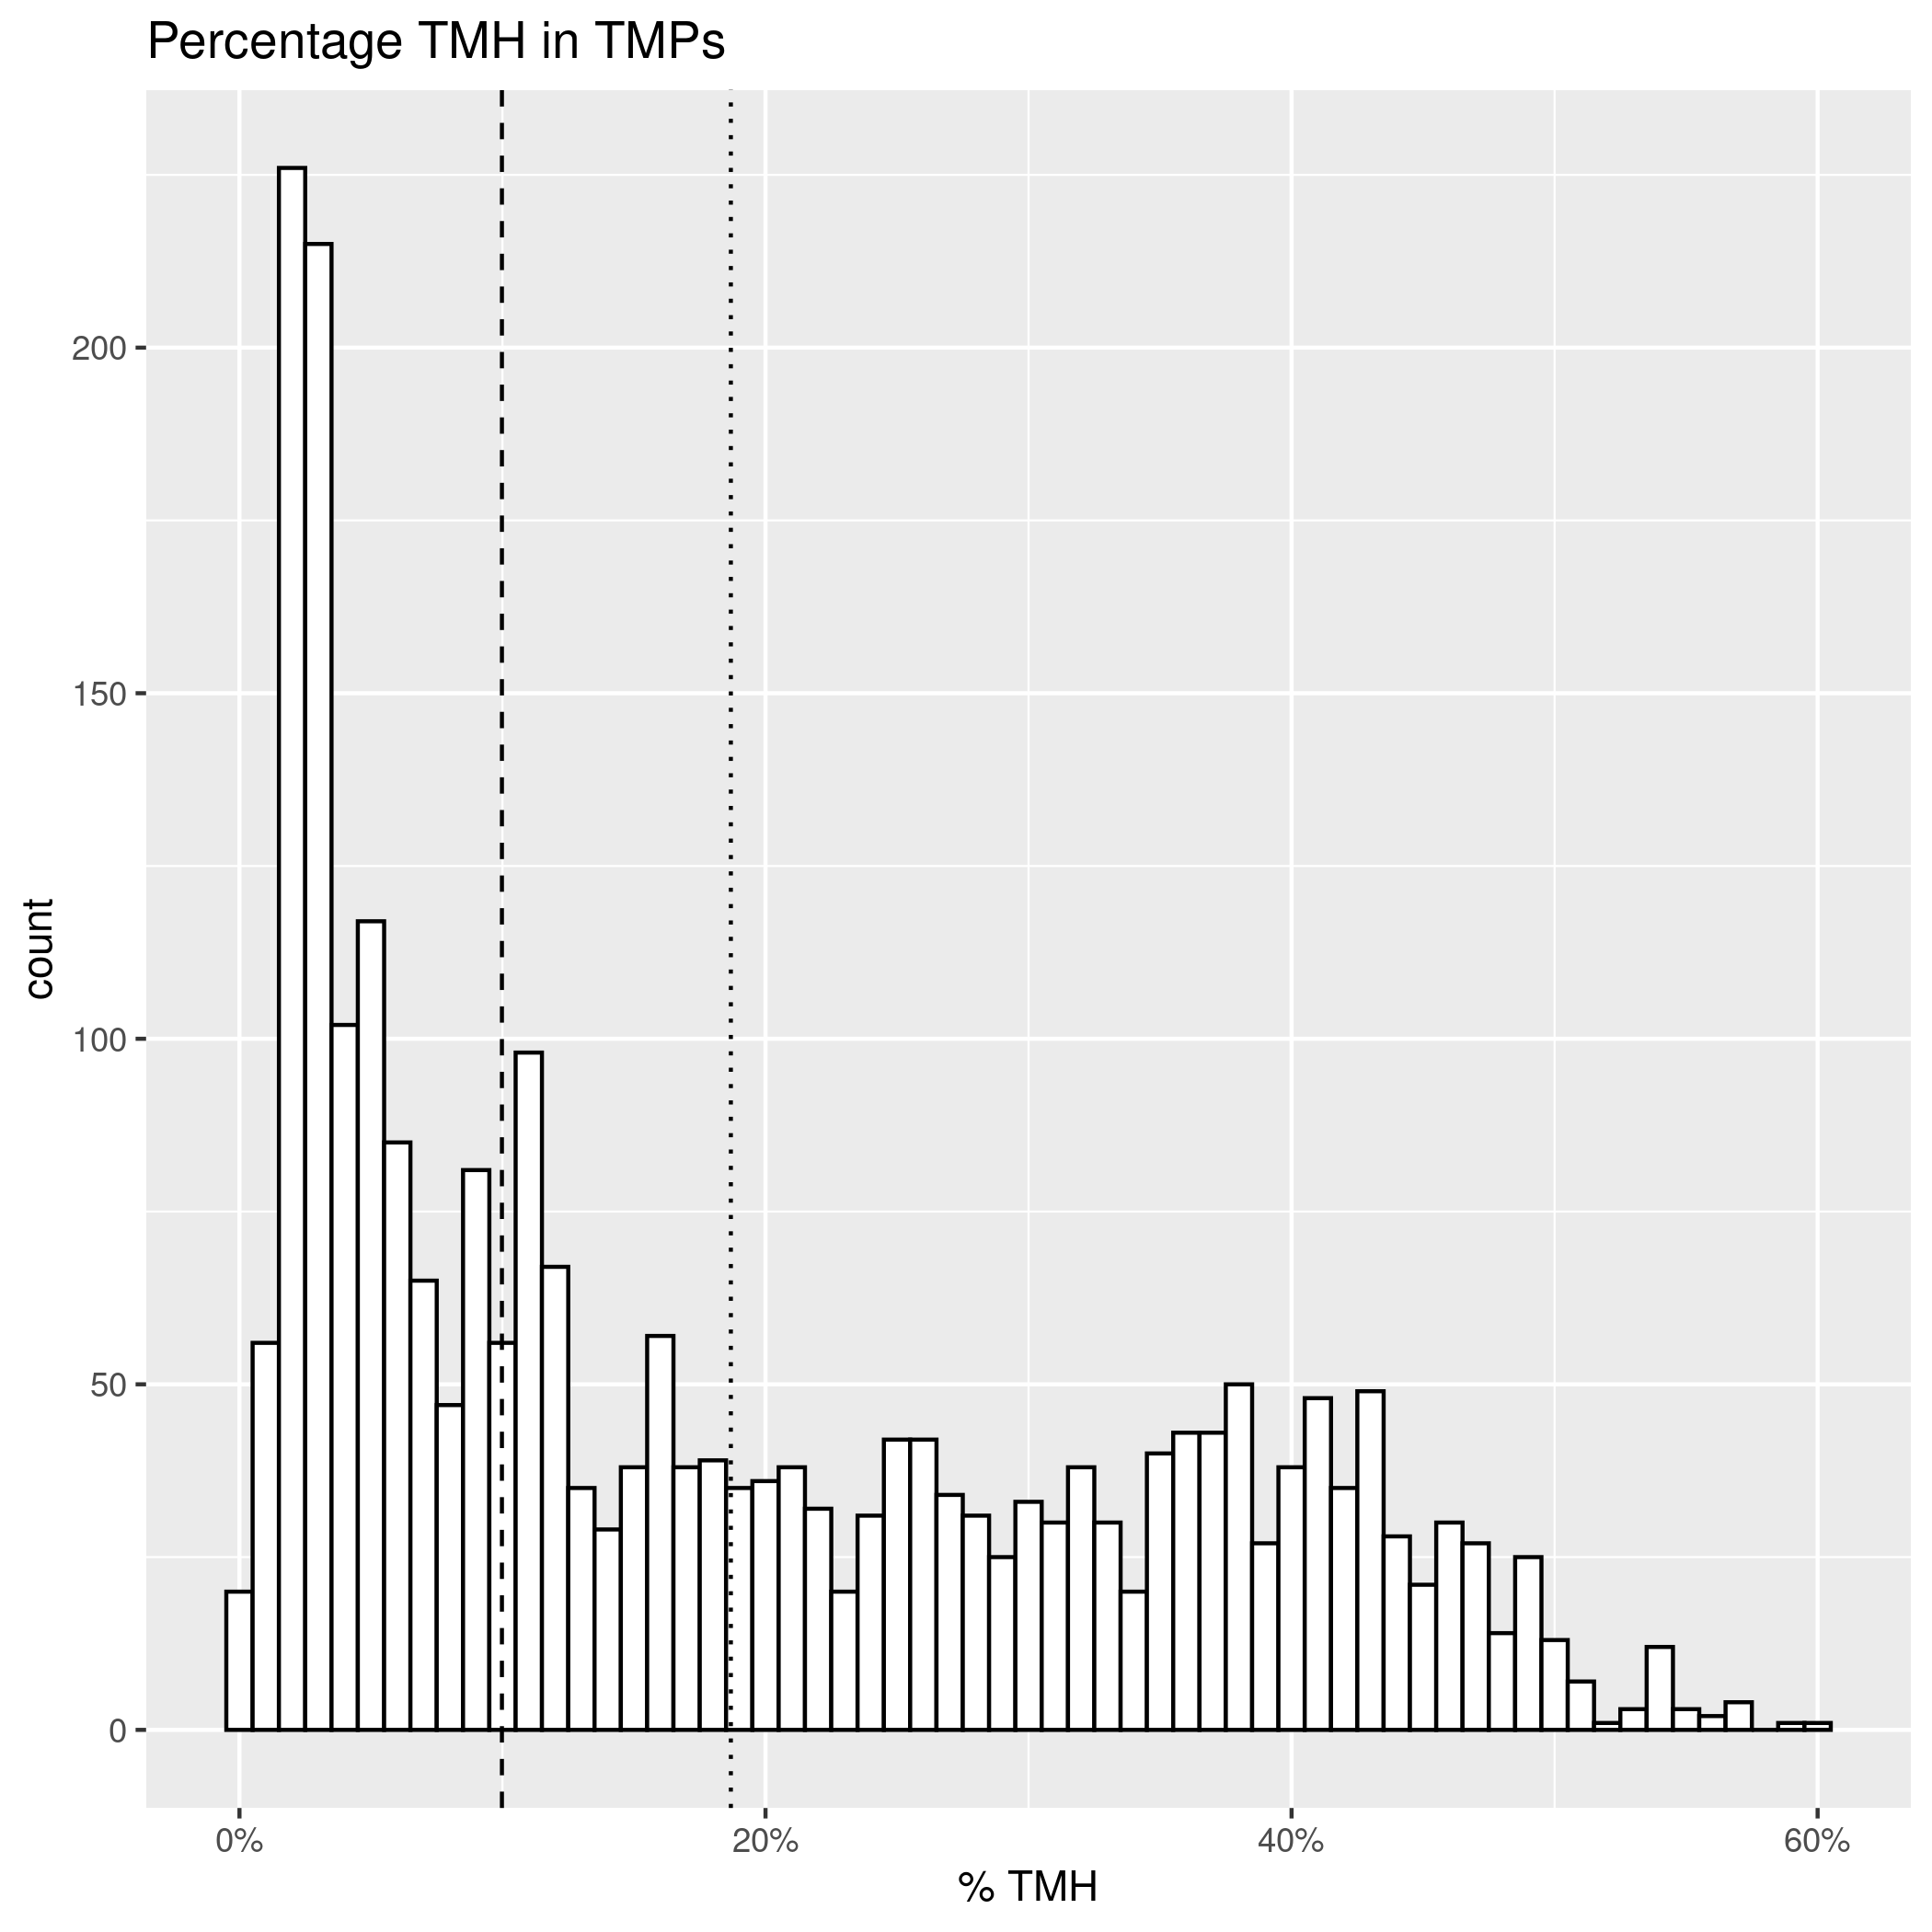
\includegraphics[width=\textwidth]{ncbi_peregrine_results/fig_f_tmh_ncbi.png}
%  \caption{
%    Distribution of the percentages of TMH of transmembrane proteins.
%    Dashed vertical line: mean \% TMH in all proteins.
%    Dotted vertical line: mean \% TMH in TMPs.
%  }
%  \label{fig:f_tmh_ncbi}
%\end{figure}

\begin{figure}[!htbp]
  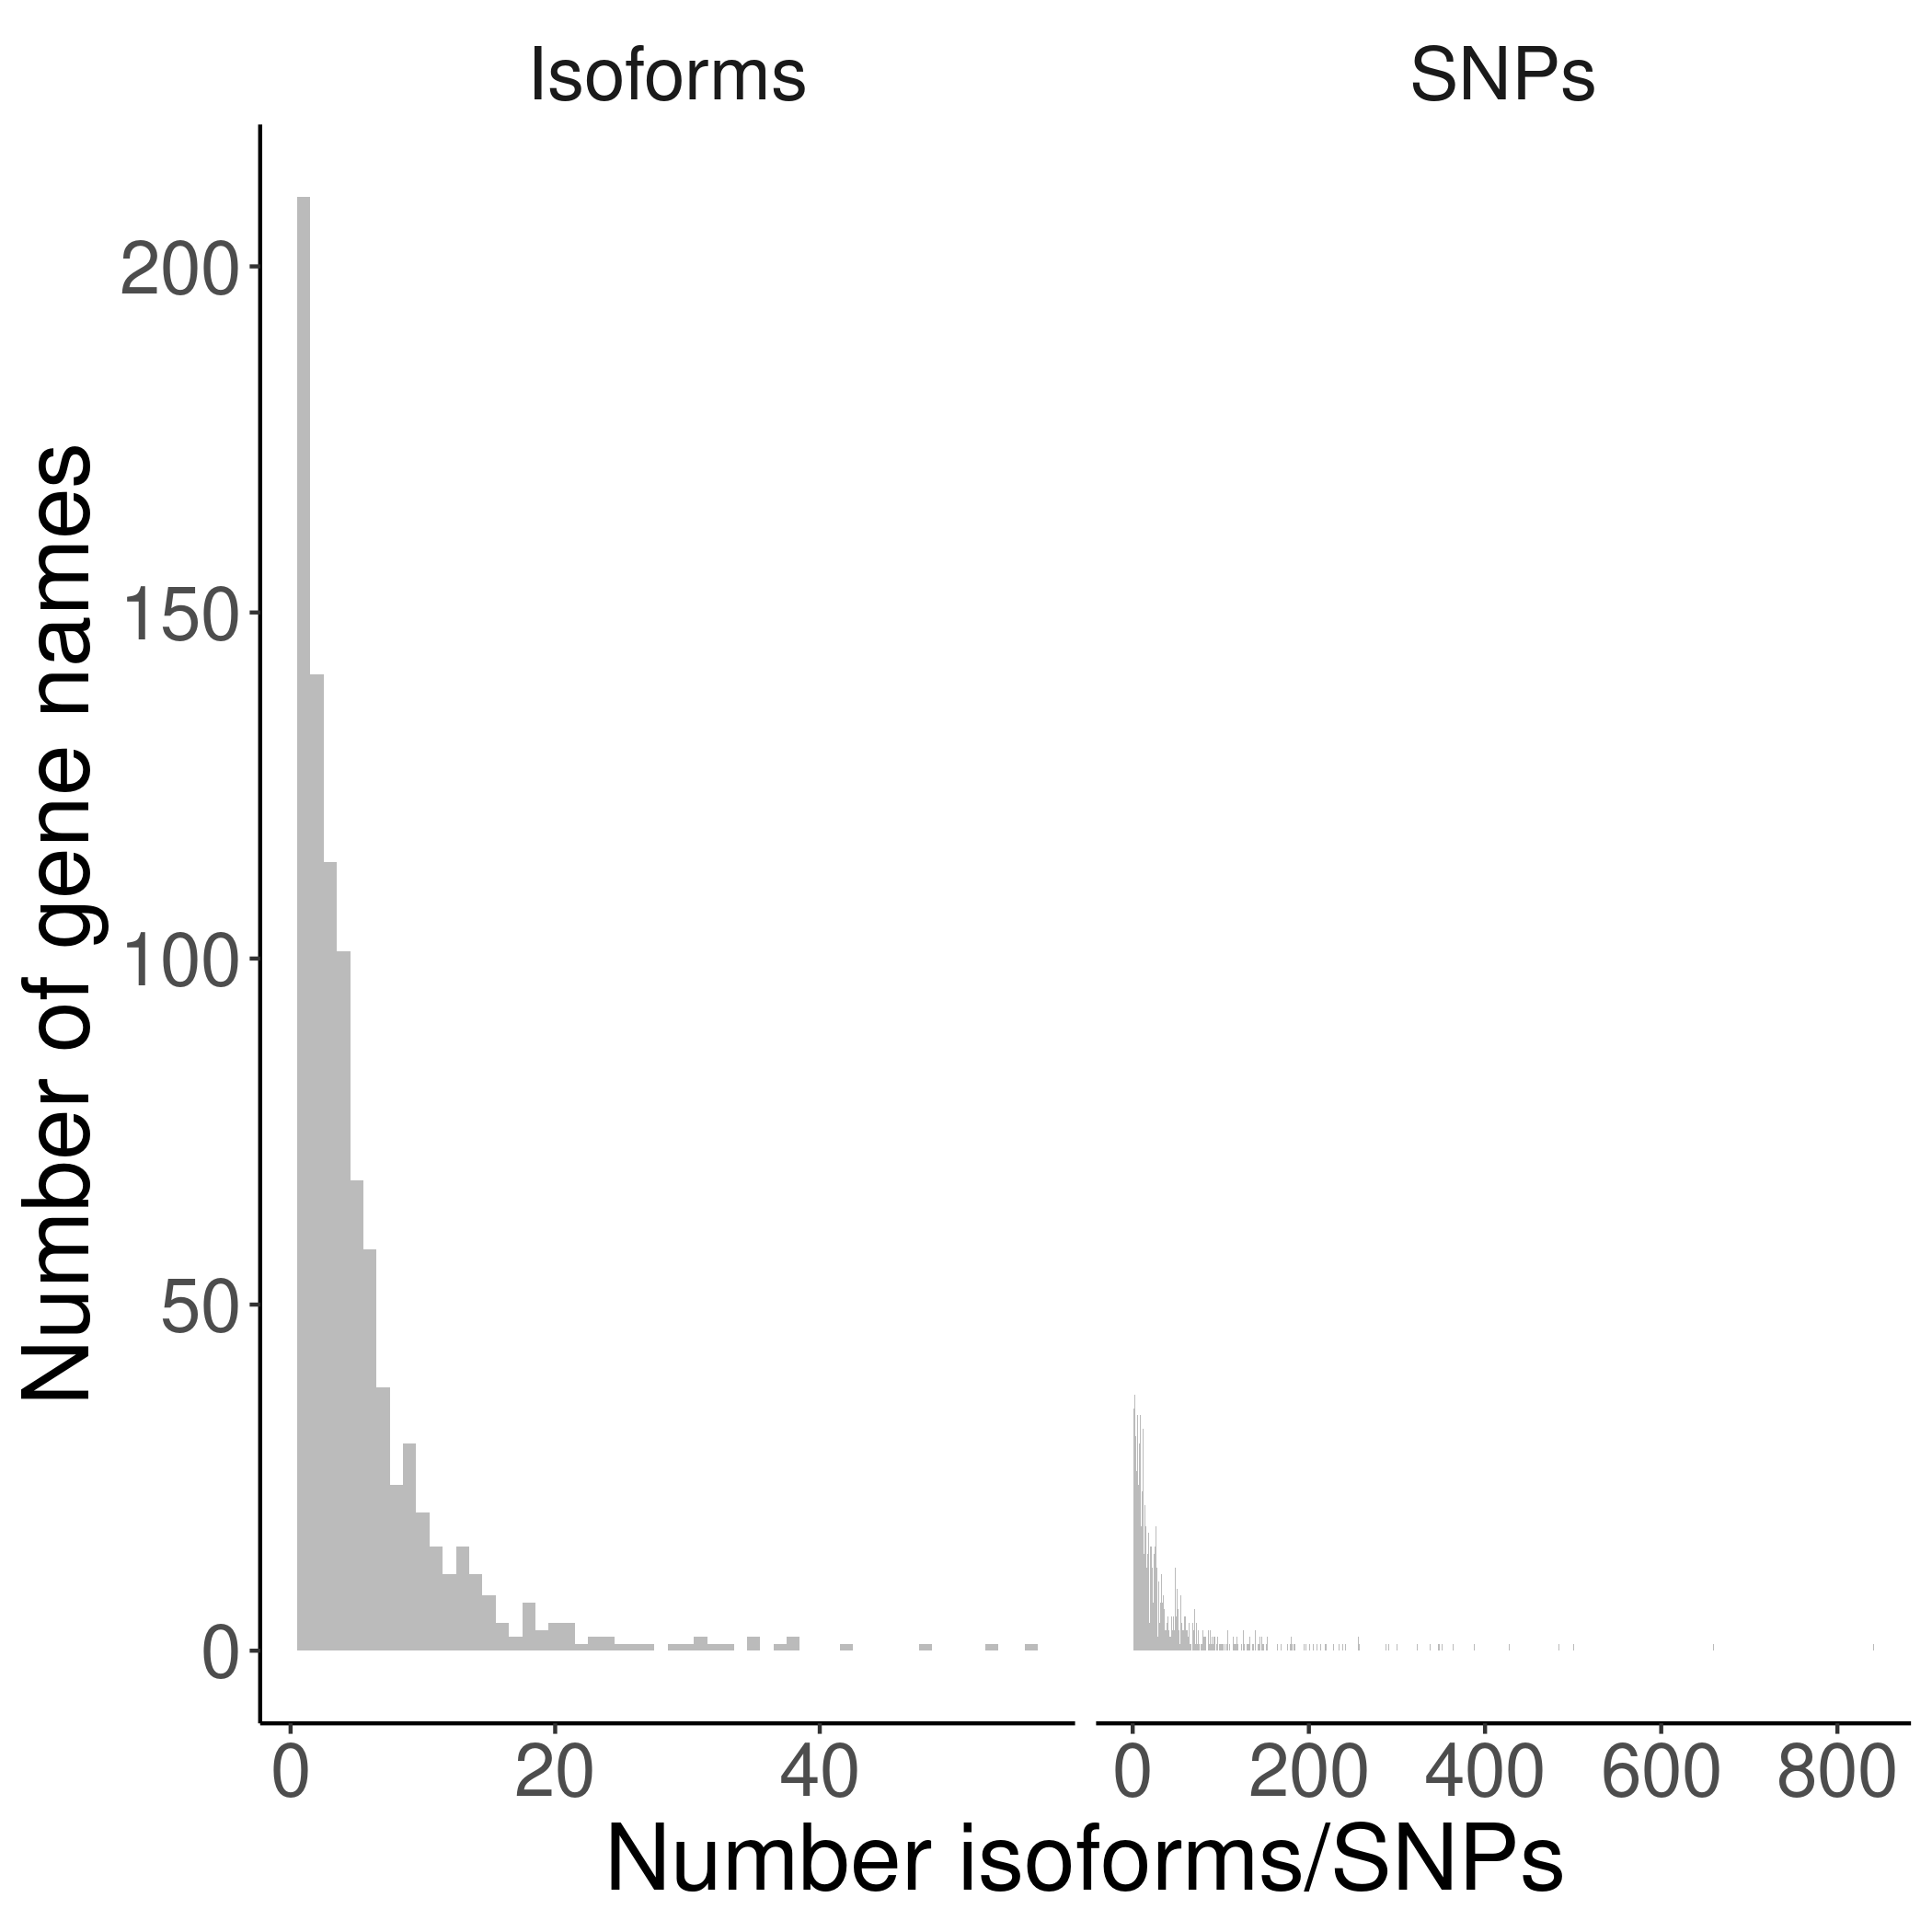
\includegraphics[width=\textwidth]{ncbi_peregrine_results/fig_n_proteins_per_gene_name.png}
  \caption{
    Histogram of the number of proteins found per gene name.
    Most often, a gene name is associated with one proteins. 
  }
  \label{fig:n_proteins_per_gene_name}
\end{figure}


\begin{figure}[!htbp]
  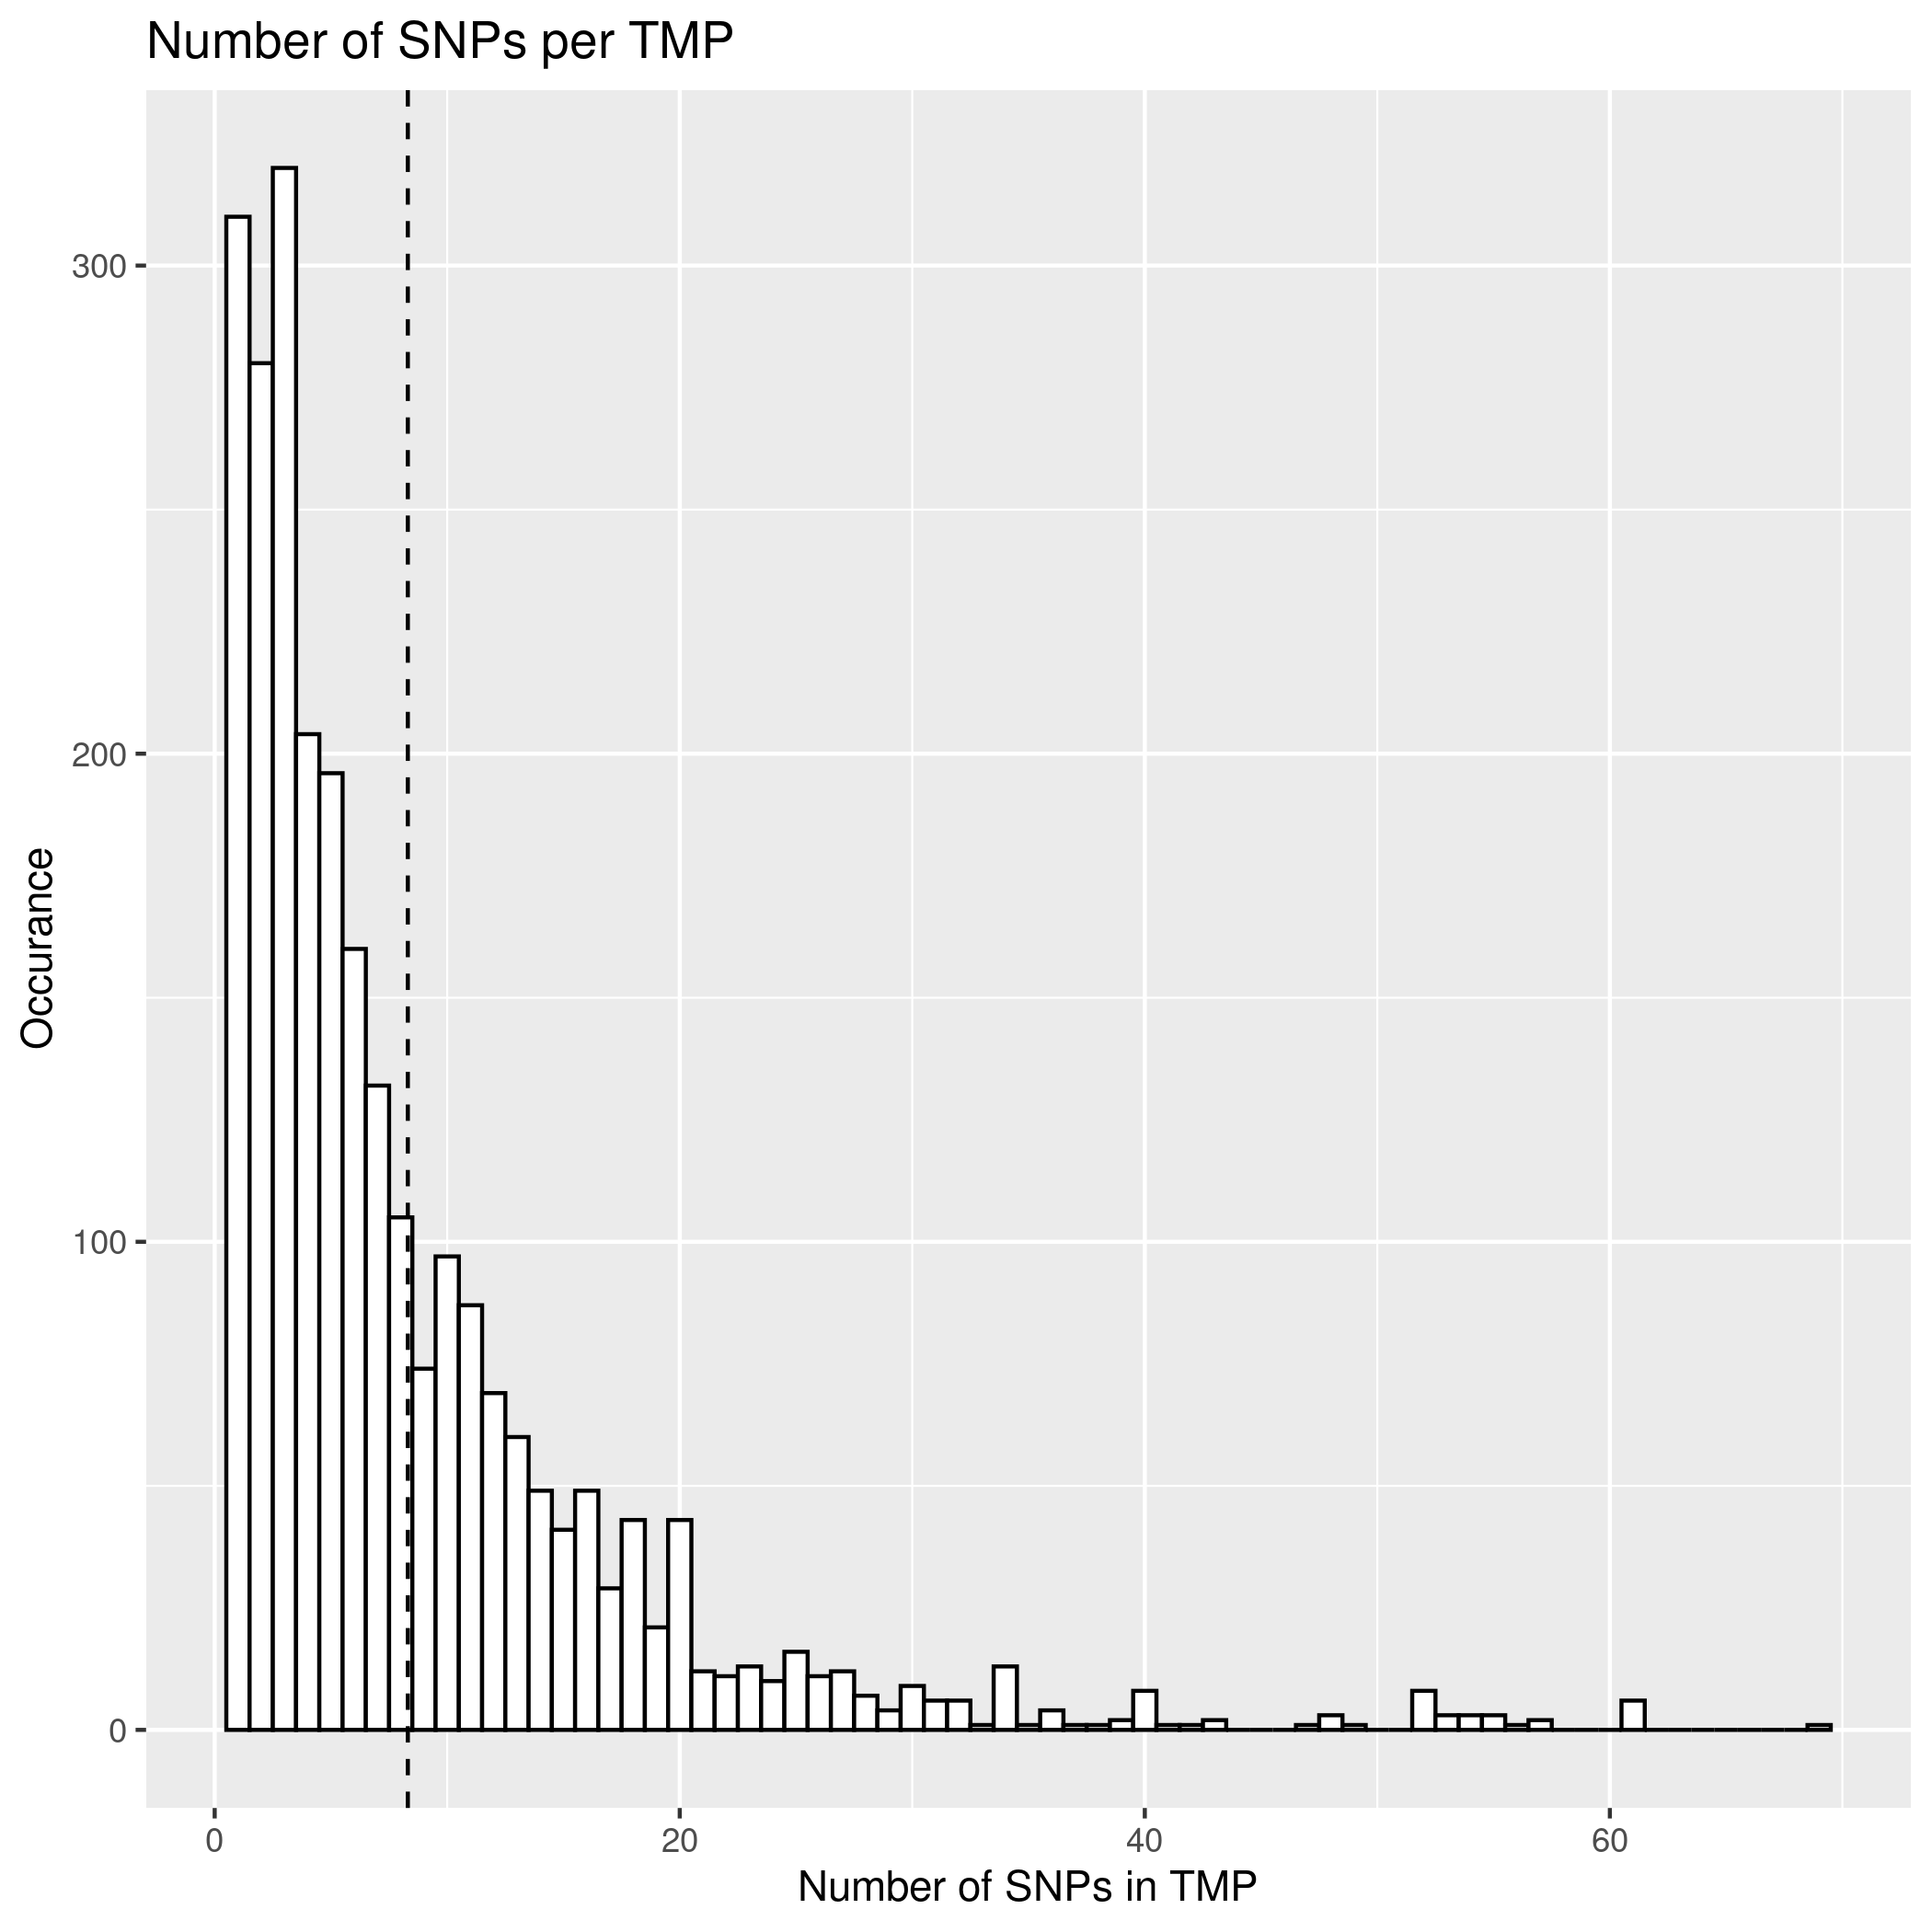
\includegraphics[width=\textwidth]{ncbi_peregrine_results/fig_n_snps_per_tmp.png}
  \caption{
    Histogram of the number of SNPs per trans-membrane protein.
    Dashed vertical line: average number of SNPs per TMP
  }
  \label{fig:fig_n_snps_per_tmp}
\end{figure}

\begin{figure}[!htbp]
  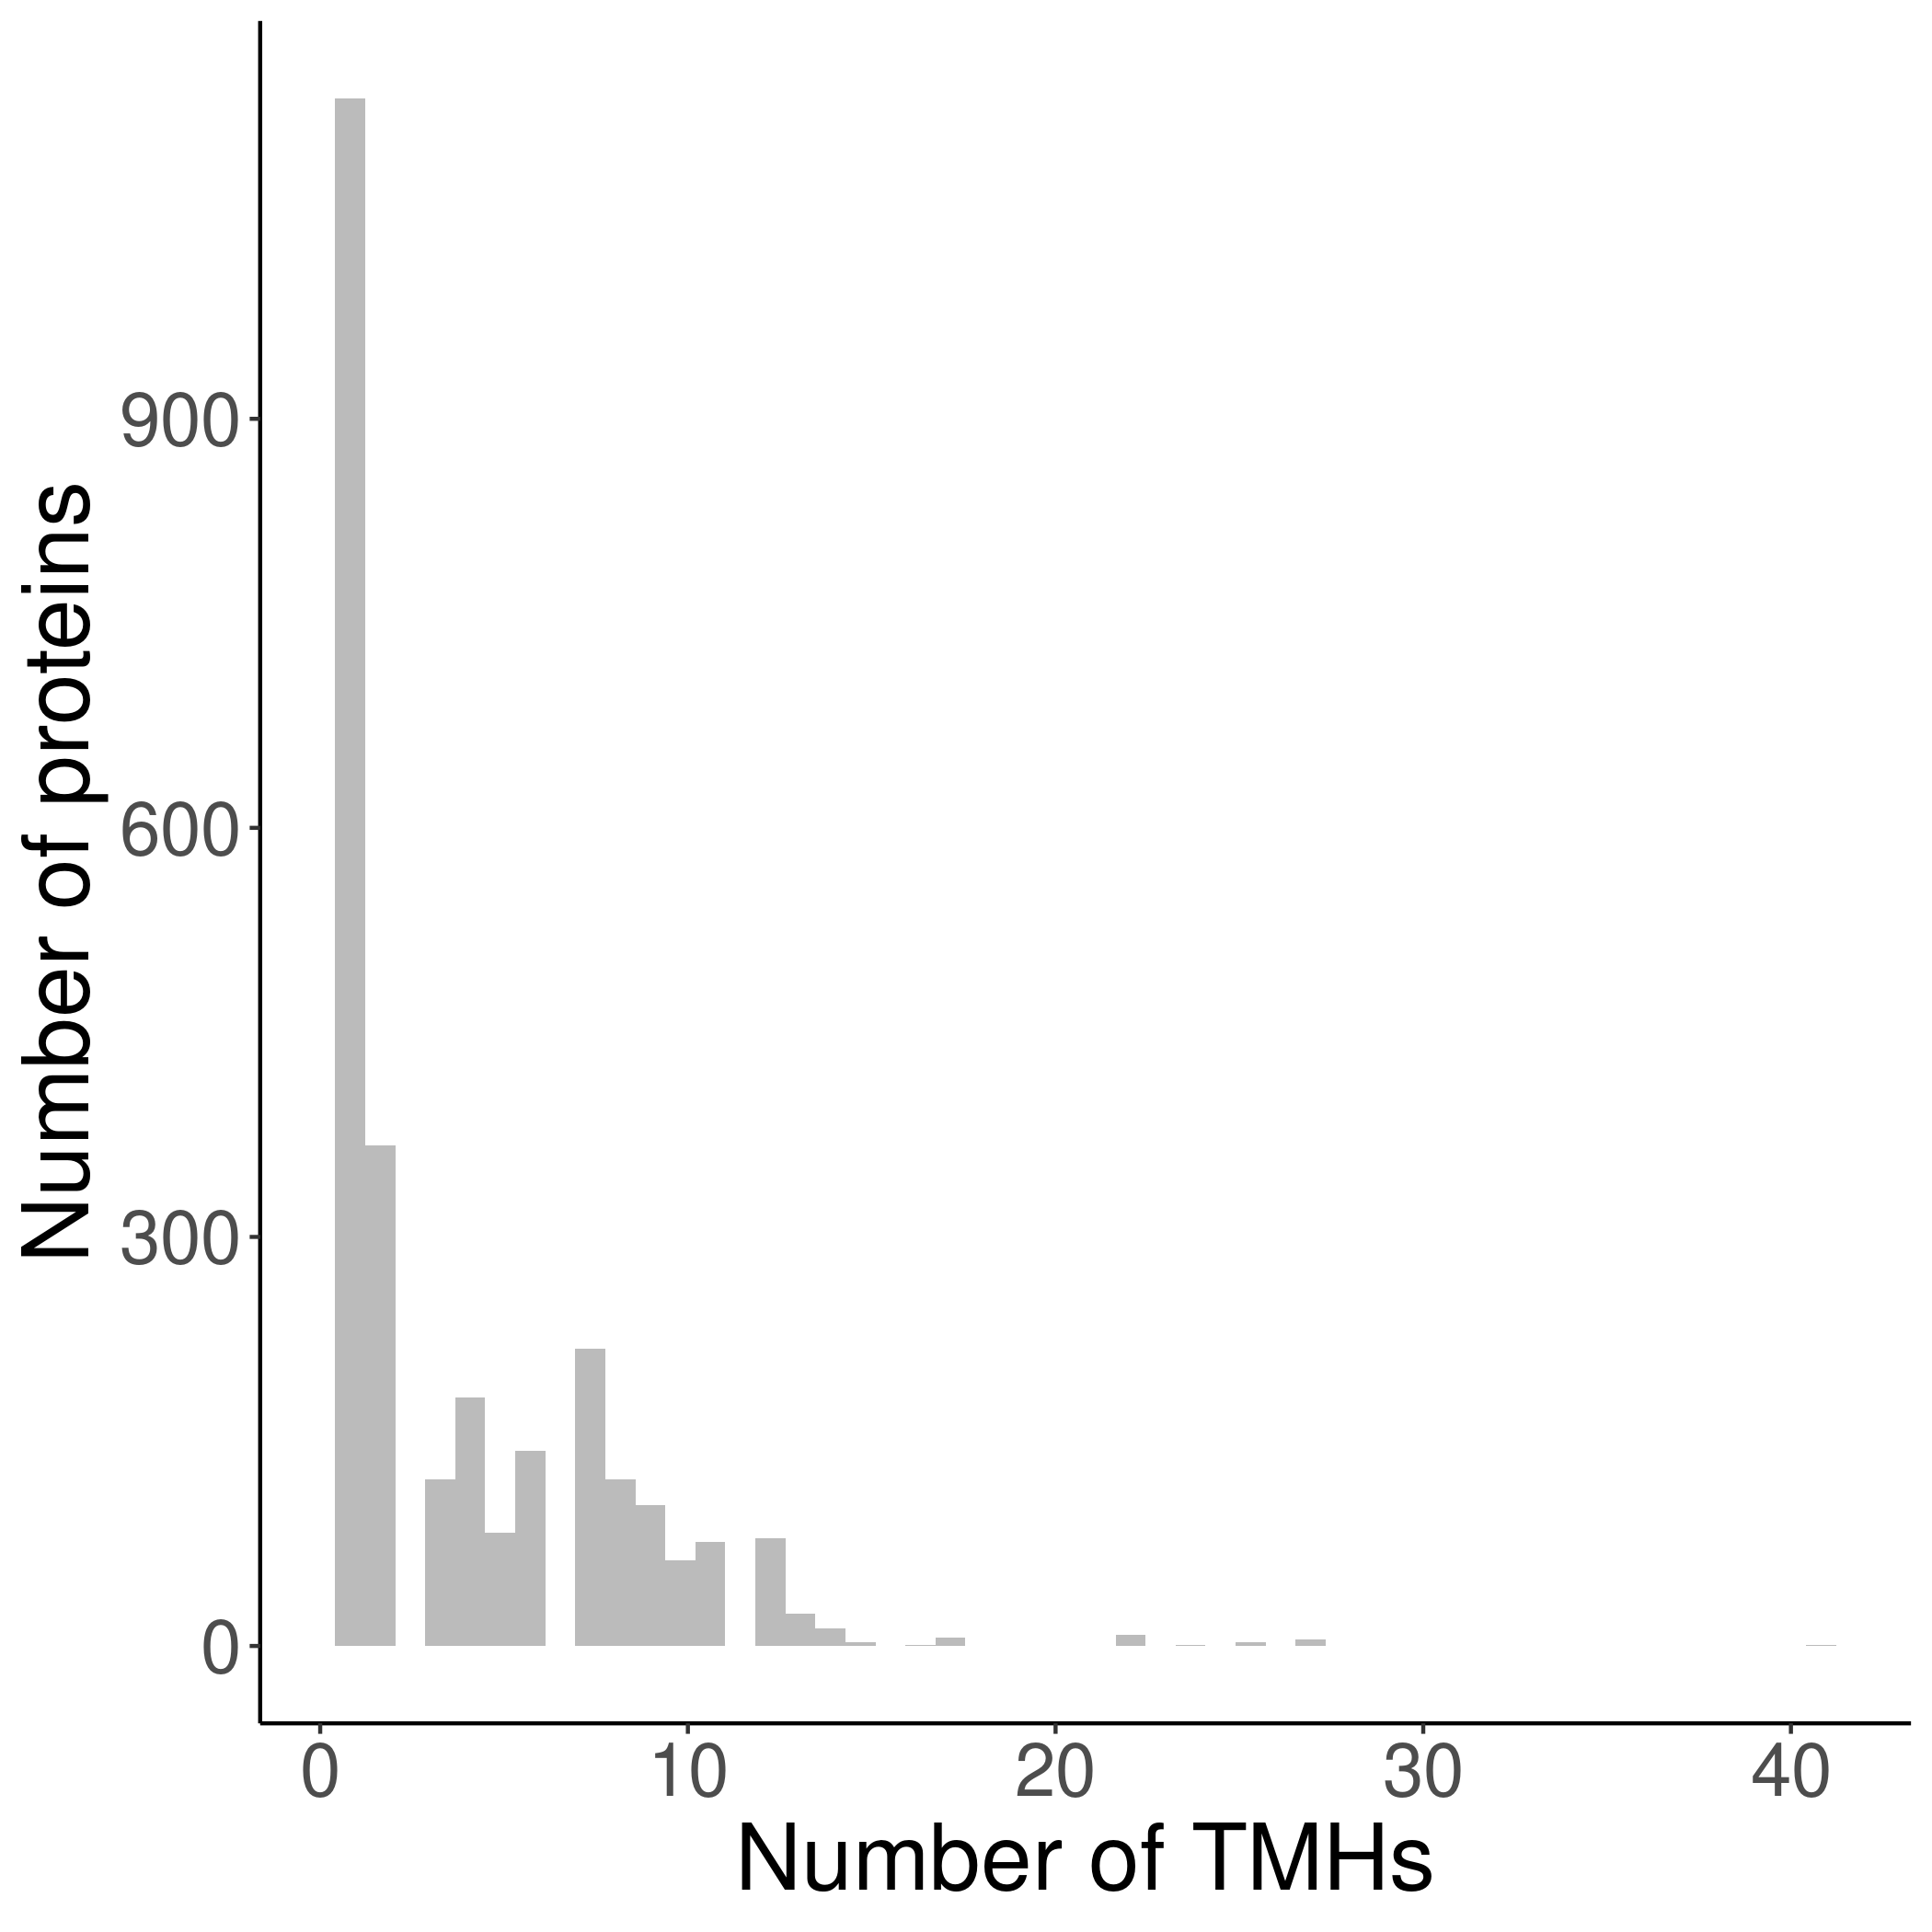
\includegraphics[width=\textwidth]{ncbi_peregrine_results/fig_n_tmhs_per_protein.png}
  \caption{
    Histogram of the number of TMHs predicted per protein,
    for the trans-membrane proteins used.
  }
  \label{fig:fig_n_tmhs_per_protein}
\end{figure}

\begin{figure}[!htbp]
  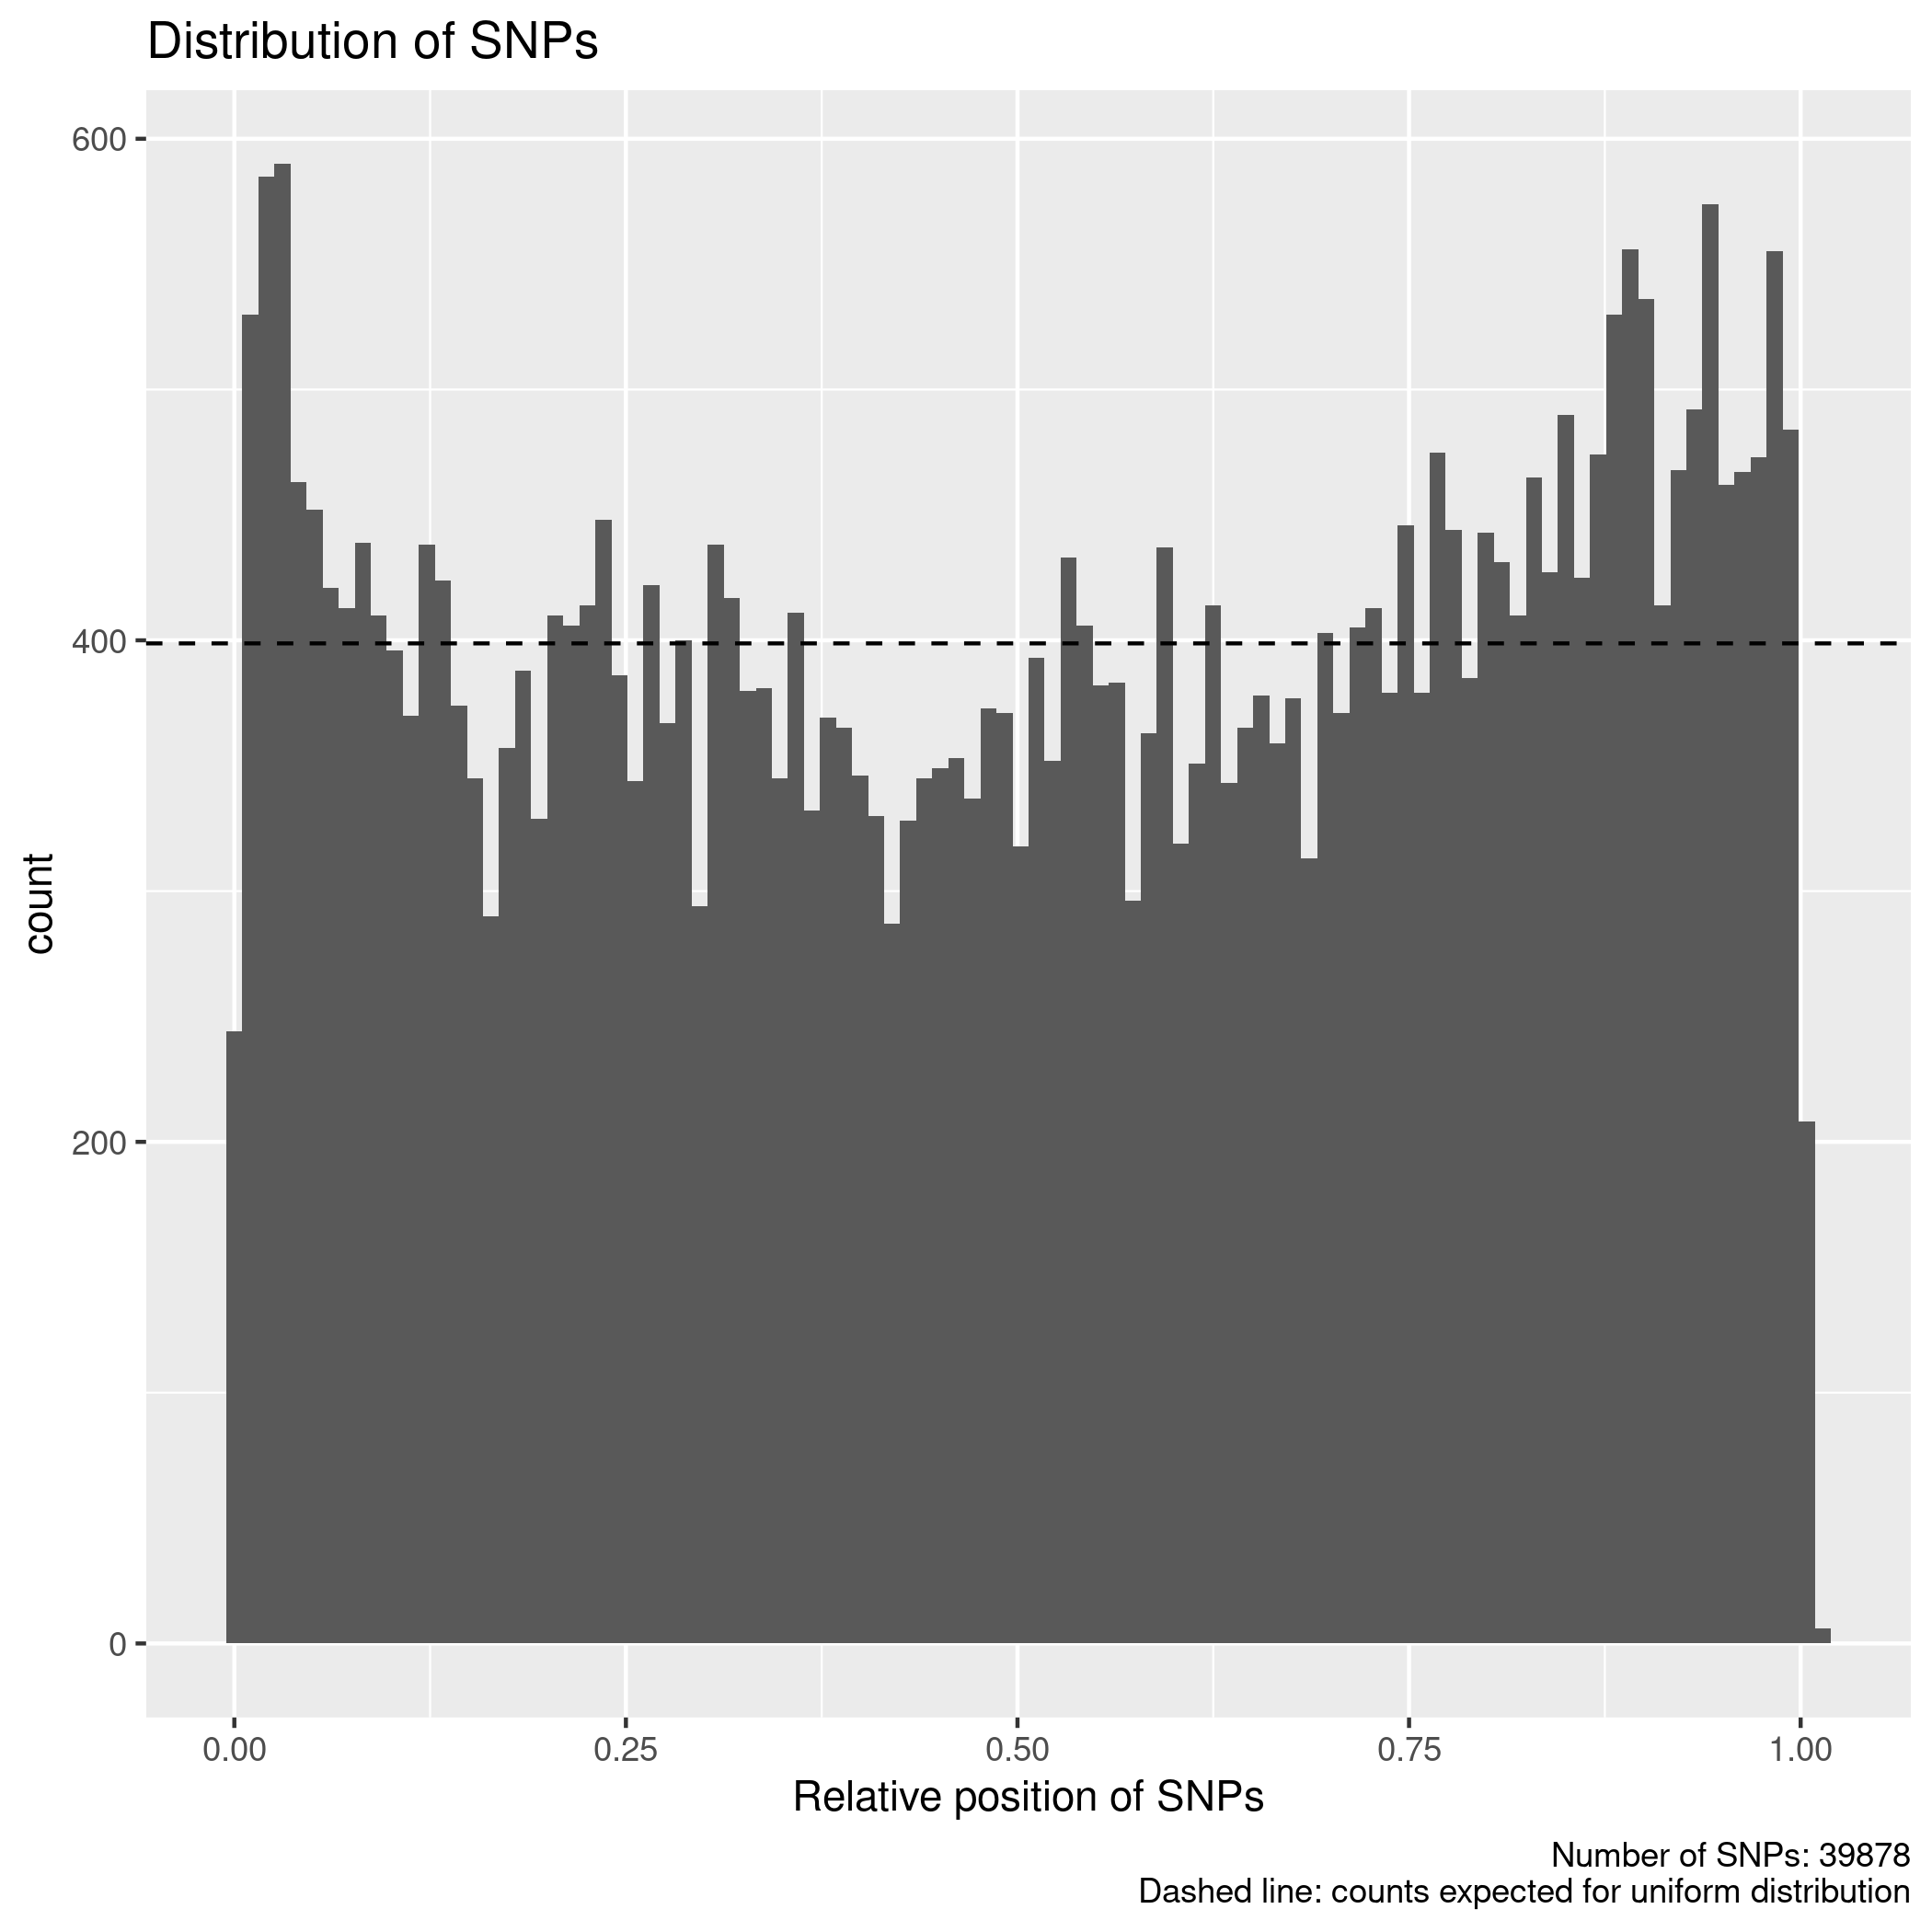
\includegraphics[width=\textwidth]{ncbi_peregrine_results/fig_snp_rel_pos.png}
  \caption{
    Distribution of the relative position of the SNPs used,
    where a relative position of zero denotes the first amino
    acid at the N-terminus, where a relative position of one
    indicates the last residue at the C-terminus.
  }
  \label{fig:snp_rel_pos}
\end{figure}

% \paragraph{Relative position of SNPs}

To verify if SNPs were sampled uniformly
over proteins, we show the distribution 
of the relative position in figure \ref{fig:snp_rel_pos}.
We find no clear evidence of a bias.

% \paragraph{Statistics}

Table \ref{tab:snp_stats} shows the statistics for all
SNPs, where tables \ref{tab:snp_stats_per_spanner_single}
and \ref{tab:snp_stats_per_spanner_multi} show the
statistics for only single-spanners and multi-spanners respectively.
 
% Label: tab:snp_stats
\begin{table}

\caption{\label{tab:snp_stats}Statistics for the multi-spanners. p = p value. n = number of SNPs. n\_success = number of SNPs found in TMHs (dashed blue line). E(n\_success) = expected number of SNPs to be found in TMHs (dashed red line). }
\centering
\begin{tabular}[t]{l|l}
\hline
parameter & value\\
\hline
p & 6.820823e-11\\
\hline
n & 21208\\
\hline
n\_success & 3803\\
\hline
E(n\_success) & 4140.56\\
\hline
\end{tabular}
\end{table}

% Label: tab:snp_stats_per_spanner_single
\begin{table}

\caption{\label{tab:snp_stats_per_spanner_single}Statistics for the single-spanners. p = p value. n = number of SNPs in single-spanners. n\_success = number of SNPs found in TMHs of single-spanners (dashed blue line). E(n\_success) = expected number of SNPs to be found in TMHs of single-spanners. }
\centering
\begin{tabular}[t]{l|l}
\hline
parameter & value\\
\hline
p & 0.3189532\\
\hline
n & 8186\\
\hline
n\_success & 452\\
\hline
E(n\_success) & 462.1535\\
\hline
\end{tabular}
\end{table}


% Label: tab:snp_stats_per_spanner_multi
\begin{table}

\caption{\label{tab:snp_stats_per_spanner_multi}Statistics for the multi-spanners. p = p value. n = number of SNPs in multi-spanners. n\_success = number of SNPs found in TMHs of multi-spanners (dashed blue line). E(n\_success) = expected number of SNPs to be found in TMHs of multi-spanners  (dashed red line). }
\centering
\begin{tabular}[t]{l|l}
\hline
parameter & value\\
\hline
p & 4.388709e-14\\
\hline
n & 13386\\
\hline
n\_success & 3377\\
\hline
E(n\_success) & 3767.26\\
\hline
\end{tabular}
\end{table}

%
% Notes to self
%

%\begin{sidewaystable}
%  \centering
%  ... centered table here
%\end{sidewaystable}

% \scalebox{0.7}{
%  ... scaled table here
% }

%{\tiny
%  ... something with a tiny font
%}

% Instead of non-TMH use 'soluble protein region'
% or 'cytosolic or extracellular protein region'

